\documentclass[12pt,]{article}
%\usepackage{lmodern}  Melissa removed to deal with font rendering issue
\usepackage{amssymb,amsmath}
\usepackage{ifxetex,ifluatex}
\usepackage{fixltx2e} % provides \textsubscript

%Melissa removed the following section to deal with font rendering issue
%\ifnum 0\ifxetex 1\fi\ifluatex 1\fi=0 % if pdftex
%  \usepackage[T1]{fontenc}
%  \usepackage[utf8]{inputenc}
%%\else % if luatex or xelatex
%  \ifxetex
%    \usepackage{mathspec}
%  \else
%    \usepackage{fontspec}
%  \fi
%  \defaultfontfeatures{Ligatures=TeX,Scale=MatchLowercase}
%  \newcommand{\euro}{€}
%%%%%%\fi

% use upquote if available, for straight quotes in verbatim environments
\IfFileExists{upquote.sty}{\usepackage{upquote}}{}
% use microtype if available
\IfFileExists{microtype.sty}{%
\usepackage{microtype}
\UseMicrotypeSet[protrusion]{basicmath} % disable protrusion for tt fonts
}{}
\usepackage[margin=1in]{geometry}
\usepackage{hyperref}
\PassOptionsToPackage{usenames,dvipsnames}{color} % color is loaded by hyperref
\hypersetup{unicode=true,
            pdftitle={Status of Pacific ocean perch (Sebastes alutus) along the US west coast in 2017},
            pdfborder={0 0 0},
            breaklinks=true}
\urlstyle{same}  % don't use monospace font for urls
\usepackage{graphicx,grffile}
\makeatletter
\def\maxwidth{\ifdim\Gin@nat@width>\linewidth\linewidth\else\Gin@nat@width\fi}
\def\maxheight{\ifdim\Gin@nat@height>\textheight\textheight\else\Gin@nat@height\fi}
\makeatother
% Scale images if necessary, so that they will not overflow the page
% margins by default, and it is still possible to overwrite the defaults
% using explicit options in \includegraphics[width, height, ...]{}
\setkeys{Gin}{width=\maxwidth,height=\maxheight,keepaspectratio}
\setlength{\parindent}{0pt}
\setlength{\parskip}{6pt plus 2pt minus 1pt}
\setlength{\emergencystretch}{3em}  % prevent overfull lines
\providecommand{\tightlist}{%
  \setlength{\itemsep}{0pt}\setlength{\parskip}{0pt}}
\setcounter{secnumdepth}{5}

%%% Use protect on footnotes to avoid problems with footnotes in titles
\let\rmarkdownfootnote\footnote%
\def\footnote{\protect\rmarkdownfootnote}

%%% Change title format to be more compact
\usepackage{titling}

% Create subtitle command for use in maketitle
\newcommand{\subtitle}[1]{
  \posttitle{
    \begin{center}\large#1\end{center}
    }
}

\setlength{\droptitle}{-2em}
  \title{Status of Pacific ocean perch (\emph{Sebastes alutus}) along the US west
coast in 2017}
  \pretitle{\vspace{\droptitle}\centering\huge}
  \posttitle{\par}
  \author{}
  \preauthor{}\postauthor{}
  \date{}
  \predate{}\postdate{}


% This file contains all of the LaTeX packages you may need to compile the document
% Documentation for each package can be found onlines
\usepackage{tabularx}                                             % table environment providing flexibility
\usepackage{caption}                                              % for creating captions  
\usepackage{longtable}                                            % allows tables to span multiple pages
\usepackage{tabu}
\usepackage{rotating}                                             % allows for sideways tables
%\usepackage{float}                                                % floating environments; may not need in rmarkdown
\usepackage{placeins}                                             % keeps floats from moving
\usepackage{floatrow}                                             % package to put table captions at the top
\floatsetup[table]{capposition = top}                             % line to put captions at the top of pander tables
\usepackage{indentfirst}                                          % indents first paragraph of a section
\usepackage{mdwtab}                                               % continued float multi-page figure
\usepackage{enumerate}                                            % create lists
\usepackage{hyperref}                                             % highlight cross references
\hypersetup{colorlinks=true, urlcolor=blue, linktoc=page, linkcolor=blue, citecolor=blue} %define referencing colors
%\usepackage{makebox}                                             % make boxes around text
\usepackage[usenames,dvipsnames]{xcolor}                          % color name options
%\usepackage[space]{grffile}                                      % spaces in file name path
\usepackage{soul}                                                 % highlight text
\usepackage{enumitem}                                             % numbered lists
\usepackage{lineno}                                               % Line numbers; comment out for final
\usepackage{upquote}                                              % produce grave accent in latex
\usepackage{verbatim}                                             % produces verbatim results
\usepackage{fancyvrb}                                             % verbatim in a box
%\usepackage{draftwatermark}                                      % places Draft watermark in background; comment out for final
\usepackage{textcomp}                                             % fixes error with packages interfering
\usepackage{lscape}                                               % rotate pages - to allow for landscape longtables
%\pdfinterwordspaceon                                             % fix loss of inter word spacing
\usepackage{cmap}                                                 % fix mapping characters to unicode
\RequirePackage[linewidth = 1]{pdfcomment}                        % pdf comments
\RequirePackage[l2tabu, orthodox]{nag}                            % checks packages related to the accessibility?
\usepackage[inline]{showlabels}                                   % show table and figure labels; comment out for final
%\RequirePackage[tagged]{accessibilityMeta}


\linenumbers                                                      % specify use of line numbers


\definecolor{light-gray}{gray}{.85}                               % define light-gray as a color
%\usepackage[tagged]{accessibility-meta}

 
%\showlabels[\color{mred}]{label}

% Redefines (sub)paragraphs to behave more like sections
\ifx\paragraph\undefined\else
\let\oldparagraph\paragraph
\renewcommand{\paragraph}[1]{\oldparagraph{#1}\mbox{}}
\fi
\ifx\subparagraph\undefined\else
\let\oldsubparagraph\subparagraph
\renewcommand{\subparagraph}[1]{\oldsubparagraph{#1}\mbox{}}
\fi

\begin{document}
\maketitle


\begin{center}
\thispagestyle{empty}


\vspace{.5cm}

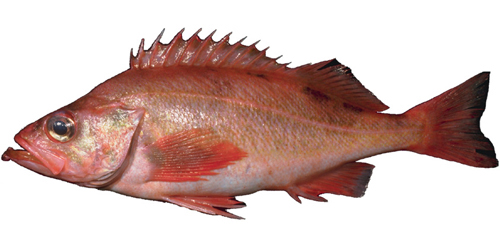
\includegraphics{Sebastes_alutus}~\\[0.5cm]
%\pdftooltip{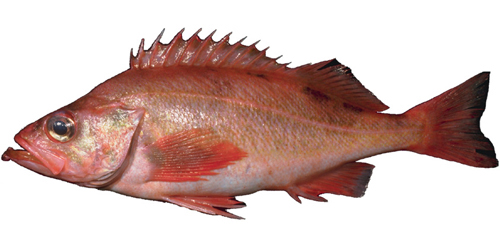
\includegraphics{Sebastes_alutus}}{This is a fish.}



Chantel R. Wetzel\textsuperscript{1}\\
Kelli Johnson\textsuperscript{1}\\
Lee Cronin-Fine\textsuperscript{2}\\

\vspace{.5cm}

\small
\textsuperscript{1}Northwest Fisheries Science Center, U.S. Department of Commerce, National Oceanic and Atmospheric Administration, National Marine Fisheries Service, 2725 Montlake Boulevard East, Seattle, Washington 98112\\

\vspace{.3cm}

\textsuperscript{3}University of Washington, School of Aquatic and Fishery Sciences\\

\vspace{.3cm}

%\textsuperscript{4}Oregon Department of Fish and Wildlife, 2040 SE Marine Science Drive, Newport, OR 97365\\


\vspace{.5cm}

\vfill
DRAFT SAFE\\
Disclaimer: This information is distributed solely for the purpose of pre-dissemination
peer review under applicable information quality guidelines. It has not been formally
disseminated by NOAA Fisheries. It does not represent and should not be construed to
represent any agency determination or policy. 

\vspace{.3cm}
%Bottom of the page
%{\large \today}

\maketitle

\pagenumbering{roman}
\setcounter{page}{1}
\end{center}

{
\setcounter{tocdepth}{4}
\tableofcontents
}
\setlength{\parskip}{5mm plus1mm minus1mm} \pagebreak

\pagenumbering{arabic} \setcounter{page}{1}
\renewcommand{\thefigure}{\alph{figure}}
\renewcommand{\thetable}{\alph{table}}

\section*{Executive Summary}\label{executive-summary}
\addcontentsline{toc}{section}{Executive Summary}

\subsection*{Stock}\label{stock}
\addcontentsline{toc}{subsection}{Stock}

This assessment reports the status of the Pacific ocean perch
(\emph{Sebastes alutus}) speciess off rockfish off the U.S. West Coast
from Northern California to the Canadian Border using data through 2017.
Pacific ocean perch are most abundant in the Gulf of Alaska and have
observed off of Japan, in the Bering Sea, and south to Baja California,
although they are sparse south of Oregon and rare in southern
California. \hl{Composition data indicate that
good recruitment years coincide in Oregon and Washington.} To date, no
significant genetic differences have been found in the range covered by
this assessment.

\subsection*{Landings}\label{landings}
\addcontentsline{toc}{subsection}{Landings}

The first year that harvest of Pacific ocean perch exceeded 1 mt off the
U.S. West Coast first occured in 1929. Catches ramped up in the 1940s
with large removals in Washington waters. During the 1950s the removals
primarly occured in Oregon waters with catches from Washington declining
following the 1940s. The largest removals in 1966-1968 were largely a
result of harvest by foreing vessels. The fishery proceed with more
moderate removals ranging between 1,200 to 2,600 metric tons per year
between 1969 to 1980. Removals generally decined from 1981 to 1994 to
between 1,000 and 1,700 metric tons per year. Pacific ocean perch was
declared overfished in 1999 resulting in large reduction in harvest in
recent years since the declaration.

\begin{table}[ht]
\centering
\caption{Landings (mt) for the past 10 years for Pacific ocean perch by fleet.} 
\label{tab:Exec_catch}
\begin{tabular}{l>{\centering}p{0.7in}>{\centering}p{0.7in}>{\centering}p{0.7in}>{\centering}p{0.7in}>{\centering}p{0.7in}>{\centering}p{0.7in}}
  \hline
Year & California & Oregon & Washington & At-sea Hake & Research & Total Landings \\ 
  \hline
2007 & 0.15 & 83.65 & 45.12 & 4.05 & 0.58 & 133.55 \\ 
  2008 & 0.39 & 58.64 & 16.61 & 15.93 & 0.80 & 92.37 \\ 
  2009 & 0.92 & 58.75 & 33.22 & 1.56 & 2.72 & 97.17 \\ 
  2010 & 0.14 & 58.00 & 22.29 & 16.87 & 1.68 & 98.98 \\ 
  2011 & 0.12 & 30.26 & 19.66 & 9.17 & 1.94 & 61.14 \\ 
  2012 & 0.18 & 30.41 & 21.79 & 4.52 & 1.62 & 58.51 \\ 
  2013 & 0.08 & 34.86 & 14.83 & 5.41 & 1.71 & 56.89 \\ 
  2014 & 0.18 & 33.92 & 15.82 & 3.92 & 0.57 & 54.41 \\ 
  2015 & 0.12 & 38.12 & 11.41 & 8.71 & 1.59 & 59.95 \\ 
  2016 & 0.19 & 34.15 & 13.12 & 10.30 & 0.12 & 57.87 \\ 
   \hline
\end{tabular}
\end{table}

\FloatBarrier

\begin{figure}
\centering
\includegraphics{PacificOceanPerch2017_Assessment_files/figure-latex/unnamed-chunk-11-1.pdf}
\caption{Landings of Pacific ocean perch for California, Oregon,
Washington, the Foriegn fishery (1966-1976), At-Sea Hake fishery, and
fishery independent surveys. \label{fig:Exec_catch1}}
\end{figure}

\subsection*{Data and Assessment}\label{data-and-assessment}
\addcontentsline{toc}{subsection}{Data and Assessment}

This a new full assessment for Pacific ocean perch which was last
assessed in 2011. In this assessment, all aspects of the model including
catches, data, and modelling assumptions were re-evaluated as much as
possible. The assessment was conducted using the length- and
age-structured modeling software Stock Synthesis (version 3.30). The
coastwide population was modeled assuming separate growth and mortality
parameters for each sex (a two-sex model) from 1918 to 2017, and
forecasted beyond 2017.

\FloatBarrier

\subsection*{Stock Biomass}\label{stock-biomass}
\addcontentsline{toc}{subsection}{Stock Biomass}

\hl{Include: trends and current levels relative to virgin or historic levels, 
description of uncertainty-include table for last 10 years and graph with 
long term estimates.}

Spawning output Figure: Figure \ref{fig:Spawnbio_all}\\
Spawning output Table(s): Table \ref{tab:SpawningDeplete_mod1}\\
Relative depletion Figure: Figure \ref{fig:RelDeplete_all}

Example text (remove Models 2 and 3 if not needed - if using, remove the
\# in-line comments!!!)\\
The estimated relative depletion level (spawning output relative to
unfished spawning output) of the the base-case model in 2017 is 38\%
(\textasciitilde{}95\% asymptotic interval: \(\pm\) -18.2\%-94.1\%)
(Figure \ref{fig:RelDeplete_all}).

\FloatBarrier

\begin{table}[ht]
\centering
\caption{Recent trend in estimated spawning output (million eggs) and relative spawning output.} 
\label{tab:SpawningDeplete_mod1}
\begin{tabular}{l>{\centering}p{1.3in}>{\centering}p{1.2in}>{\centering}p{1in}>{\centering}p{1.2in}}
  \hline
Year & Spawning Output (million eggs) & \~{} 95\% confidence interval & Estimated depletion & \~{} 95\% confidence interval \\ 
  \hline
2008 & 1100.00 & -590 - 2790 & 0.19 & -0.084 - 0.472 \\ 
  2009 & 1155.00 & -628 - 2939 & 0.20 & -0.090 - 0.498 \\ 
  2010 & 1203.00 & -664 - 3070 & 0.21 & -0.095 - 0.520 \\ 
  2011 & 1245.00 & -698 - 3189 & 0.22 & -0.101 - 0.540 \\ 
  2012 & 1288.00 & -726 - 3302 & 0.23 & -0.105 - 0.560 \\ 
  2013 & 1336.00 & -757 - 3429 & 0.24 & -0.110 - 0.581 \\ 
  2014 & 1442.00 & -820 - 3704 & 0.26 & -0.119 - 0.628 \\ 
  2015 & 1656.00 & -946 - 4258 & 0.29 & -0.137 - 0.722 \\ 
  2016 & 1919.00 & -1104 - 4942 & 0.34 & -0.161 - 0.838 \\ 
  2017 & 2151.00 & -1245 - 5547 & 0.38 & -0.182 - 0.941 \\ 
   \hline
\end{tabular}
\end{table}

\FloatBarrier

\begin{figure}
\centering
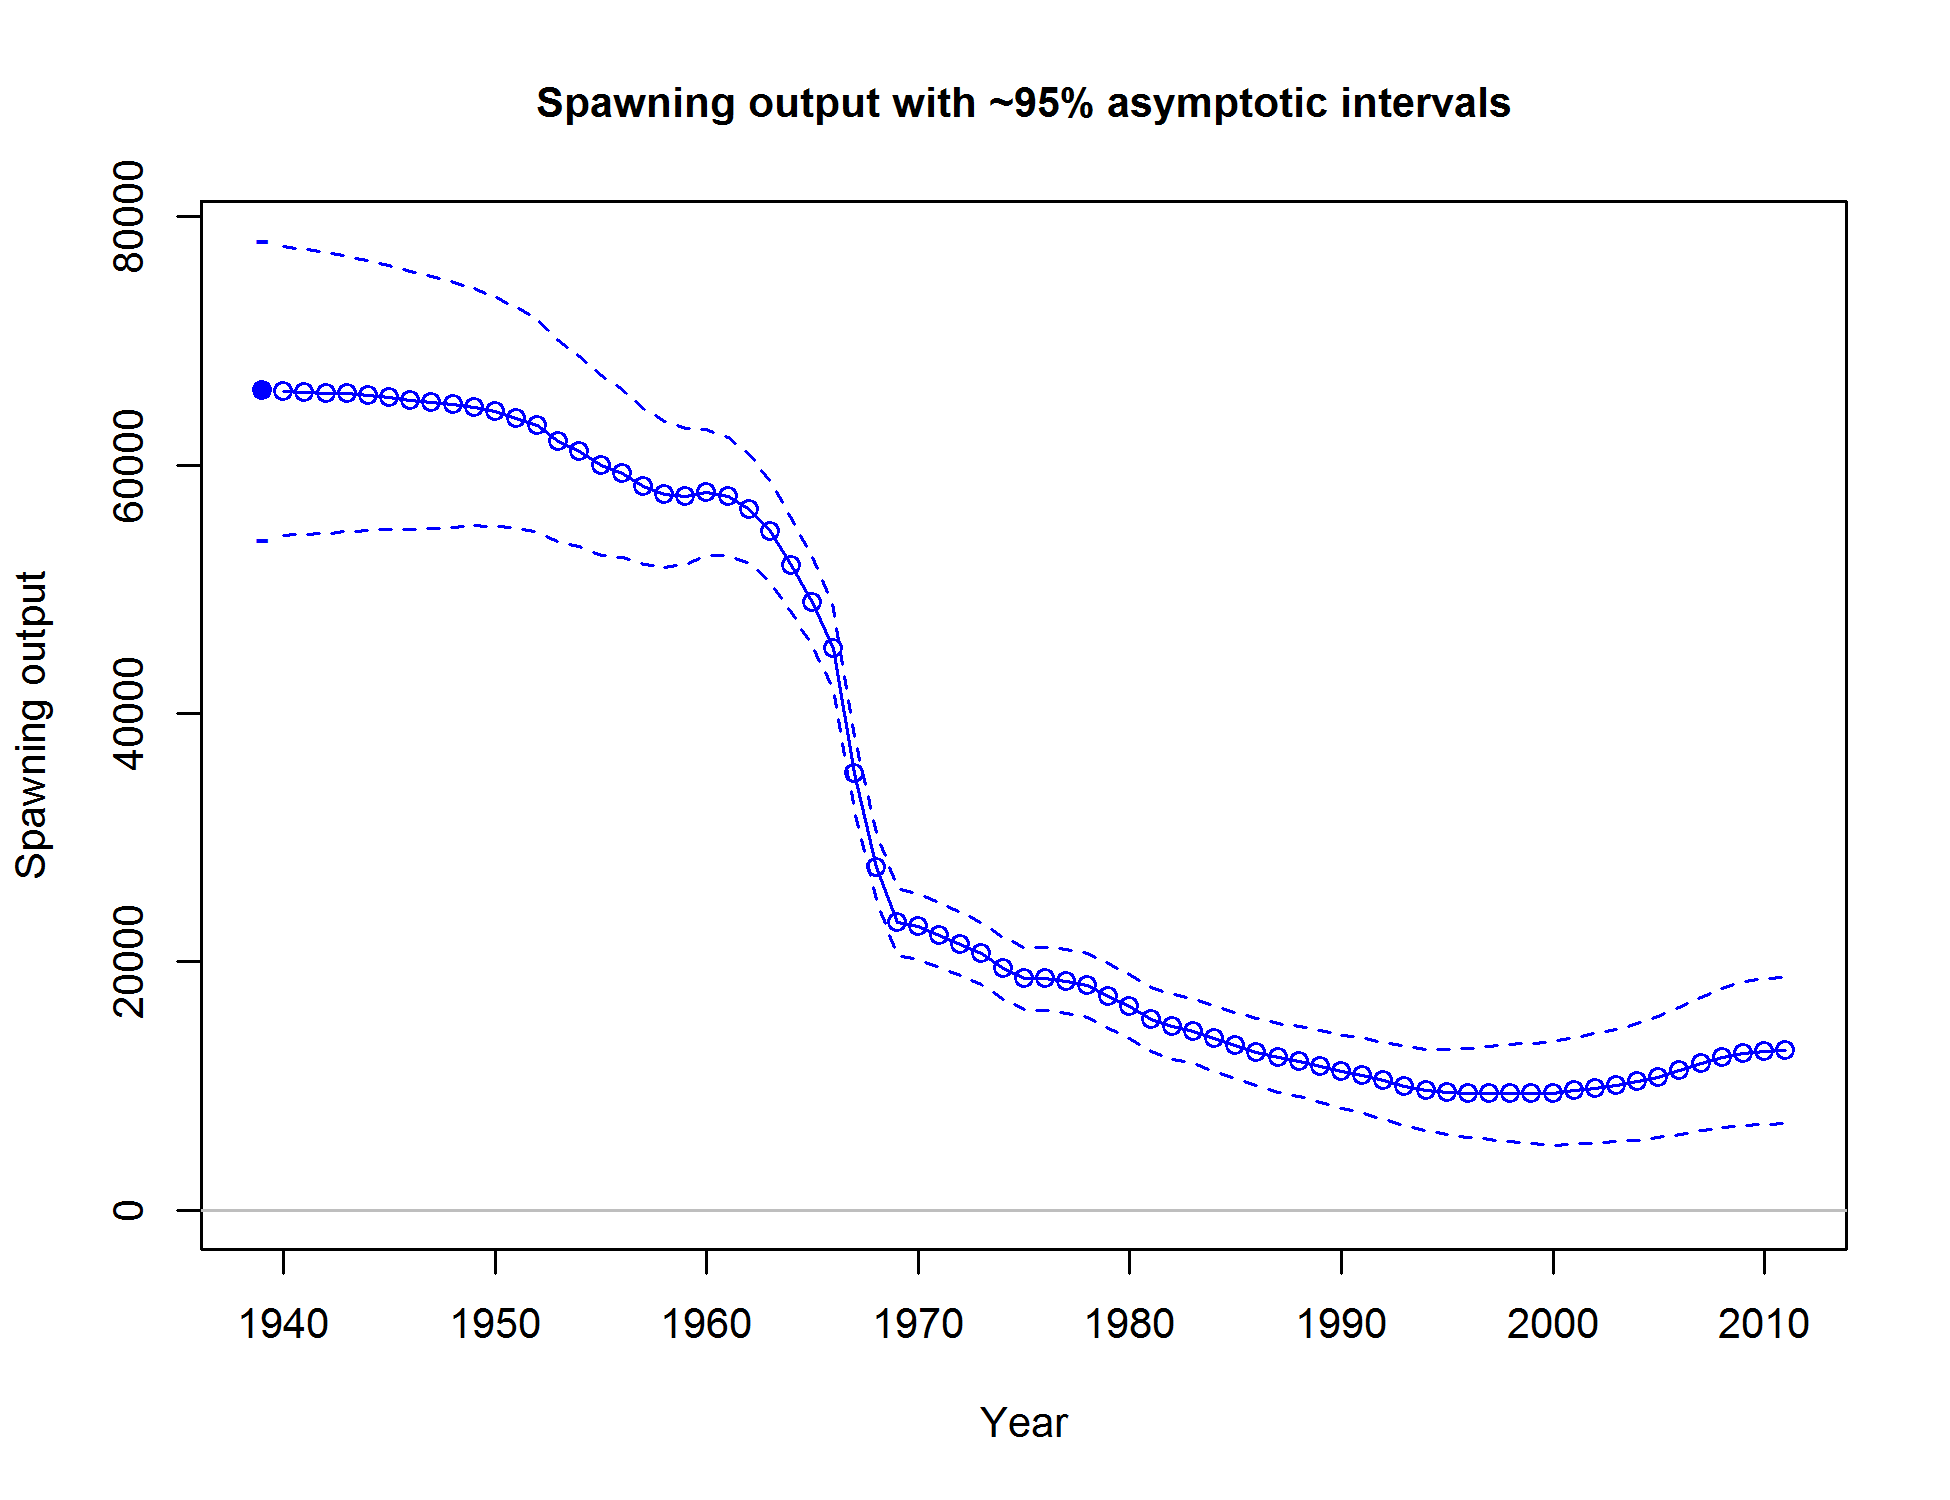
\includegraphics{r4ss/plots_mod1/ts7_Spawning_output_with_95_asymptotic_intervals_intervals.png}
\caption{Time series of spawning output trajectory (circles and line:
median; light broken lines: 95\% credibility intervals) for the base
case assessment model. \label{fig:Spawnbio_all}}
\end{figure}

\begin{figure}
\centering
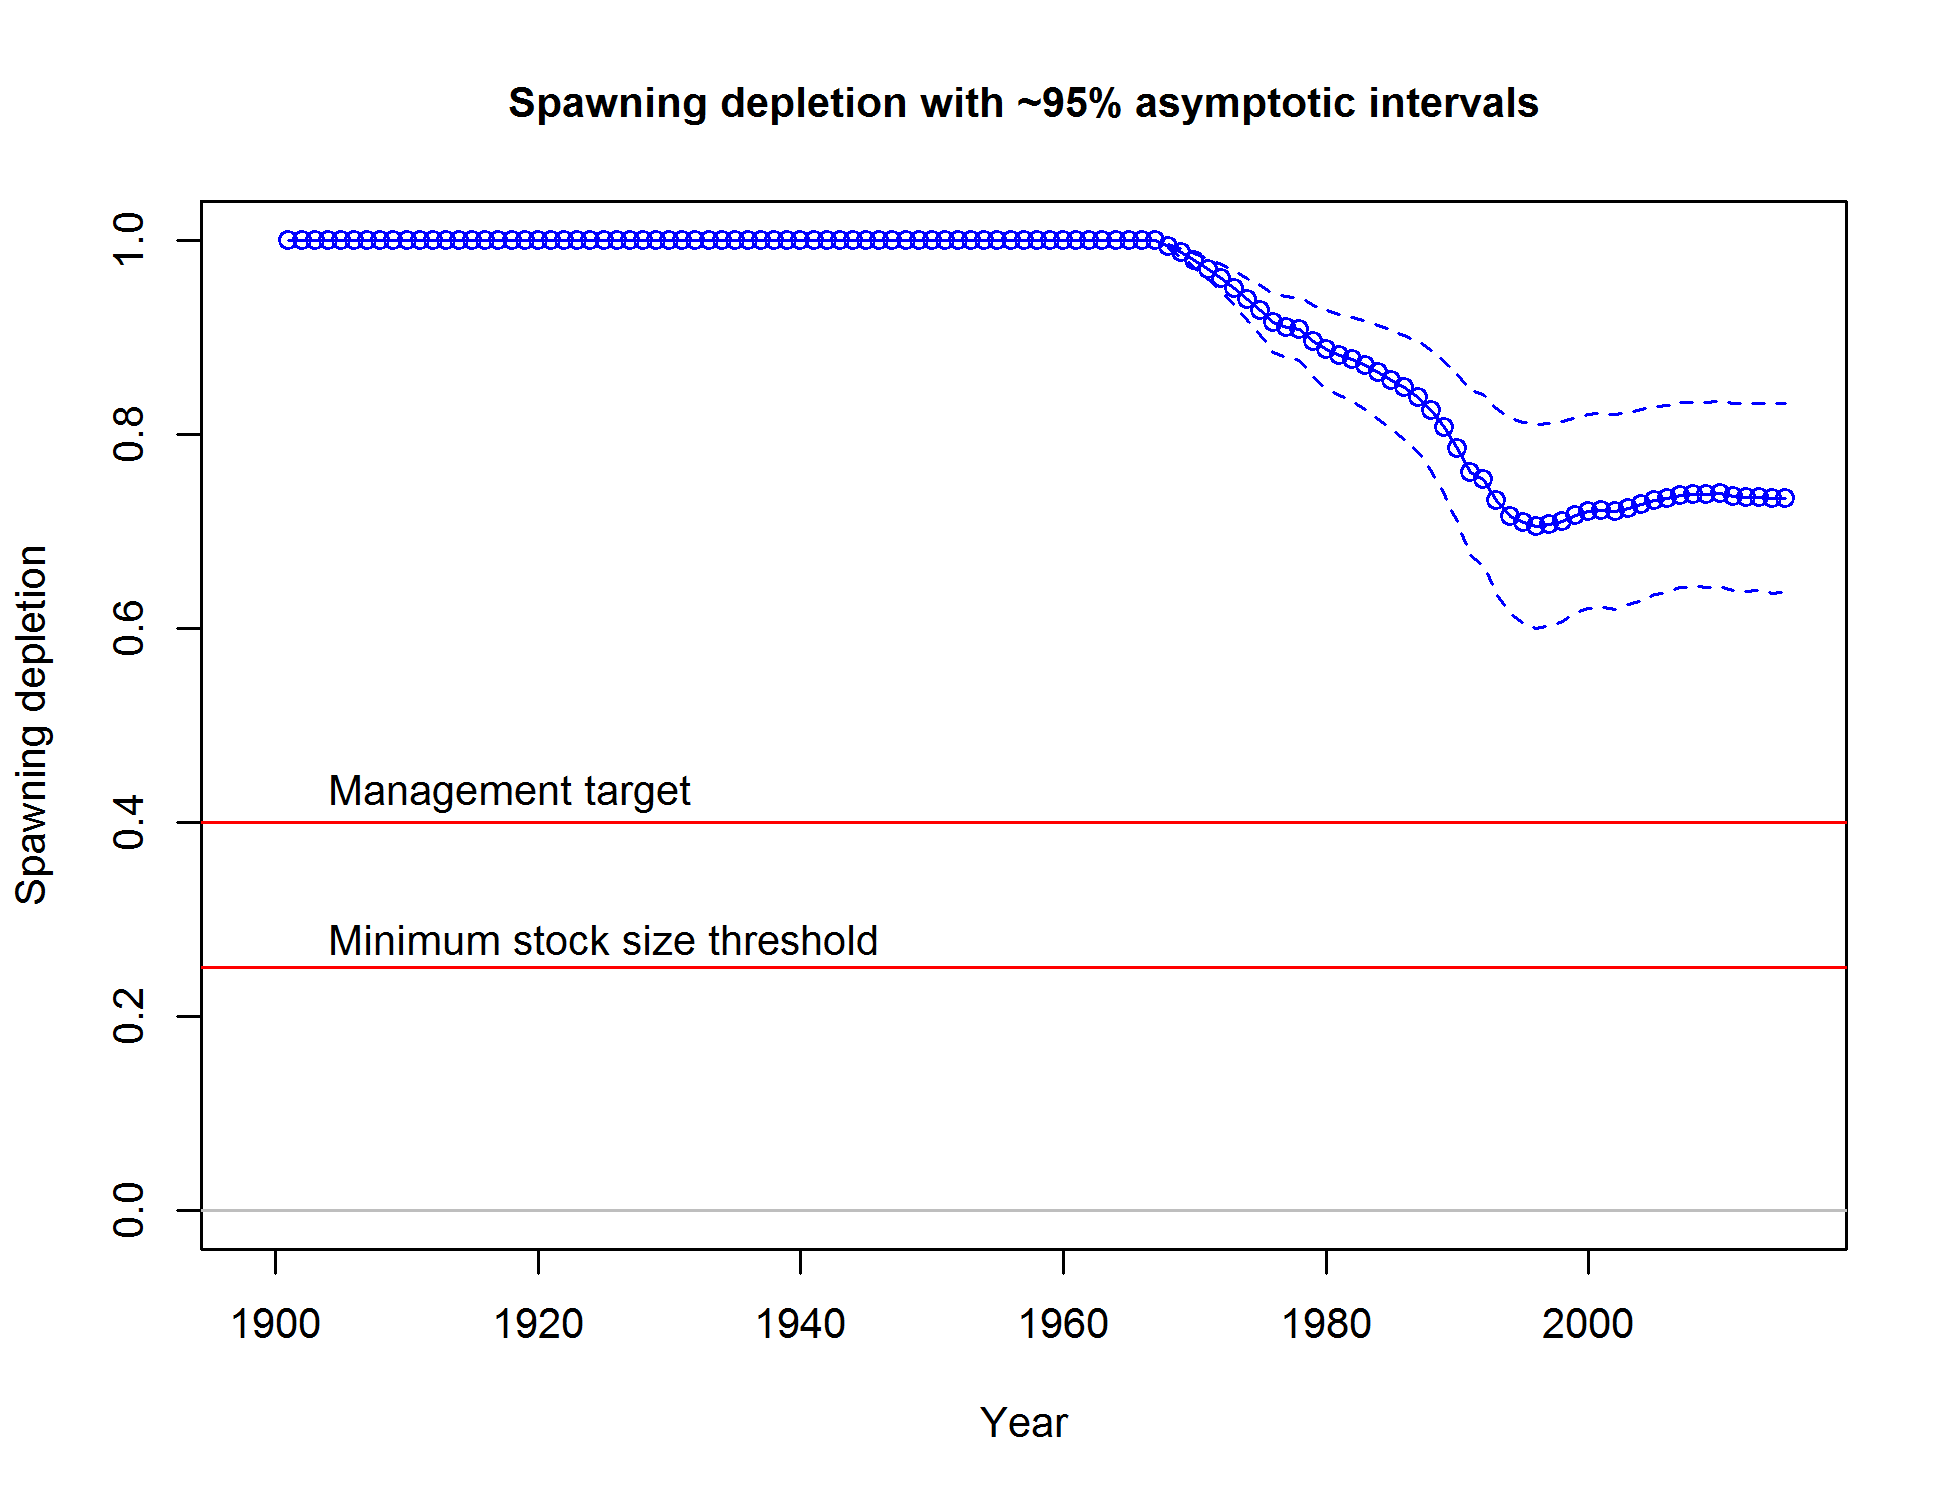
\includegraphics{r4ss/plots_mod1/ts9_Spawning_depletion_with_95_asymptotic_intervals_intervals.png}
\caption{Estimated relative depletion with approximate 95\% asymptotic
confidnce intervals (dashed lines) for the base case assessment model.
\label{fig:RelDeplete_all}}
\end{figure}

\FloatBarrier

\subsection*{Recruitment}\label{recruitment}
\addcontentsline{toc}{subsection}{Recruitment}

\hl{Include: trends and current levels relative to virgin or historic levels-include 
table for last 10 years and graph with long term estimates.}

Recruitment Figure: (Figure \ref{fig:Recruits_all})\\
Recruitment Tables: (Tables \ref{tab:Recruit_mod1})

\begin{table}[ht]
\centering
\caption{Recent estimated trend in recruitment with approximate 95% 
                                        confidence intervals determined from the base model} 
\label{tab:Recruit_mod1}
\begin{tabular}{>{\centering}p{.8in}>{\centering}p{1.0in}>{\centering}p{1.4in}>{\centering}p{1.0in}>{\centering}p{1.4in}}
  \hline
Year & Estimated Recruitment & \~{} 95\% confidence interval & Estimated Recruitment Devs. & \~{} 95\% confidence interval \\ 
  \hline
2008 & 70862.00 & 17357 - 289304 & 2.98 & 2.605 - 3.358 \\ 
  2009 & 1947.00 & 414 - 9162 & -0.67 & -1.598 - 0.261 \\ 
  2010 & 3171.00 & 642 - 15655 & -0.23 & -1.319 - 0.862 \\ 
  2011 & 4069.00 & 826 - 20047 & -0.02 & -1.090 - 1.045 \\ 
  2012 & 3956.00 & 781 - 20047 & -0.09 & -1.262 - 1.075 \\ 
  2013 & 5973.00 & 1159 - 30775 & 0.27 & -0.973 - 1.520 \\ 
  2014 & 4345.00 & 852 - 22172 & -0.12 & -1.383 - 1.150 \\ 
  2015 & 5358.00 & 1046 - 27437 & -0.00 & -1.372 - 1.372 \\ 
  2016 & 5888.00 & 1193 - 29070 & 0.00 & -1.372 - 1.372 \\ 
  2017 & 6312.00 & 1575 - 25298 & 0.00 & -0.970 - 0.970 \\ 
   \hline
\end{tabular}
\end{table}

\FloatBarrier

\begin{figure}
\centering
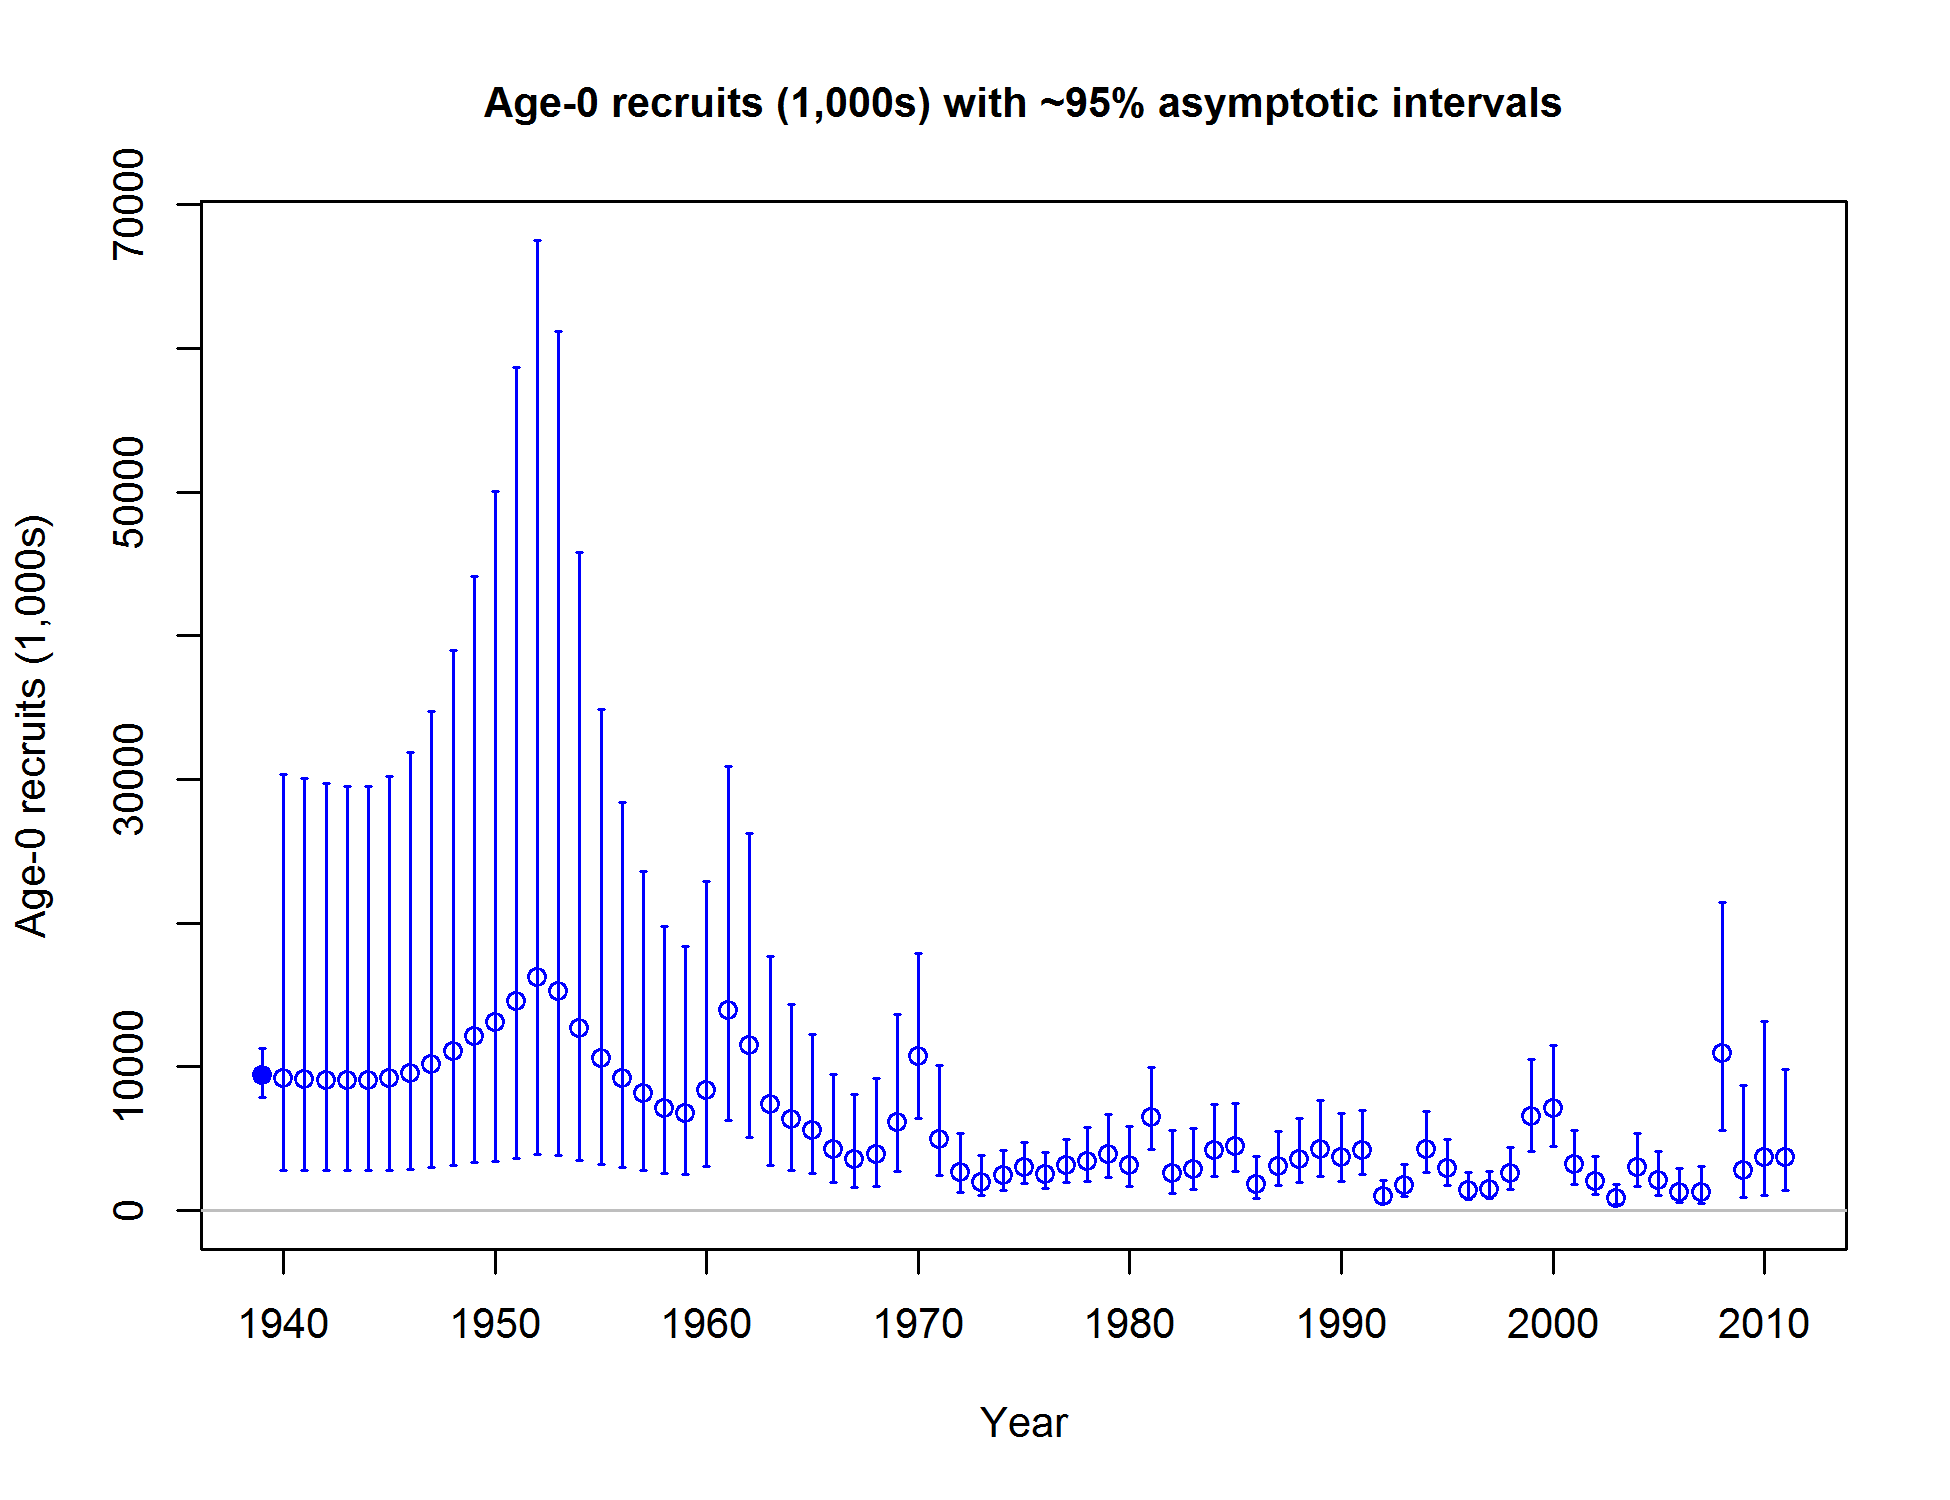
\includegraphics{r4ss/plots_mod1/ts11_Age-0_recruits_(1000s)_with_95_asymptotic_intervals.png}
\caption{Time series of estimated Pacific ocean perch recruitments for
the base-case model with 95\% confidence or credibility intervals.
\label{fig:Recruits_all}}
\end{figure}

\FloatBarrier

\subsection*{Exploitation status}\label{exploitation-status}
\addcontentsline{toc}{subsection}{Exploitation status}

\hl{Include: exploitation rates (i.e., total catch divided by exploitable biomass, or the annual SPR harvest rate) – include a table with the last 10 years of data and a graph showing the trend in fishing mortality relative to the target (y-axis) plotted against the trend in biomass relative to the target (x-axis).}

Exploitation Tables: Table \ref{tab:SPR_Exploit_mod1}, Table
\ref{tab:SPR_Exploit_mod2}, Table \ref{tab:SPR_Exploit_mod3}
Exploitation Figure: Figure \ref{fig:SPR_all}).

A summary of Pacific ocean perch exploitation histories for base model
is provided as Figure \ref{fig:Phase_all}.

\FloatBarrier

\begin{table}[ht]
\centering
\caption{Recent trend in spawning potential 
                                        ratio (1-SPR) and summary exploitation rate forPacific ocean perch.} 
\label{tab:SPR_Exploit_mod1}
\begin{tabular}{l>{\centering}p{1in}>{\centering}p{1.2in}>{\centering}p{1in}>{\centering}p{1.2in}}
  \hline
Year & Fishing intensity & \~{} 95\% confidence interval & Exploitation rate & \~{} 95\% confidence interval \\ 
  \hline
2007 & 0.279 & -0.097 - 0.655 & 0.006 & -0.003 - 0.015 \\ 
  2008 & 0.257 & -0.096 - 0.611 & 0.005 & -0.003 - 0.014 \\ 
  2009 & 0.266 & -0.101 - 0.633 & 0.006 & -0.003 - 0.015 \\ 
  2010 & 0.250 & -0.099 - 0.598 & 0.006 & -0.003 - 0.014 \\ 
  2011 & 0.099 & -0.049 - 0.247 & 0.002 & -0.001 - 0.004 \\ 
  2012 & 0.090 & -0.045 - 0.226 & 0.001 & -0.001 - 0.004 \\ 
  2013 & 0.083 & -0.042 - 0.208 & 0.001 & -0.001 - 0.003 \\ 
  2014 & 0.071 & -0.037 - 0.178 & 0.001 & -0.001 - 0.003 \\ 
  2015 & 0.068 & -0.036 - 0.172 & 0.001 & -0.001 - 0.003 \\ 
  2016 & 0.058 & -0.032 - 0.149 & 0.001 & -0.001 - 0.003 \\ 
   \hline
\end{tabular}
\end{table}

\FloatBarrier

\begin{figure}
\centering
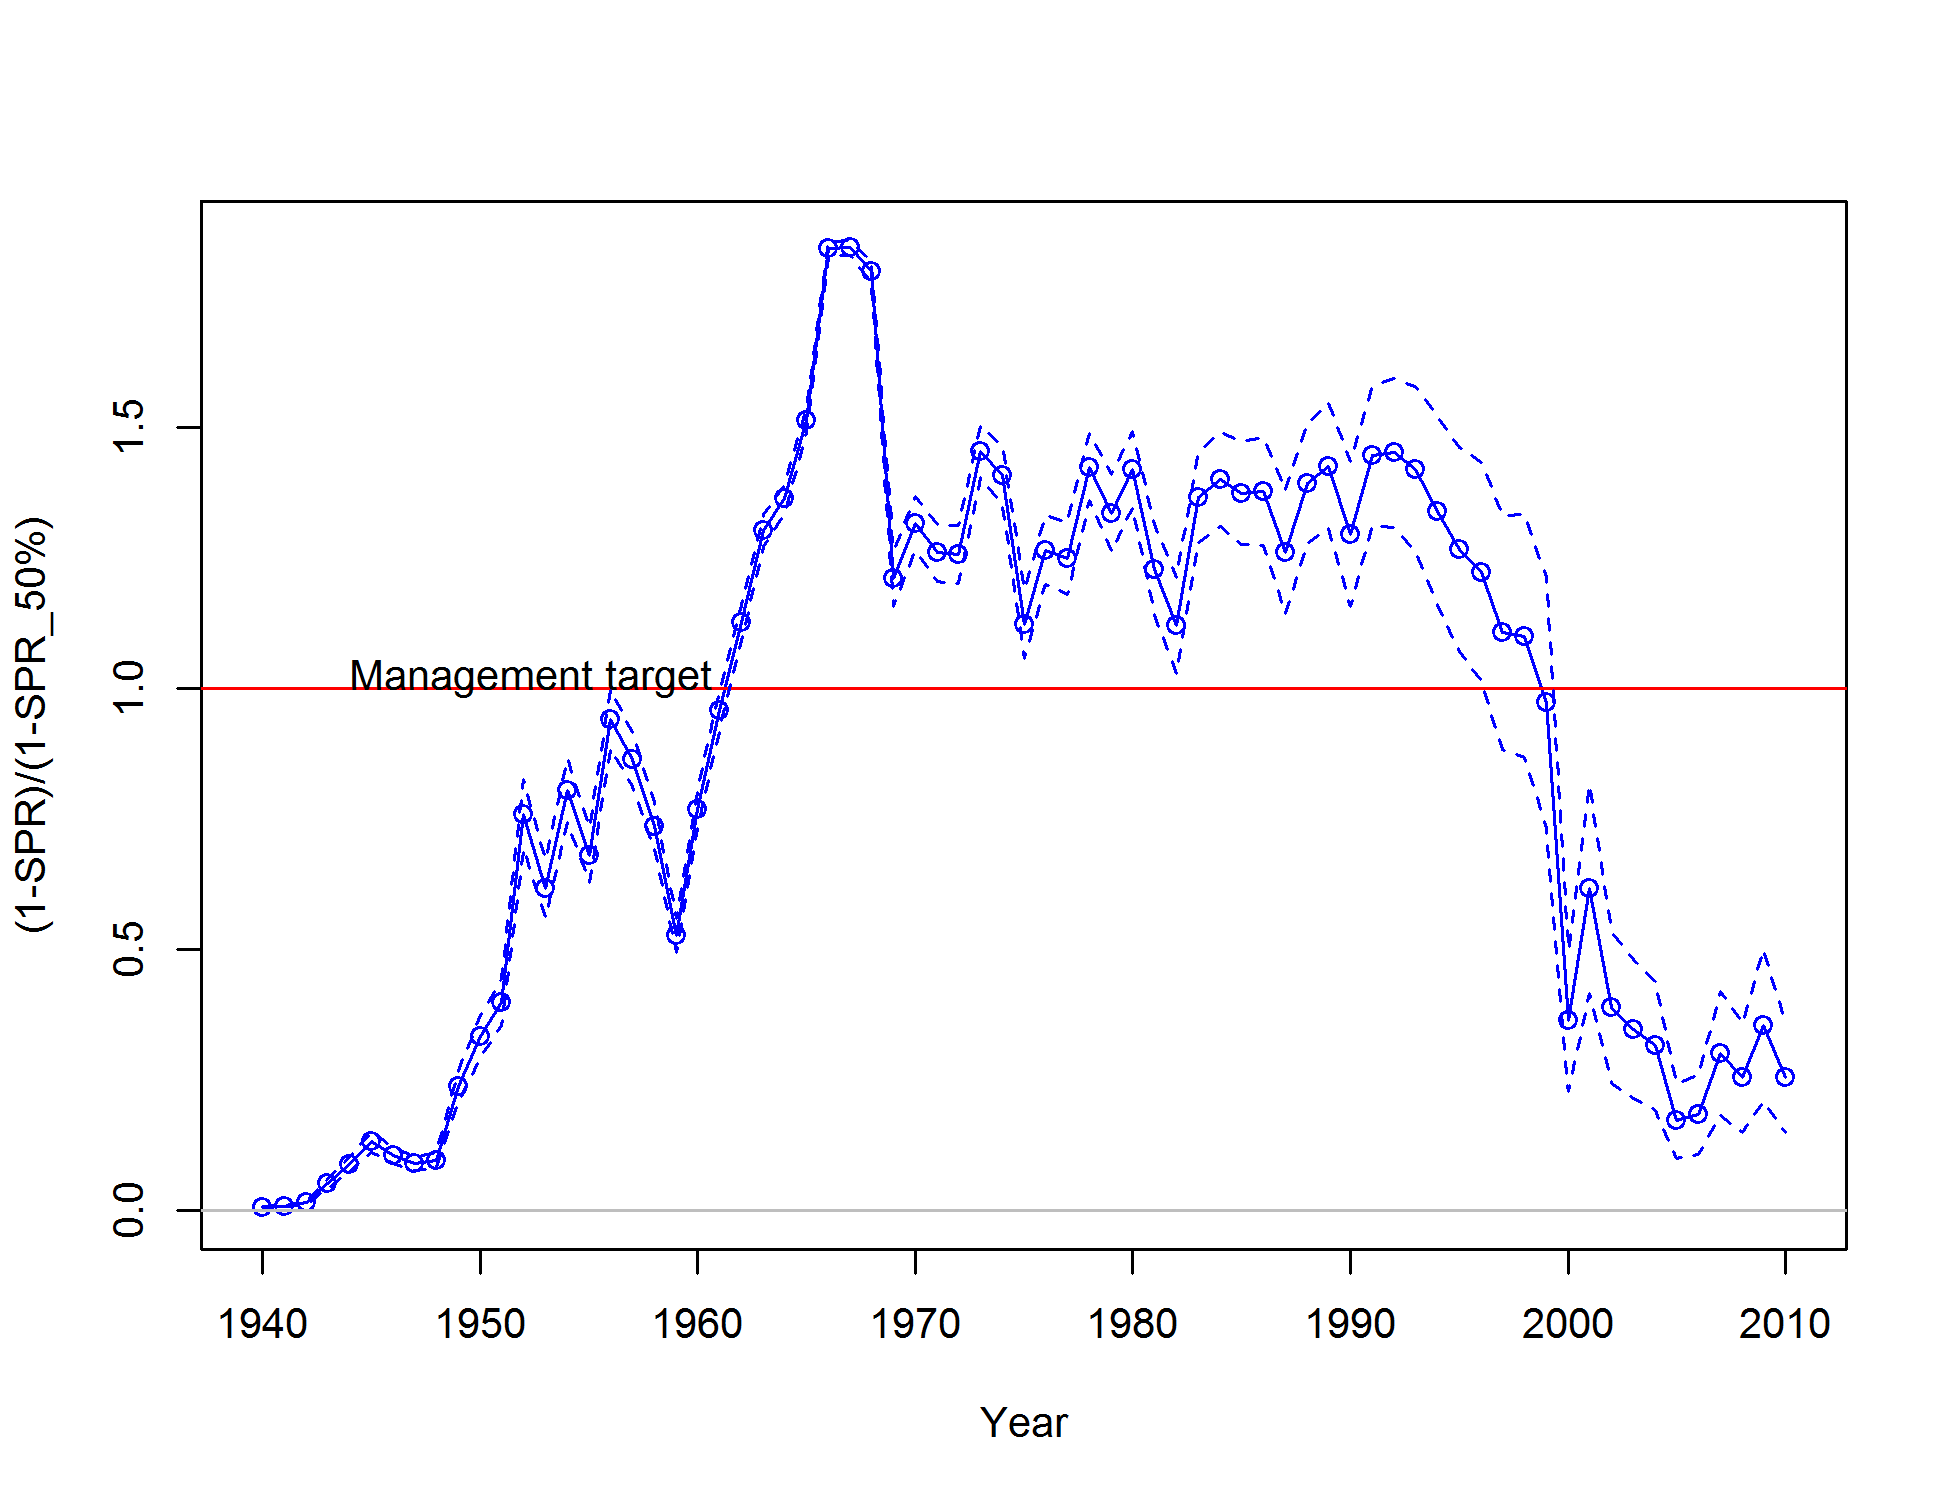
\includegraphics{r4ss/plots_mod1/SPR3_ratiointerval.png}
\caption{Estimated spawning potential ratio (SPR) for the base-case
model. One minus SPR is plotted so that higher exploitation rates occur
on the upper portion of the y-axis. The management target is plotted as
a red horizontal line and values above this reflect harvests in excess
of the overfishing proxy based on the SPR\textsubscript{50\%} harvest
rate. The last year in the time series is 2016. \label{fig:SPR_all}}
\end{figure}

\begin{figure}
\centering
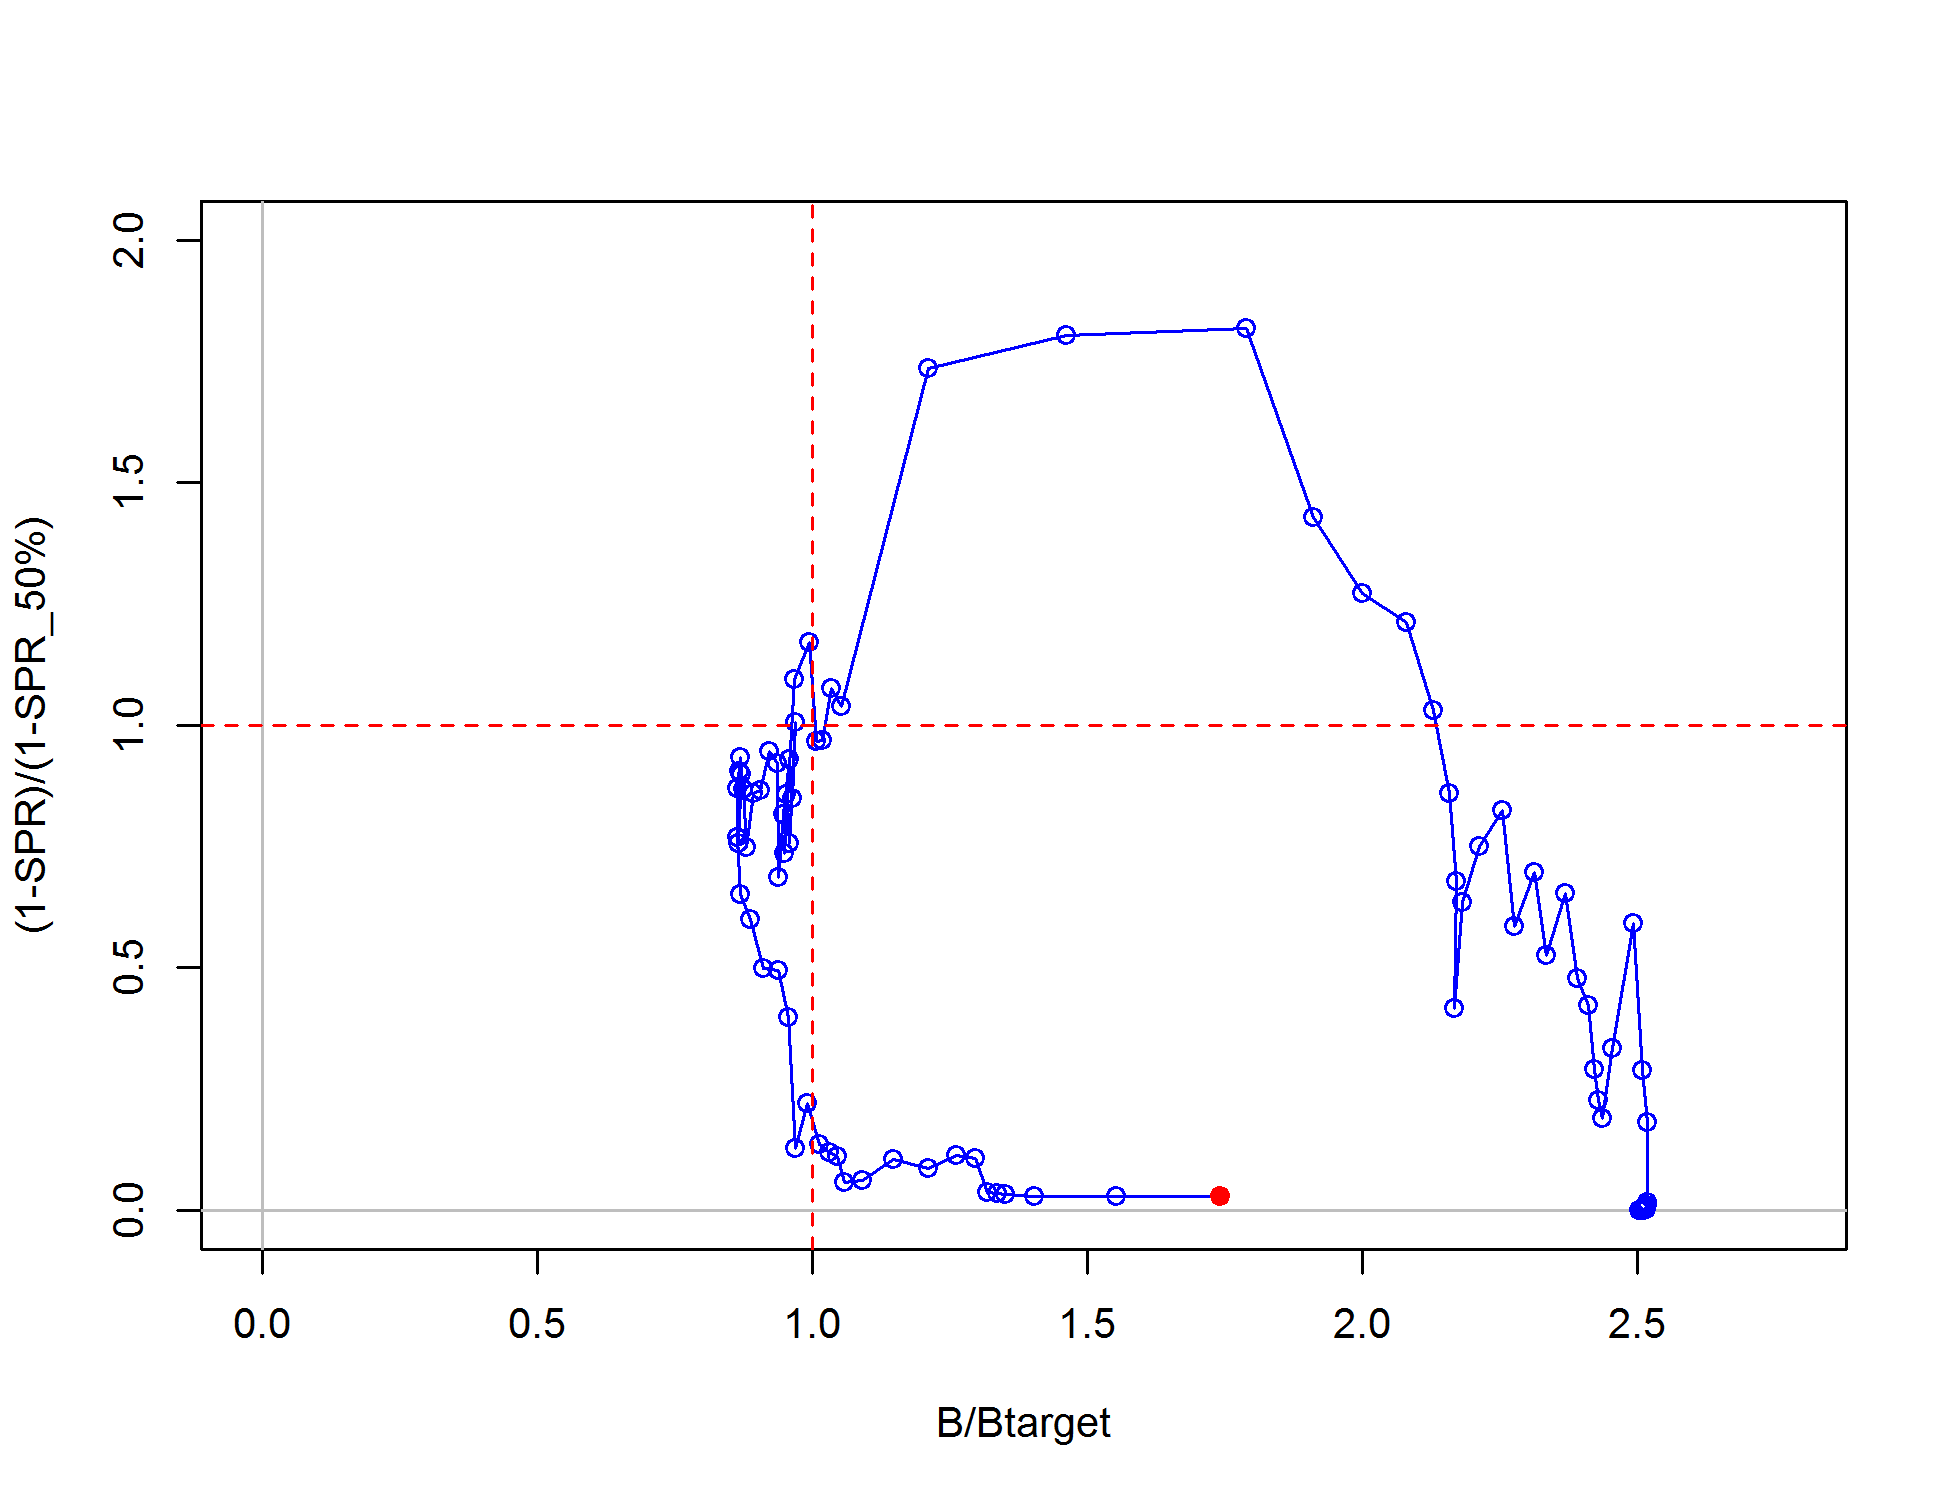
\includegraphics{r4ss/plots_mod1/SPR4_phase.png}
\caption{Phase plot of estimated relative (1-SPR) vs.~relative spawning
biomass for the base case model. The relative (1-SPR) is (1-SPR) divided
by 50\% (the SPR target). Relative depletion is the annual spawning
biomass divided by the unfished spawning biomass. \label{fig:Phase_all}}
\end{figure}

\FloatBarrier

\subsection*{Ecosystem Considerations}\label{ecosystem-considerations}
\addcontentsline{toc}{subsection}{Ecosystem Considerations}

In this assessment, ecosystem considerations were\ldots{}..

\subsection*{Reference Points}\label{reference-points}
\addcontentsline{toc}{subsection}{Reference Points}

\hl{Include:} management targets and definition of overfishing,
including the harvest rate that brings the stock to equilibrium at
\(B_{40\%}\) (the \(B_{MSY}\) proxy) and the equilibrium stock size that
results from fishing at the default harvest rate (the \(F_{MSY}\)
proxy). Include a summary table that compares estimated reference points
for SSB, SPR, Exploitation Rate and Yield based on SSBproxy for MSY,
SPRproxy for MSY, and estimated MSY values

\hl{Write intro paragraph}

This stock assessment estimates that Pacific ocean perch in the Base
model are below the biomass target, but above the minimum stock size
threshold. \hl{Add sentence about spawning output trend.} The estimated
relative depletion level for \hl{Model 1} in 2017 is 38\%
(\textasciitilde{}95\% asymptotic interval: \(\pm\) -18.2\%-94.1\%,
corresponding to an unfished spawning output of 2151 million eggs
(\textasciitilde{}95\% asymptotic interval:
-1245.35559241101-5547.095592411 million eggs) of spawning output in the
base model (Table \ref{tab:Ref_pts_mod1}). Unfished age 3+ biomass was
estimated to be 122166 mt in the base case model. The target spawning
output based on the biomass target (\(SB_{40\%}\)) is 2265.8 million
eggs, which gives a catch of 1176.1 mt. Equilibrium yield at the proxy
\(F_{MSY}\) harvest rate corresponding to \(SPR_{50\%}\) is 1018 mt.

\FloatBarrier

\begin{table}[ht]
\centering
\caption{Summary of reference 
                                      points and management quantities for the 
                                      base case.} 
\label{tab:Ref_pts_mod1}
\begin{tabular}{>{\raggedright}p{4.1in}>{\centering}p{.65in}>{\centering}p{1.4in}}
  \hline
\textbf{Quantity} & \textbf{Estimate} & \textbf{\~95\%  Confidence Interval} \\ 
  \hline
Unfished spawning output (million eggs) & 5664.4 &    4293.9 -   7034.9 \\ 
  Unfished age 3+ biomass (mt) & 122166 &   94382.3 - 149949.7 \\ 
  Unfished recruitment (R0, thousands) & 10014.3 &    7894.9 -  12702.7 \\ 
  Spawning output(2017 million eggs) & 2150.9 & -1245.356 -   5547.1 \\ 
  Depletion (2017) & 0.38 &    -0.182 -    0.941 \\ 
  \textbf{$\text{Reference points based on } \mathbf{SB_{40\%}}$} &  &  \\ 
  Proxy spawning output ($B_{40\%}$) & 2265.8 &    1717.6 -     2814 \\ 
  SPR resulting in $B_{40\%}$ ($SPR_{B40\%}$) & 0.615 &     0.443 -    0.788 \\ 
  Exploitation rate resulting in $B_{40\%}$ & 0.022 &     0.008 -    0.036 \\ 
  Yield with $SPR_{B40\%}$ at $B_{40\%}$ (mt) & 1176.1 &     287.7 -   2064.5 \\ 
  \textbf{\textit{Reference points based on SPR proxy for MSY}} &  &  \\ 
  Spawning output & 1245 &  -785.915 -   3275.9 \\ 
  $SPR_{proxy}$ & 0.5 &  \\ 
  Exploitation rate corresponding to $SPR_{proxy}$ & 0.033 &     0.033 -    0.034 \\ 
  Yield with $SPR_{proxy}$ at $SB_{SPR}$ (mt) & 1018 &  -630.883 -   2666.8 \\ 
  \textbf{\textit{Reference points based on estimated MSY values}} &  &  \\ 
  Spawning output at $MSY$ ($SB_{MSY}$) & 2176.7 &    1496.9 -   2856.5 \\ 
  $SPR_{MSY}$ & 0.605 &     0.374 -    0.837 \\ 
  Exploitation rate at $MSY$ & 0.023 &     0.003 -    0.043 \\ 
  $MSY$ (mt)  & 1177.3 &     275.5 -   2079.1 \\ 
   \hline
\end{tabular}
\end{table}

\FloatBarrier

\subsection*{Management Performance}\label{management-performance}
\addcontentsline{toc}{subsection}{Management Performance}

\hl{Include: catches in comparison to OFL, ABC and OY/ACL values for the most 
recent 10 years (when available), overfishing levels, actual catch and discard. 
Include OFL(encountered), OFL(retained) and OFL(dead) if different due to discard 
and discard mortality.}

Management performance table: Table \ref{tab:mnmgt_perform}

\begin{table}[ht]
\centering
\caption{Recent trend in total catch and commercial 
                              landings (mt) relative to the management guidelines. 
                              Estimated total catch reflect the commercial landings 
                              plus the model estimated discarded biomass.} 
\label{tab:mnmgt_perform}
\scalebox{0.9}{
\begin{tabular}{>{\raggedleft}p{0.5in}>{\centering}p{1.1in}>{\centering}p{1.1in}>{\centering}p{1.1in}>{\centering}p{1.1in}>{\centering}p{1.1in}}
  \hline
Year & OFL (mt; ABC prior to 2011) & ABC (mt) & ACL (mt; OY prior to 2011) & Total landings (mt) & Estimated total catch (mt) \\ 
  \hline
\text{2007} & - & - & 150 & 134 & 158 \\ 
  \text{2008} & - & - & 150 & 92 & 151 \\ 
  \text{2009} & - & - & 189 & 97 & 169 \\ 
  \text{2010} & - & - & 200 & 99 & 161 \\ 
  \text{2011} & - & - & 180 & 61 & 61 \\ 
  \text{2012} & - & - & 183 & 59 & 59 \\ 
  \text{2013} & - & - & 150 & 57 & 58 \\ 
  \text{2014} & - & - & 153 & 54 & 55 \\ 
  \text{2015} & - & - & 158 & 60 & 60 \\ 
  \text{2016} & - & - & 164 & 58 & 58 \\ 
   \hline
\end{tabular}
}
\end{table}

\subsection*{Unresolved Problems And Major
Uncertainties}\label{unresolved-problems-and-major-uncertainties}
\addcontentsline{toc}{subsection}{Unresolved Problems And Major
Uncertainties}

TBD after STAR panel

\FloatBarrier

\subsection*{Decision Table(s) (groundfish
only)}\label{decision-tables-groundfish-only}
\addcontentsline{toc}{subsection}{Decision Table(s) (groundfish only)}

\hl{Include: projected yields (OFL, ABC and ACL), spawning biomass, and stock 
depletion levels for each year. Not required in draft assessments undergoing review.}

OFL projection table: Table \ref{tab:OFL_projection}

Decision table(s) Table \ref{tab:Decision_table_mod1}, Table
\ref{tab:Decision_table_mod2}, Table \ref{tab:Decision_table_mod3}

\begin{verbatim}
Yield curve: Figure \ref{fig:Yield_all}
\end{verbatim}

\begin{table}[ht]
\centering
\caption{Projections of potential OFL (mt) and ACL (mt) and the estimated spawning output and relative biomass.} 
\label{tab:OFL_projection}
\begin{tabular}{lllll}
  \hline
Year & OFL & ACL & Spawning Output ( million eggs ) & Relative Biomass \\ 
  \hline
2017 & 1899 & 1783 & 2151 & 0.380 \\ 
  2018 & 1988 & 1898 & 2257 & 0.398 \\ 
  2019 & 2018 & 1929 & 2312 & 0.408 \\ 
  2020 & 2008 & 1919 & 2337 & 0.413 \\ 
  2021 & 1975 & 1888 & 2342 & 0.413 \\ 
  2022 & 1935 & 1850 & 2333 & 0.412 \\ 
  2023 & 1894 & 1811 & 2316 & 0.409 \\ 
  2024 & 1858 & 1776 & 2296 & 0.405 \\ 
  2025 & 1827 & 1747 & 2274 & 0.402 \\ 
  2026 & 1801 & 1718 & 2252 & 0.398 \\ 
  2027 & 1779 & 1692 & 2230 & 0.394 \\ 
  2028 & 1760 & 1669 & 2210 & 0.390 \\ 
   \hline
\end{tabular}
\end{table}\begin{table}[ht]
\centering
\caption{Summary of 10-year 
                                             projections beginning in 2019 
                                             for alternate states of nature based on 
                                             an axis of uncertainty for the base model. 
                                             Columns range over low, mid, and high
                                             states of nature, and rows range over different 
                                             assumptions of catch levels. An entry of "--" 
                                             indicates that the stock is driven to very low 
                                             abundance under the particular scenario.} 
\label{tab:Decision_table_mod1}
\scalebox{0.85}{
\begin{tabular}{l|cc|>{\centering}p{.7in}c|>{\centering}p{.7in}c|>{\centering}p{.7in}c}
   \multicolumn{3}{c}{}  &  \multicolumn{2}{c}{} 
                               & \multicolumn{2}{c}{\textbf{States of nature}} 
                               & \multicolumn{2}{c}{} \\
  \multicolumn{3}{c}{}  &  \multicolumn{2}{c}{Low M 0.05} 
                               & \multicolumn{2}{c}{Base M 0.07} 
                               &  \multicolumn{2}{c}{High M 0.09} \\
 \hline
 & Year & Catch & Spawning Output & Depletion & Spawning Output & Depletion & Spawning Output & Depletion \\ 
  \hline
 & 2019 & - & - & - & - & - & - & - \\ 
   & 2020 & - & - & - & - & - & - & - \\ 
   & 2021 & - & - & - & - & - & - & - \\ 
  40-10 Rule,  & 2022 & - & - & - & - & - & - & - \\ 
  Low M & 2023 & - & - & - & - & - & - & - \\ 
   & 2024 & - & - & - & - & - & - & - \\ 
   & 2025 & - & - & - & - & - & - & - \\ 
   & 2026 & - & - & - & - & - & - & - \\ 
   & 2027 & - & - & - & - & - & - & - \\ 
   & 2028 & - & - & - & - & - & - & - \\ 
   \hline
 & 2019 & - & - & - & - & - & - & - \\ 
   & 2020 & - & - & - & - & - & - & - \\ 
   & 2021 & - & - & - & - & - & - & - \\ 
  40-10 Rule & 2022 & - & - & - & - & - & - & - \\ 
   & 2023 & - & - & - & - & - & - & - \\ 
   & 2024 & - & - & - & - & - & - & - \\ 
   & 2025 & - & - & - & - & - & - & - \\ 
   & 2026 & - & - & - & - & - & - & - \\ 
   & 2027 & - & - & - & - & - & - & - \\ 
   & 2028 & - & - & - & - & - & - & - \\ 
   \hline
 & 2019 & - & - & - & - & - & - & - \\ 
   & 2020 & - & - & - & - & - & - & - \\ 
   & 2021 & - & - & - & - & - & - & - \\ 
  40-10 Rule, & 2022 & - & - & - & - & - & - & - \\ 
  High M & 2023 & - & - & - & - & - & - & - \\ 
   & 2024 & - & - & - & - & - & - & - \\ 
   & 2025 & - & - & - & - & - & - & - \\ 
   & 2026 & - & - & - & - & - & - & - \\ 
   & 2027 & - & - & - & - & - & - & - \\ 
   & 2028 & - & - & - & - & - & - & - \\ 
   \hline
 & 2019 & - & - & - & - & - & - & - \\ 
   & 2020 & - & - & - & - & - & - & - \\ 
   & 2021 & - & - & - & - & - & - & - \\ 
  Average & 2022 & - & - & - & - & - & - & - \\ 
  Catch & 2023 & - & - & - & - & - & - & - \\ 
   & 2024 & - & - & - & - & - & - & - \\ 
   & 2025 & - & - & - & - & - & - & - \\ 
   & 2026 & - & - & - & - & - & - & - \\ 
   & 2027 & - & - & - & - & - & - & - \\ 
   & 2028 & - & - & - & - & - & - & - \\ 
   \hline
\end{tabular}
}
\end{table}

\begin{sidewaystable}[ht]
\centering
\caption{Base model results summary.} 
\label{tab:base_summary}
\scalebox{0.6}{
\begin{tabular}{r>{\centering}p{1.1in}>{\centering}p{1.1in}>{\centering}p{1.1in}>{\centering}p{1.1in}>{\centering}p{1.1in}>{\centering}p{1.1in}>{\centering}p{1.1in}>{\centering}p{1.1in}>{\centering}p{1.1in}>{\centering}p{1.1in}}
  \hline
Quantity & 2009 & 2010 & 2011 & 2012 & 2013 & 2014 & 2015 & 2016 & 2017 & 2018 \\ 
  \hline
Landings (mt) & - & - & - & - & - & - & - & - & - & - \\ 
  Total Est. Catch (mt) & 150 & 189 & 200 & 180 & 183 & 150 & 153 & 158 & 164 & 281 \\ 
  OFL (mt) & 92 & 97 & 99 & 61 & 59 & 57 & 54 & 60 & 58 &  \\ 
  ACL (mt) & 151 & 169 & 161 &  61 &  59 &  58 &  55 &  60 &  58 &  \\ 
   \hline
(1-$SPR$)(1-$SPR_{50\%}$) & 0.26 & 0.27 & 0.25 & 0.10 & 0.09 & 0.08 & 0.07 & 0.07 & 0.06 &  \\ 
   \hline
Exploitation rate & 0.01 & 0.01 & 0.01 & 0.00 & 0.00 & 0.00 & 0.00 & 0.00 & 0.00 &  \\ 
  Age 3+ biomass (mt) & 27737.5 & 28463.0 & 29077.8 & 37251.2 & 41154.9 & 44993.1 & 48570.4 & 51699.7 & 54560.3 & 56851.5 \\ 
   \hline
Spawning Output & 1100 & 1155 & 1203 & 1245 & 1288 & 1336 & 1442 & 1656 & 1919 & 2151 \\ 
  ~95\% CI & -590 - 2790 & -628 - 2939 & -664 - 3070 & -698 - 3189 & -726 - 3302 & -757 - 3429 & -820 - 3704 & -946 - 4258 & -1104 - 4942 & -1245 - 5547 \\ 
   \hline
Depletion & 0.194 & 0.204 & 0.212 & 0.220 & 0.227 & 0.236 & 0.255 & 0.292 & 0.339 & 0.380 \\ 
  ~95\% CI & -0.084 - 0.472 & -0.090 - 0.498 & -0.095 - 0.520 & -0.101 - 0.540 & -0.105 - 0.560 & -0.110 - 0.581 & -0.119 - 0.628 & -0.137 - 0.722 & -0.161 - 0.838 & -0.182 - 0.941 \\ 
   \hline
Recruits & 70862 &  1947 &  3171 &  4069 &  3956 &  5973 &  4345 &  5358 &  5888 &  6312 \\ 
  ~95\% CI & 17357 - 289304 & 414 - 9162 & 642 - 15655 & 826 - 20047 & 781 - 20047 & 1159 - 30775 & 852 - 22172 & 1046 - 27437 & 1193 - 29070 & 1575 - 25298 \\ 
   \hline
\end{tabular}
}
\end{sidewaystable}

\begin{figure}
\centering
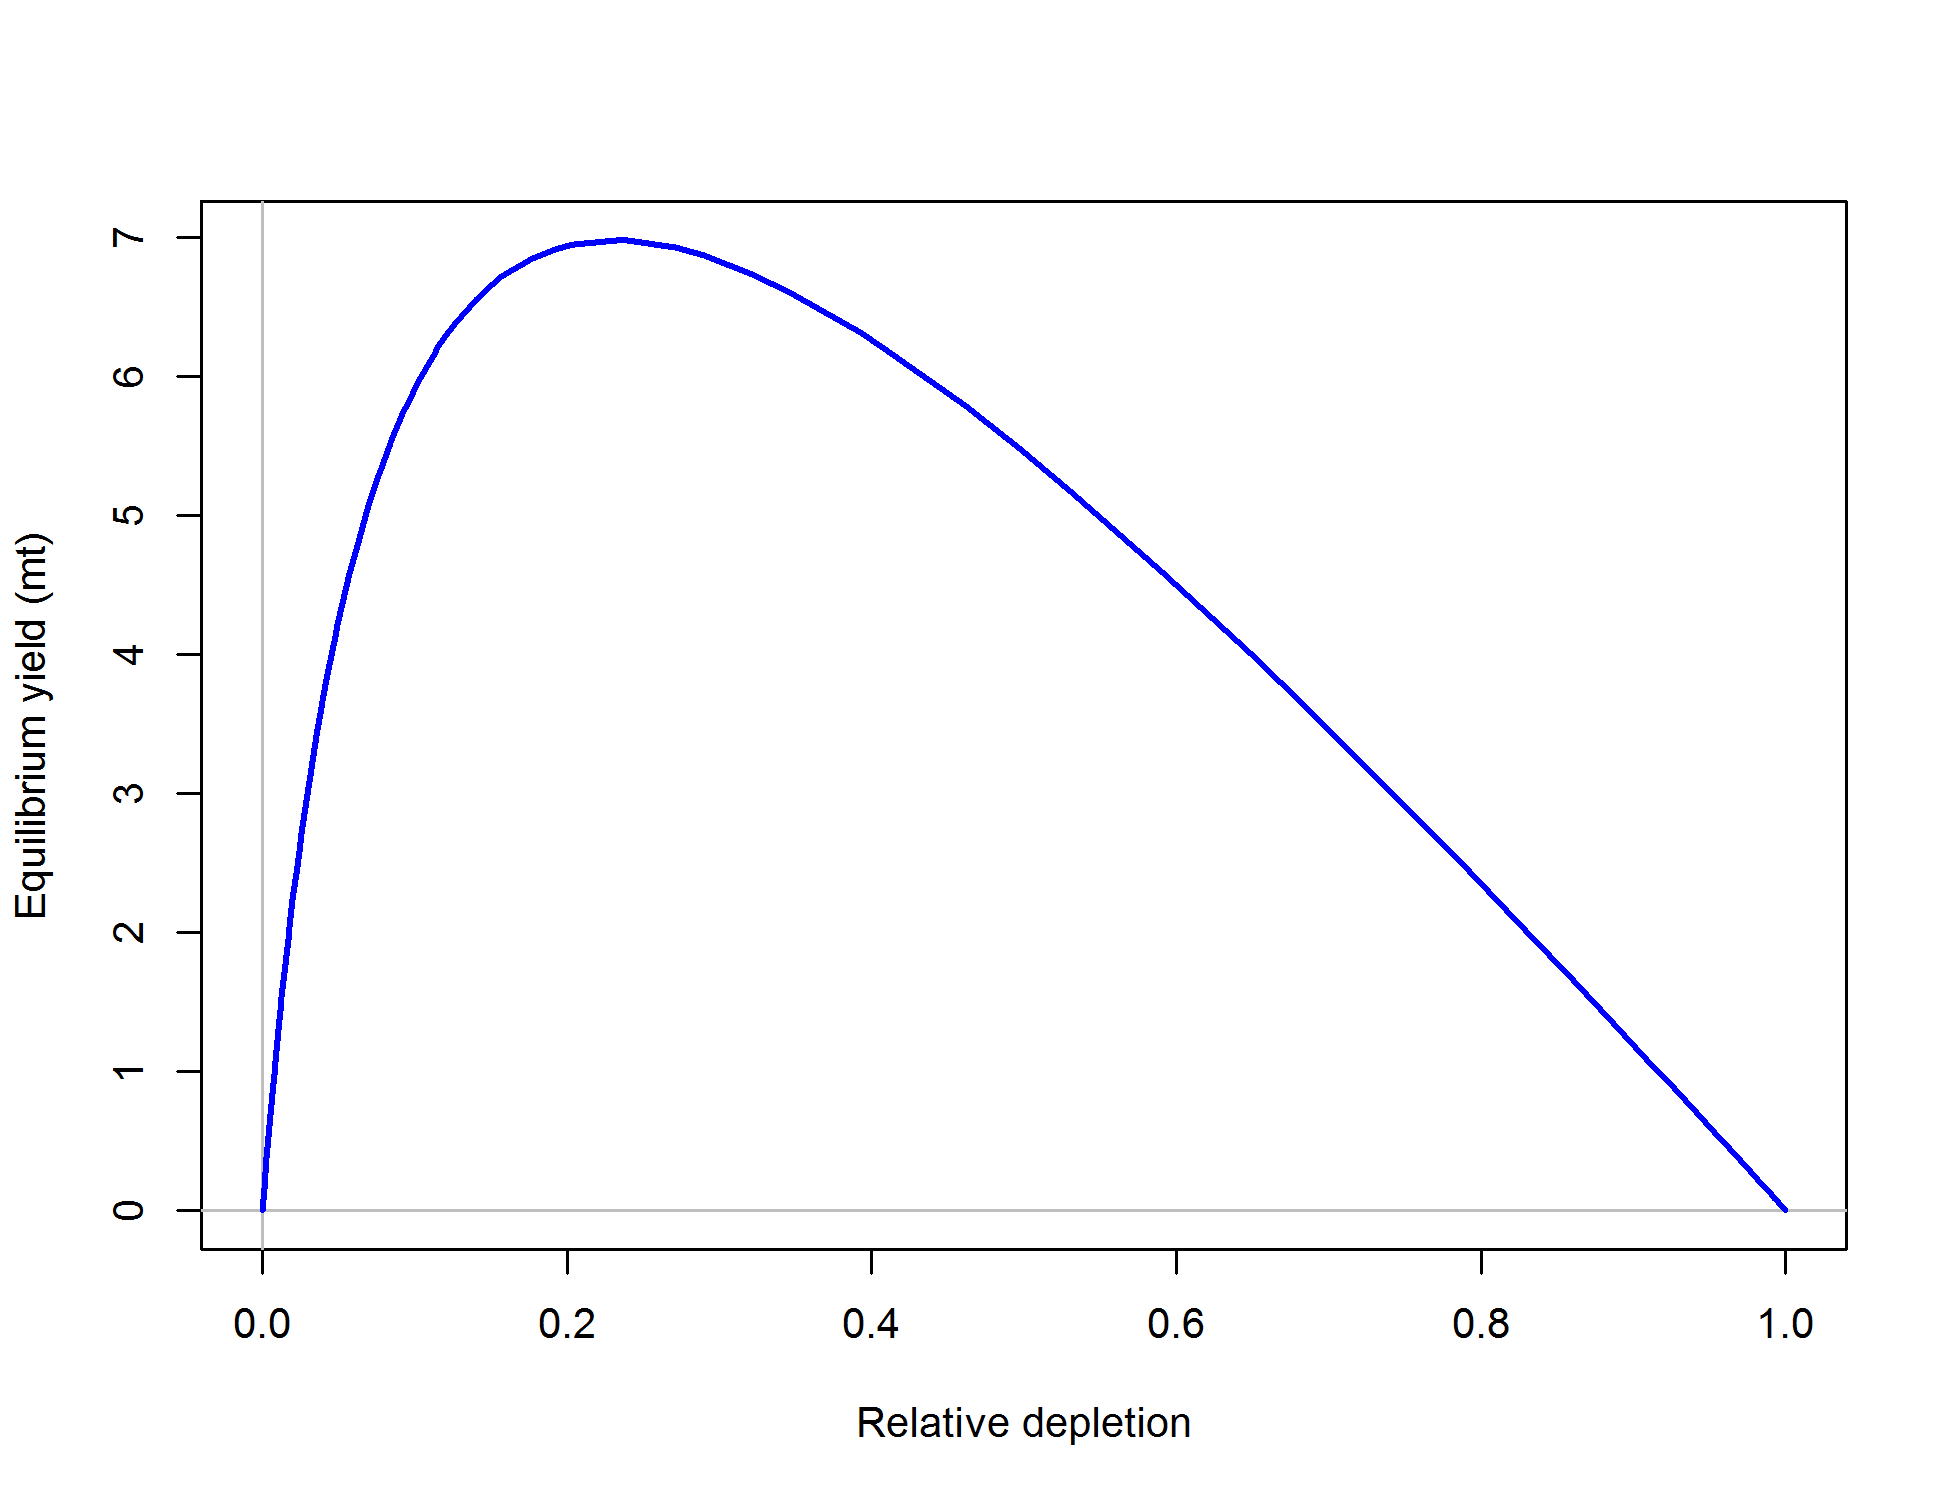
\includegraphics{r4ss/plots_mod1/yield1_yield_curve.png}
\caption{Equilibrium yield curve for the base case model. Values are
based on the 2016 fishery selectivity and with steepness fixed
at\ldots{} \label{fig:Yield_all}}
\end{figure}

\FloatBarrier

\newpage

\subsection*{Research And Data Needs}\label{research-and-data-needs}
\addcontentsline{toc}{subsection}{Research And Data Needs}

\hl{Include: identify information gaps that seriously impede the stock assessment.}

We recommend the following research be conducted before the next
assessment:

\begin{enumerate}

\item List item No. 1 in the list

\item List item No. 2 in the list, etc.

\end{enumerate}

\subsection*{Rebuilding Projections}\label{rebuilding-projections}
\addcontentsline{toc}{subsection}{Rebuilding Projections}

\hl{Include: reference to the principal results from rebuilding analysis if the 
stock is overfished. This section should be included in the Final/SAFE version 
assessment document but is not required for draft assessments undergoing review. 
See Rebuilding Analysis terms of reference for detailed information on 
rebuilding analysis requirements.}

\FloatBarrier

\newpage

\renewcommand{\thefigure}{\arabic{figure}}
\renewcommand{\thetable}{\arabic{table}}

\setcounter{figure}{0} \setcounter{table}{0}

\section{Introduction}\label{introduction}

\subsection{Basic Information}\label{basic-information}

Pacific ocean perch (\emph{Sebastes alutus}) are most abundant in the
Gulf of Alaska, and have been observed off of Japan, in the Bering Sea,
and south to Baja California, although they are sparse south of Oregon
and rare in southern California. While genetic studies have found three
populations of Pacific ocean perch off of British Columbia (Seeb and
Gunderson \protect\hyperlink{ref-seeb_genetic_1988}{1988}, Withler et
al. \protect\hyperlink{ref-withler_co-existing_2001}{2001}) with,
notably, a separate stock off of Vancouver Island, no significant
genetic differences have been found in the range covered by this
assessment. Pacific ocean perch show dimorphic growth, with females
reaching a slightly large size than males. Males and females are equally
abundant on rearing grounds at age 1.5.

The Pacific ocean perch population has been modeled as a single stock
off of the U.S. West Coast (essentially northern California to the
Canadian border, since Pacific ocean perch are seen extremely rarely in
central and southern California). Good recruitments show up in
size-composition data throughout all portions of this area, which
supports the single stock hypothesis. This assessment includes landings
and catch data for Pacific ocean perch from the states of Washington,
Oregon and California, along with records from foreign fisheries, the
at-sea hake fleet, and surveys.

Prior to 1966, the Pacific ocean perch resource off of the northern
portion of the U.S. West Coast was harvested almost entirely by Canadian
and United States vessels. Harvest was negligible prior to 1940, reached
1,300 mt in 1950, 3,200 mt in 1961 and exceeded 7,600 mt in 1965.
Catches increased dramatically after 1965, with the introduction of
large distant-water fishing fleets from the Soviet Union and Japan. Both
nations employed large factory stern trawlers as their primary method
for harvesting Pacific ocean perch. Peak removals by all foreign nations
combined are estimated at over 15,000 mt in 1966 and remained over
12,000 mt in 1967. These numbers are based upon a re-analysis of the
foreign catch data (Rogers
\protect\hyperlink{ref-rogers_species_2003}{2003}), which focused on
deriving a more realistic species composition for catches previously
identified only as Pacific ocean perch. Catches declined rapidly
following these peak years, and Pacific ocean perch stocks were
considered to be severely depleted throughout the Oregon-Vancouver
Island region by 1969 (Gunderson
\protect\hyperlink{ref-gunderson_population_1977}{1977}, Gunderson et
al. \protect\hyperlink{ref-gunderson_status_1977}{1977}). Landed harvest
averaged 1,350 mt over the period 1977-94. Landings have continued to
decline since 1994, primarily due to more restrictive management.

Prior to 1977, Pacific ocean perch in the northeast Pacific were managed
by the Canadian Government in its waters and by the individual states in
waters off of the United States. With implementation of the Magnuson
Fishery Conservation and Management Act (MFCMA) in 1977, U.S.
territorial waters were extended to 200 miles from shore, and primary
responsibility for management of the groundfish stocks off Washington,
Oregon and California shifted from the states to the Pacific Fishery
Management Council (PFMC) and the National Marine Fisheries Service
(NMFS). At that time, however, a Fishery Management Plan (FMP) for the
west coast groundfish stocks had not yet been approved. In the interim,
the state agencies worked with the PFMC to address conservation issues.
In 1981, the PFMC adopted a management strategy to rebuild the depleted
Pacific ocean perch stocks to levels that would produce Maximum
Sustainable Yield (MSY) within 20 years. On the basis of cohort analysis
(Gunderson \protect\hyperlink{ref-gunderson_results_1978}{1978}), the
PFMC set Acceptable Biological Catch (ABC) levels at 600 mt for the US
portion of the Vancouver INPFC area and 950 mt for the Columbia INPFC
area. To implement this strategy, the states of Oregon and Washington
each established landing limits for Pacific ocean perch. Trawl trip
limits of various forms remained in effect through 2010 (\hl{Table 1}).

Age estimates for Pacific ocean perch prior to the 1980s were made via
surface ageing of otoliths, which misses the very tight annuli at the
edge of the otolith once the fish reaches near maximum size. Ages are
biased by around age 10-12, and maximum age was estimated to be in the
20s, which lead to an overestimate of the natural mortality rate and the
productivity of the stock. Using break and burn methods, Pacific ocean
perch have been aged to over 100 years, and we now know that the
underlying assumptions of the early models were overly optimistic about
productivity. Research surveys have been used to provide
fishery-independent information about the abundance, distribution, and
biological characteristics of Pacific ocean perch. A coast-wide survey
of the rockfish resource was conducted in 1977 (Gunderson and Sample
\protect\hyperlink{ref-gunderson_distribution_1980}{1980}) and was
repeated every three years through 2004 (referred to as the `Triennial
Survey'). The National Marine Fisheries Service (NMFS) coordinated a
cooperative research survey of the Pacific ocean perch stocks off
Washington and Oregon with the Washington Department of Fisheries (WDFW)
and the Oregon Department of Fish and Wildlife (ODFW) in March-May 1979
(Wilkins and Golden
\protect\hyperlink{ref-wilkins_condition_1983}{1983}). This survey was
repeated in 1985 (referred to as the Pacific ocean perch Survey). Two
slope surveys have been conducted on the West Coast in recent years, one
using the research vessel Miller Freeman, which ended in 2001 (referred
to as the `AFSC Slope Survey'), and another ongoing cooperative survey
using commercial fishing vessels which began in 1998 as a DTS (Dover
sole, thornyhead and sablefish) survey, was expanded to other groundfish
in 1999 (referred to as the `NWFSC Slope Survey'). In 2003, this survey
was expanded spatially to include the shelf. This last survey, conducted
by the NWFSC, continues to cover depths from 30-700 fathoms (55-1280
meters) on an annual basis (referred to as the `NWFSC shelf-slope
Survey').

\subsection{Map}\label{map}

A map showing the scope of the assessment and depicting boundaries for
fisheries or data collection strata is provided in Figure
\ref{fig:boundary_map}.

\subsection{Life History and Ecosystem
Considerations}\label{life-history-and-ecosystem-considerations}

\hl{Include: Ecosystem considerations (e.g., ecosystem role and trophic relationships of  the species, habitat requirements/preferences, relevant data on ecosystem processes  that may affect stock or parameters used in the stock assessment, and/or cross-FMP  interactions with other fisheries). This section should note if environmental  correlations or food web interactions were incorporated into the assessment model.  The length and depth of this section would depend on availability of data and reports  from the IEA, expertise of the STAT, and whether ecosystem factors are informational  to contribute quantitative information to the assessment.}

\subsection{Fishery Information}\label{fishery-information}

\hl{Include: Important features of current fishery and relevant history of fishery.}

\subsection{Summary of Management
History}\label{summary-of-management-history}

\hl{Include: Summary of management history (e.g., changes in mesh sizes, trip 
                                            limits, or other management actions that may have significantly altered selection, 
                                            catch rates, or discards).}

\subsection{Management Performance}\label{management-performance-1}

\hl{Include: Management performance, including a table or tables comparing 
  Overfishing Limit (OFL), Annual Catch Limit (ACL), Harvest Guideline (HG) 
  [CPS only], landings, and catch (i.e., landings plus discard) for each area and year.}

Management performance table: (Table \ref{tab:mnmgt_perform})\\
A summary of these values as well as other base case summary results can
be found in Table \ref{tab:base_summary}.

\subsection{Fisheries off Canada, Alaska, and/or
Mexico}\label{fisheries-off-canada-alaska-andor-mexico}

Include if necessary.

\section{Assessment}\label{assessment}

\subsection{Data}\label{data}

Data used in the Pacific ocean perch assessment are summarized in Figure
\ref{fig:data_plot}. A description of each data source is provided
below.

\subsubsection{Commercial Fishery
Landings}\label{commercial-fishery-landings}

\textbf{Washington}

Historical commercial fishery landigns of Pacific ocean perch from
Washington for the years 1918-2016 were obtained from Theresa Tsou
(WDFW) and Phillip Weyland (WDFW). This assessment is the first Pacific
ocean perch assessment to include a state provide historical catch
reconstruction and hence, the historical catches for Washington vary
markedly from those used in the 2011 assessment. Due to Recent landings
(1981-2016) were obtained directly from Washington state rather than
from PacFIN (Pacific Fisheries Information Network (PacFIN) due to
identified missing catches not available within PacFIN for Pacific ocean
perch.

\textbf{Oregon}

Historical commercial fishery landings of Pacific ocean perch from
Oregon for the years 1892-1986 were obtained from Alison Dauble (ODFW).
A description of the methods can be found in Karnowski et al.
(\protect\hyperlink{ref-karnowski_historical_2014}{2014}). Recent
landings (1987-2016) were obtained from PacFIN retrieval dated
\hl{March 3, 2015}, Pacific States Marine Fisheries Commission,
Portland, Oregon; www.psmfc.org). The catch data in from the POP and
POP2 categories contained within PacFIN for Pacific ocean perch were
used for this assessment. Additional cathes from 1987-1999 for Pacific
ocean perch under the UROCK category not yet available in PacFIN were
received directly from the state and combined with the catch data
available for that period within PacFIN.

\textbf{California}

Historical commercial fishery landings of Pacific ocean perch were
obtained from the online database of the California Cooperative
Groundfish Survey, also known as CALCOM (128.114.3.187) for the years
1916-1980. A description of the methods can be found in (Ralston et al.
\protect\hyperlink{ref-ralston_documentation_2010}{2010}). Recent
landings (1981-2016) were obtained from PacFIN (Pacific Fisheries
Information Network (PacFIN) retrieval dated \hl{March 3, 2015}, Pacific
States Marine Fisheries Commission, Portland, Oregon; www.psmfc.org).

\textbf{At-sea fishery}

Catches of Pacific ocean perch are monitored aboard the vessel by
observers in the At-Sea hake Observer program (ASHOP) and were available
for the years of 1975-2016. Observers use a spatial sample design, based
on weight, to randomly choose a portion of the haul to sample for
species composition. For the last decade, this is typically 30-50\% of
the total weight. The total weight of the sample is determined by all
catch passing over a flow scale. All species other than hake are removed
and weighed, by species, on a motion compensated flatbed scale.
Observers record the weights of all non-hake species. Non-hake species
total weights are expanded in the database by using the proportion of
the haul sampled to the total weight of the haul. The catches of
non-hake species in unsampled hauls is determined using bycatch rates
determined from sampled hauls. Since 2001, more than 97\% of the hauls
have been observed and sampled.

\textbf{Foreign}

From the 1960s through the early 1970s, foreign trawling enterprises
harvested considerable amounts of rockfish off Washington and Oregon,
and along with the domestic trawling fleet, landed large quantities of
Pacific ocean perch. Foreign catches of individual species were
estimated by Rogers (\protect\hyperlink{ref-rogers_species_2003}{2003})
and attributed to INPFC areas for the years of 1966-1976 for Pacific
ocean perch. The foreign catches were combined across areas for a
coastwide removal total.

\textbf{Discards}

Data on discards of Pacific ocean perch are available from two different
data sources. The earliest source is called the Pikitch data and comes
from a study organized by Ellen Pikitch that collected trawl discards
from 1985-1987 (Pikitch et al.
\protect\hyperlink{ref-pikitch_evaluation_1988}{1988}). The northern and
southern boundaries of the study were \(48^\circ 42^\prime\) N latitude
and \(42^\circ 60^\prime\) N. latitude respectively, which is primarily
within the Columbia INPFC area (Pikitch et al.
\protect\hyperlink{ref-pikitch_evaluation_1988}{1988} , Rogers and
Pikitch \protect\hyperlink{ref-rogers_numerical_1992}{1992}).
Participation in the study was voluntary and included vessels using
bottom, midwater, and shrimp trawl gears. Observers of normal fishing
operations on commercial vessels collected the data, estimated the total
weight of the catch by tow and recorded the weight of species retained
and discarded in the sample. Results of the Pikitch data were obtained
from John Wallace (NWFSC, personal communication) in the form of ratios
of discard weight to retained weight of Pacific ocean perch and
sex-specific length frequencies. Discard estimates are shown in Table
\ref{tab:Discard}. Length compositions for discards show a wide range of
sizes being discarded, with a \hl{ peak are XX cm (Cite figure).}

The second source is from the West Coast Groundfish Observer Program
(WCGOP). This program is part of the NWFSC and has been recording
discard observations since 2003. Table \ref:\{tab:Discard\} shows the
discard ratios of Pacific ocean perch from the WCGOP. Since 2011, when
the trawl rationalization proram was implemented, observer coverage
rates increased to nearly 100\% for all the limited entry trawl vessels
in the program and discard rates declined compared to pre-2011 rates.
Discard rates were obtained for both the catch-share and the non-catch
share sector for Pacific ocean perch. A single discard rate was
calculated by weighting discard rates based on the commercial landings
by each sector. Discard length composition for the trawl fleet varied by
year, with larger fish being discarded prior to 2011 (Figure
\ref{fig:WCGOP_discard}).

\subsubsection{Abundance Indices}\label{abundance-indices}

\subsubsection{Fishery-Dependent Data:}\label{fishery-dependent-data}

\textbf{Historical Commercial Catch-per-unit effort}

Data on catch-per-unit-effort (CPUE) in mt/hr from the domestic fishery
were combined for the INPFC Vancouver and Columbia areas
(\ref{tab:CPUE_Summary} from Gunderson
(\protect\hyperlink{ref-gunderson_population_1977}{1977})). Although
these data reflect catch rates for the US fleet, the highest catch rates
coincided with the beginning of removals by the foreign fleet. This
suggest that, barring unaccounted changes in fishing efficiency during
this period, the level of abundance was high at that time. A CV of 0.40
was used in this assessment to be consistent with the CV observed in the
survey data.

\subsubsection{Fishery-Independent
Data:}\label{fishery-independent-data}

\textbf{Northwest Fisheries Science Center (NWFSC) shelf-slope survey}

The NWFSC shelf-slope survey is based on a random-grid design; covering
the coastal waters from a depth of 55 m to 1,280 m (Bradburn et al.
\protect\hyperlink{ref-bradburn_2003_2011}{2011}). This design uses four
chartered industry vessels in most years, assigned to a roughly equal
number of randomly selected grid cells. The survey, which has been
conducted from late-May to early-October each year, is divided into two
2-vessel passes of the coast, which are executed from north to south.
This design therefore incorporates both vessel-to-vessel differences in
catchability as well as variance associated with selecting a relatively
small number (\textasciitilde{}700) of cells from a very large
population of possible cells (greater than 11,000) distributed from the
Mexican to the Canadian border.

The data from the NWFSC shelf-slope survey was analyzed using a spatial
delta-generalized linear mixed model (delta-GLMM) (Thorson and Barnett
\protect\hyperlink{ref-thorson_comparing_2017}{2017}). Predicted fish
biomass density is derived as the product of a ``delta'' portion for the
probability of a non-zero catch and a second portion for the magnitude
of the non-zero catches. Further, the geostatistical GLMM framework can
accommodate spatial autocorrelation. Additional information about the
approach and the software package it is implemented in are available
from www.fishstats.org. \hl{describe VAST}

The estimated index of abundance is shown in Table
\ref{tab:Index_Summary}.

\textbf{Northwest Fisheries Science Center (NWFSC) slope survey}

The NWFSC slope survey covered waters throughout the summer from 183 m
to 1280 m north of \(34^\circ 30^\prime\) S, which is near Point
Conception. The survey strata used to expand the biomass data for this
assessment are shown in \hl{Table 5}.

The estimated index of abundance is shown in Table
\ref{tab:Index_Summary}.

\textbf{Alaska Fisheries Science Center (AFSC) slope survey}

The AFSC slope survey operated during autumn (October-November) aboard
the R/V Miller Freeman. Partial survey coverage of the U.S. west coast
occurred during 1988-96 and complete coverage (north of
\(34^\circ 30^\prime\) S) during 1997, 1999, 2000, and 2001. Only the
four years of consistent and complete surveys plus 1996, which surveyed
north of \(43^\circ\) N latitude to the U.S.-Canada border, were used in
this assessment. The number of tows with length data ranged from 19 in
2000 to 48 in 1996 \ref{tab:AFSC_Lengths}. Because a large number of
positive tows occurred in 1996, it was decided to include that year,
which surveyed from \(43^\circ\) N latitude to the U.S.-Canada border.
Therefore, only tows from \(43^\circ\) N latitude to the U.S.-Canada
border were used.

The estimated index of abundance is shown in Table
\ref{tab:Index_Summary}.

\textbf{Triennial Bottom Trawl Survey}

The triennial survey was first conducted by the AFSC in 1977 and spanned
the timeframe from 1977-2004. The survey's design and sampling methods
are most recently described in (Weinberg et al.
\protect\hyperlink{ref-weinberg_estimation_2002}{2002}). Its basic
design was a series of equally-spaced transects from which searches for
tows in a specific depth range were initiated \hl{(Figure 5)}. The
survey design has changed slightly over the period of time
\hl{(Table 4, Figure 3)}. In general, all of the surveys were conducted
in the mid-summer through early fall: the 1977 survey was conducted from
early July through late September; the surveys from 1980 through 1989
ran from mid-July to late September; the 1992 survey spanned from
mid-July through early October; the 1995 survey was conducted from early
June to late August; the 1998 survey ran from early June through early
August; and the 2001 and 2004 surveys were conducted in May-July
\hl{(Figure 4)}.

Haul depths ranged from 91-457 m during the 1977 survey with no hauls
shallower than 91 m. The surveys in 1980, 1983, and 1986 covered the
West Coast south to \(36.8^\circ\) N latitude and a depth range of
55-366 meters. The surveys in 1989 and 1992 covered the same depth range
but extended the southern range to \(34.5^\circ\) N (near Point
Conception). From 1995 through 2004, the surveys covered the depth range
55-500 meters and surveyed south to \(34.5^\circ\) N. In the final year
of the triennial series (2004), the NWFSC's Fishery Resource and
Monitoring division (FRAM) conducted the survey and followed very
similar protocols as the AFSC.

Given the different depths surveyed during 1977, the data from that year
were not included in this assessment. Water hauls (Zimmermann et al.
\protect\hyperlink{ref-zimmermann_influence_2003}{2003}) and tows
located in Canadian waters were also excluded from the analysis of this
survey. The survey was analyzed as an early series (1980-1992) and a
late series (1995-2004), as has been done in other West Coast rockfish
assessments.

\hl{Describe whether the time-series was split or retained as one index}

The estimated index of abundance is shown in Table
\ref{tab:Index_Summary}.

\textbf{Pacific ocean perch Survey}

A survey targeted designed to sample Pacific ocean perch was conducted
in 1979 and again in 1985. The estimated index of abundance is shown in
Table \ref{tab:Index_Summary}.

\subsubsection{Biological Parameters and
Data}\label{biological-parameters-and-data}

\textbf{Length And Age Compositions}

Include: Sample size information for length and age composition data by
area, year, gear, market category, etc., including both the number of
trips and fish sampled.

Length compositions were provided from the following sources, by region,
with brief descriptions below:

\begin{itemize}[noitemsep,nolistsep,topsep=0pt]
  \item Commercial fishery - landed: 1966-2016
  \item Commerical fishery - discard: 2004-2015
  \item At-sea hake fishery: 2003-2016
  \item Pacific ocean perch Survey: 1979 and 1985
  \item Trienial Survey: 1980, 1983, 1986, 1989, 1992, 1995, 1998, 2001, 2004
  \item AFSC Slope Survey: 1996-2001
  \item NWFS Slope Survey: 2001-2002
  \item NWFSC Shelf-Slope Survey: 2003-2016
\end{itemize}

\emph{Commercial: PacFIN}

\emph{Research: NWFSC shelf-slope survey}

\emph{Research: NWFSC slope survey}

\vspace{.5cm} \textbf{Age Structures}

Age structure data were available from the following sources:

\emph{Model Region 1}

\begin{itemize}[noitemsep,nolistsep,topsep=0pt]
  \item Source No. 1 (\emph{ex. research, commericla dead fish, live fish, etc},\\ 
        date range (ex. 2010-2011)
  \item Source No. 2 (\emph{ex. research, commericla dead fish, live fish, etc},\\
        date range (ex. 2010-2011) 
  \item etc...      
  \item Begin sublist if desired 
    \begin{itemize}[noitemsep,nolistsep]
      \item Sublist source No. 1     
      \item Sublist source No. 2        
      \item etc...     
    \end{itemize}
  \item Back to main list, next Source     
  \item Last Source     
\end{itemize}

\vspace{.5cm}

\textbf{Natural mortality}

Historic Pacific ocean perch ages determined using scales and surface
reading methods of otoliths, resulted in estimates of natural mortality
of between 0.10 and 0.20yr\textsuperscript{-1} with a longevity less
than 30 years(Gunderson
\protect\hyperlink{ref-gunderson_population_1977}{1977}). Based on
break-and-burn method of age determination using otoliths, the maximum
age of Pacific ocean perch was revised to be 90 years (Chilton and
Beamish \protect\hyperlink{ref-chilton_age_1982}{1982}). The updated
understanding concerning Pacific ocean perch longevity reduced the
estimate of natural morality based on Hoenig's
(\protect\hyperlink{ref-hoenig_empirical_1983}{1983}) relationship to
0.059yr\textsuperscript{-1}. The previous assessment applied a prior
distribution on natural mortality based upon multiple life history
correlates (including Hoenig's method, Gunderson gonadosomatic index
(\protect\hyperlink{ref-gunderson_trade-off_1997}{1997}), and McCoy and
Gillooly's (\protect\hyperlink{ref-mccoy_predicting_2008}{2008})
theoretical relationship) developed separately for female and male
Pacific ocean perch. This assessment also applied a prior on natural
mortality. However, the prior and standard deviation were generated as a
non-linear function of maximum age as developed by Then et al.
(\protect\hyperlink{ref-then_evaluating_2015}{2015}) and modified by
Owen Hamel which greatly improved the fit to the underlying age data to
create the `Hamel-Then' prior. A maximum age of 100 was used in the
developement of the prior where female natural moratility was set equal
to 0.054 and male natural mortality estimated as an offset from females
at 0.054.

\vspace{.5cm}

\textbf{Sex ratio, maturation, and fecundity}

Examining all biological data sources, the sex ratio of young fish are
within 5\% of 1:1 by either length or age (Figure \ref{fig:sexratio} and
\ref{fig:sexratio_Age}), and hence this assessment the sex ratio at
birth was assumed to be 1:1. This assessment assumed a logistic
maturity-at-length curve based on analysis of 537 fish maturity samples
collected from the NWFSC shelf-slope survey. This is revised from the
previous assessment which assumed maturity-at-age based on the work of
Hannah and Parker (Hannah and Parker
\protect\hyperlink{ref-hannah_age-modulated_2007}{2007}). Additionally,
the new maturity-at-length curve is based on the estimate of functional
maturity an approach that classifies rockfish maturity with developing
oocytes as mature or immature based on the proportion of vitellogenin in
the cytoplasm and the measured frequency of atretic cells (M. Head,
personal communication). The 50\% size-at-maturity was estimated at 32.1
cm with maturity asymptoting to one for larger fish.

The fecundity-at-age has also been updated from the previous assessment
based on new research. Dick
(\protect\hyperlink{ref-dick_meta-analysis_2017}{2017}) estimated new
fecundity relationships for select West Coast stocks where fecundity for
Pacific ocean perch was esimtated equal to 0\(L\)\textsuperscript{4.98}
in millions of eggs. Spawning output at length is shown in Figure
\ref{fig:fecundity}.

\vspace{.5cm}

\textbf{Length-weight relationship}

The length-weight relationship for Pacific ocean perch was esimated
outside the model using all biological data available from fishery and
fishery-independant data sources where the female weight-at-length in
grams was estimated at 0.0000098\(L\)\textsuperscript{3.11} and males at
0.0000094\(L\)\textsuperscript{3.12} where \(L\) is length in cm.

\vspace{.5cm}

\textbf{Growth (length-at-age)}

\hl{Write if estiamted or fixed in the final model}

\vspace{.5cm} \textbf{Aging Precision And Bias}

\subsubsection{Environmental Or Ecosystem Data Included In The
Assessment}\label{environmental-or-ecosystem-data-included-in-the-assessment}

\subsection{History Of Modeling Approaches Used For This
Stock}\label{history-of-modeling-approaches-used-for-this-stock}

\subsubsection{Previous Assessments}\label{previous-assessments}

\subsubsection{Previous Assessment
Recommendations}\label{previous-assessment-recommendations}

Include: Response to STAR panel recommendations from the most recent
previous assessment.

\begin{description}[style=unboxed]

  \item[Recommendation 1: blah blah blah.] \hfill \\

   STAT response: blah blah blah....

\item[Recommendation 2: blah blah blah.] \hfill \\

  STAT response: blah blah blah....

\item[Recommendation 3: blah blah blah., etc.] \hfill \\

  STAT response: Continue recommendations as needed


\end{description}

\subsection{Model Description}\label{model-description}

\subsubsection{Transition To The Current Stock
Assessment}\label{transition-to-the-current-stock-assessment}

Include: Complete description of any new modeling approaches

Below, we describe the most important changes made since the last full
assessment and explain rationale for each change.:

\begin{enumerate}
\def\labelenumi{\arabic{enumi}.}
\item
  Change No. 1. \emph{Rationale}: blah blah blah.
\item
  Change No. 2. \emph{Rationale}: blah blah blah.
\item
  Change No. 3. \emph{Rationale}: Continue list as needed.
\end{enumerate}

\subsubsection{Definition of Fleets and
Areas}\label{definition-of-fleets-and-areas}

We generated data sources for each of the models. Fleets by model
include:

\emph{Commercial}: The commercial fleets include\ldots{}

\emph{Recreational}: The recreational fleets include\ldots{}

\emph{Research}: Research derived-data include\ldots{}

\subsubsection{Summary of Data for Fleets and
Areas}\label{summary-of-data-for-fleets-and-areas}

\subsubsection{Modeling Software}\label{modeling-software}

The STAT team used Stock Synthesis version 3.30.01.13 by Dr.~Richard
Methot at the NWFSC (Methot and Wetzel
\protect\hyperlink{ref-methot_stock_2013}{2013}). This most recent
version was used, since it included improvements and corrections to
older versions.

\subsubsection{Data Weighting}\label{data-weighting}

Citation for Francis method (Francis and Hilborn
\protect\hyperlink{ref-francis_data_2011}{2011})\\
Citation for Ianelli-McAllister harmonic mean method (McAllister and
Ianelli \protect\hyperlink{ref-mcallister_bayesian_1997}{1997})

\subsubsection{Priors}\label{priors}

Citation for Hamel prior on natural mortality (Hamel
\protect\hyperlink{ref-hamel_method_2015}{2015})

\subsubsection{General Model
Specifications}\label{general-model-specifications}

Citation for posterior predictive fecundity relationship from Dick
(\protect\hyperlink{ref-dick_modeling_2009}{2009}) and
(\protect\hyperlink{ref-dick_meta-analysis_2017}{2017})\\
Model data, control, starter, and forecast files can be found in
Appendices A-D.

\subsubsection{Estimated And Fixed
Parameters}\label{estimated-and-fixed-parameters}

A full list of all estimated and fixed parameters is provided in
Tables\ldots{}. Estimated and fixed parameters tables currently read in
from .csv file, EXAMPLE: Table \ref{tab:Model1_params}

\subsection{Model Selection and
Evaluation}\label{model-selection-and-evaluation}

\subsubsection{Key Assumptions and Structural
Choices}\label{key-assumptions-and-structural-choices}

Include: Evidence of search for balance between model realism and
parsimony.\\
Comparison of key model assumptions, include comparisons based on nested
models (e.g., asymptotic vs.~domed selectivities, constant
vs.~time-varying selectivities).

\subsubsection{Alternate Models
Considered}\label{alternate-models-considered}

Include: Summary of alternate model configurations that were tried but
rejected.

\subsubsection{Convergence}\label{convergence}

Include: Randomization run results or other evidence of search for
global best estimates.

Convergence testing through use of dispersed starting values often
requires extreme values to actually explore new areas of the
multivariate likelihood surface. Jitter is a SS option that generates
random starting values from a normal distribution logistically
transformed into each parameter's range (Methot and Wetzel
\protect\hyperlink{ref-methot_stock_2013}{2013}). Table \ref{tab:jitter}
shows the results of running 100 jitters for each pre-STAR base
model\ldots{}.

\subsection{Response To The Current STAR Panel
Requests}\label{response-to-the-current-star-panel-requests}

\begin{description}[style=unboxed]

\item[Request No. 1: Add after STAR panel.] \hfill \\

    \textbf{Rationale:} Add after STAR panel.  

    \textbf{STAT Response:} Add after STAR panel.

\item[Request No. 2: Add after STAR panel.] \hfill \\

    \textbf{Rationale:} Add after STAR panel.

    \textbf{STAT Response:} Add after STAR panel.

\item[Request No. 3: Add after STAR panel.] \hfill \\

    \textbf{Rationale:} Add after STAR panel.
  
    \textbf{STAT Response:} Add after STAR panel.

\item[Request No. 4: Example of a request that may have a list:] \hfill \\
\begin{itemize}
\item \textbf{Item No. 1}
\item \textbf{Item No. 2}
\item \textbf{Item No. 3, etc.}
\end{itemize}

    \textbf{Rationale:} Add after STAR panel.

    \textbf{STAT Response:} Continue requests as needed.


\end{description}

\subsection{Model 1}\label{model-1}

\subsubsection{Model 1 Base Case
Results}\label{model-1-base-case-results}

Table \ref{tab:Model1_params}

\subsubsection{Model 1 Uncertainty and Sensitivity
Analyses}\label{model-1-uncertainty-and-sensitivity-analyses}

Table \ref{tab:Sensitivity_model1}

\subsubsection{Model 1 Retrospective
Analysis}\label{model-1-retrospective-analysis}

\subsubsection{Model 1 Likelihood
Profiles}\label{model-1-likelihood-profiles}

\subsubsection{Model 1 Harvest Control Rules (CPS
only)}\label{model-1-harvest-control-rules-cps-only}

\subsubsection{Model 1 Reference Points (groundfish
only)}\label{model-1-reference-points-groundfish-only}

Intro sentence or two\ldots{}.(Table \ref{tab:Timeseries_mod1}).

Equilibrium yield at the proxy \(F_{MSY}\) harvest rate corresponding to
\(SPR_{50\%}\) is 1018 mt. Table \ref{tab:Ref_pts_mod1} shows the full
suite of estimated reference points for the northern area model and
Figure \ref{fig:Yield_all} shows the equilibrium yield curve.

\section{Harvest Projections and Decision
Tables}\label{harvest-projections-and-decision-tables}

Table \ref{tab:mnmgt_perform}

\textbf{Model 1 Projections and Decision Table (groundfish only)} (Table
\ref{tab:Forecast_mod1}

Table \ref{tab:Decision_table_mod1}

\textbf{Model 2 Projections and Decision Table (groundfish only)}

\textbf{Model 3 Projections and Decision Table (groundfish only)}

\section{Regional Management
Considerations}\label{regional-management-considerations}

\begin{enumerate}
\def\labelenumi{\arabic{enumi}.}
\tightlist
\item
  For stocks where current practice is to allocate harvests by
  management area, a recommended method of allocating harvests based on
  the distribution of biomass should be provided. The MT advisor should
  be consulted on the appropriate management areas for each stock.
\item
  Discuss whether a regional management approach makes sense for the
  species from a biological perspective.
\item
  If there are insufficient data to analyze a regional management
  approach, what are the research and data needs to answer this
  question?
\end{enumerate}

\section{Research Needs}\label{research-needs}

\begin{enumerate}

\item Research need No. 1

\item Research need No. 2

\item Research need No. 3

\item etc.

\end{enumerate}

\section{Acknowledgments}\label{acknowledgments}

Include: STAR panel members and affiliations as well as names and
affiliations of persons who contributed data, advice or information but
were not part of the assessment team. Not required in draft assessment
undergoing review.

\newpage

\FloatBarrier

\section{Tables}\label{tables}

\begin{table}[ht]
\centering
\caption{West Coast history of regulations.} 
\label{tab:Regs}
\begin{tabular}{>{\centering}p{.75in}>{\centering}p{.75in}>{\raggedright}p{4.25in}}
  \hline
Date & Area & Regulation \\ 
  \hline
11/10/1983 &  Columbia  &  Closed Columbia area to Pacific ocean perch fishing until the end of the year, as 950 mt OY for this species has been reached;  \\ 
  11/10/1983 &  Vancouver  &  retained 5,000-pound trip limit or 10\% of total trip weight on landings of Pacific ocean perch in the Vancouver area.  \\ 
  1/1/1984 &  ALL  &  Continued 5,000-pound trip limit or 10\% of total trip weight on Pacific ocean perch as specified in FMP. Fishery to close when area OYs are reached (see action effective November 10, 1983 above).  \\ 
  8/1/1984 &  Vancouver Columbia  &  Reduced trip limit for Pacific ocean perch in the Vancouver and Columbia areas to 20\% by weight of all fish on board, not to exceed 5,000 pounds per vessel per trip. \\ 
  8/16/1984 &  Columbia  &  Commercial fishing for Pacific ocean perch in the Columbia area closed for remainder of the year. \\ 
  1/10/1985 &  Vancouver Columbia  &  Established Vancouver and Columbia areas Pacific ocean perch trip limit of 20\% by weight of all fish on board (no 5,000-pound limit as specified in last half of 1984). \\ 
  4/28/1985 &  Vancouver Columbia  &  Reduced the Vancouver and Columbia areas Pacific ocean perch trip limit to 5,000 pounds or 20\% by weight of all fish on board, whichever is less.  \\ 
  4/28/1985 &  ALL  &  Landings of Pacific ocean perch less than 1,000 pounds will be unrestricted. The fishery for this species will close when the OY in each area is reached. \\ 
  6/10/1985 &  ALL  &   Landings of Pacific ocean perch up to 1,000 pounds per trip will be unrestricted regardless of the percentage of these fish on board.  \\ 
  1/1/1986 &  Cape Blanco North  &  Established the Pacific ocean perch trip limit north of Cape Blanco (4250) at 20\% (by weight) of all fish on board or 10,000 pounds whichever is less;  \\ 
  1/1/1986 &  ALL  &  landings of Pacific ocean perch unrestricted if less than 1,000 pounds regardless of percentage on board; Vancouver area OY = 600 mt; Columbia area OY =950 mt.  \\ 
  12/1/1986 &  Vancouver  &  OY quota for Pacific ocean perch reached in the Vancouver area; fishery closed until January 1, 1987.  \\ 
  1/1/1987 &  ALL  &  Established coastwide Pacific ocean perch limit at 20\% of all legal fish on board or 5,000 pounds whichever is less (in round weight); landings of Pacific ocean perch unrestricted if less than 1,000 pounds regardless of percentage on board; Vancouver area OY =500 mt; Columbia area OY = 800 mt.  \\ 
  1/1/1988 &  ALL  &  Established the coastwide Pacific ocean perch trip limit at 20\% (by weight) of all fish on board or 5,000 pounds, whichever is less; landings of Pacific ocean perch unrestricted if less than 1,000 pounds regardless of percentage on board;  \\ 
  1/1/1989 &  ALL  &  Established the coastwide Pacific ocean perch trip limit at 20\% (by weight) of all fish on board or 5,000 pounds whichever is less;  \\ 
  1/1/1989 &  ALL  &  landings of Pacific ocean perch unrestricted if less than 1,000 pounds regardless of percentage on board (Vancouver area OY =500 mt; Columbia area OY =800 mt).  \\ 
  7/26/1989 &  ALL  &  Reduced the coastwide trip limit for Pacific ocean perch to 2,000 pounds or 20\% of all fish on board, whichever is less, with no trip frequency restriction.  \\ 
  12/13/1989 &  Columbia  &   Closed the Pacific ocean perch fishery in the Columbia area because 1,040 mt OY reached.  \\ 
  1/1/1990 &  ALL  &  Established the coastwide Pacific ocean perch trip limit at 20\% (by weight) of all fish on board or 3,000 pounds whichever is less; landings of Pacific ocean perch be unrestricted if less than 1,000 pounds regardless of percentage on board.  (Vancouver area OY = 500 mt; Columbia area OY = 1,040 mt). \\ 
  1/1/1991 &  ALL  &  Established the coastwide Pacific ocean perch trip limit at 20\% (by weight) of all groundfish on board or 3,000 pounds whichever is less; landings of Pacific ocean perch be unrestricted if less than 1,000 pounds regardless of percentage on board (harvest guideline for combined Vancouver and Columbia areas = 1,000 mt). \\ 
  1/1/1992 &  ALL  &  For Pacific ocean perch, established the coastwide trip limit at 20\% (by weight) of all groundfish on board or 3,000 pounds whichever is less; landings of Pacific ocean perch be unrestricted if less than 1,000 pounds regardless of percentage on board (harvest guideline for combined Vancouver and Columbia areas = 1,550 mt). \\ 
  1/1/1993 &  Cape Mendocino Coos Bay  &  For Pacific ocean perch, continued the coastwide trip limit at 20\% (by weight) of all groundfish on board or 3,000 pounds whichever is less; landings of Pacific ocean perch unrestricted if less than 1,000 pounds regardless of percentage on board (harvest guideline for combined Vancouver and Columbia areas = 1,550 mt). \\ 
  1/1/1994 &  ALL  &  Pacific Ocean Perch trip limit of 3,000 pounds or 20\% of all fish on board, whichever is less, in landings of Pacific ocean perch above 1,000 pounds. \\ 
  1/1/1995 &  ALL  &  For Pacific Ocean Perch, established a cumulative trip limit of 6,000 pounds per month \\ 
  1/1/1996 &  ALL  &  Pacific Ocean Perch cumulative trip limit of 10,000 pounds per two-month period. \\ 
  7/1/1996 &  4030 North  &  Reduced the cumulative 2-month limit for Pacific ocean perch to 8,000 pounds, and established the cumulative 2-month limit for Dover sole north of Cape Mendocino at 38,000 pounds \\ 
  1/1/1997 &  ALL  &  Pacific Ocean Perch  limited entry fishery cumulative trip limit of 8,000 pounds per two-month period \\ 
  1/1/1998 &  ALL  &  Pacific Ocean Perch:  limited entry fishery Cumulative trip limit of 8,000 pounds per two-month period. \\ 
  7/1/1998 &  ALL  &  Open Access Rockfish: removed overall rockfish monthly limit and replaced it with limits for component rockfish species: for Sebastes complex, monthly cumulative limit is 33,000 pounds, for widow rockfish, monthly cumulative trip limit is 3,000 pounds, for Pacific Ocean Perch, monthly cumulative trip limit is 4,000 pounds. \\ 
  1/1/1999 &  ALL  &  for the limited entry fishery  A new three phase cumulative limit period system is introduced for 1999.  Phase 1 is a single cumulative limit period that is 3 months long, from January 1 - March 31.  Phase 2 has 3 separate 2 month cumulative limit periods of April 1 -  May 31, June 1 -  July 31, and August 1 - September 30.  Phase 3 has 3 separate 1 month cumulative limit periods of October 1-31, November 1-30, and December 1-31.  For all species except Pacific ocean perch and Bocaccio, there will be no monthly limit within the cumulative landings limit periods.  An option to apply cumulative trip limits lagged by 2 weeks (from the 16th to the 15th) was made available to limited entry trawl vessels when their permits were renewed for 1999.  Vessels that are authorized to operate in this "B" platoon may take and retain, but may not land, groundfish during January 1-15, 1999. \\ 
  1/1/1999 &  ALL  &  for the limited entry fishery Pacific Ocean Perch: cumulative limit, Phase 1: 4,000 pounds per month; Phase 2: 4,000 pounds per month; Phase 3: 4,000 pounds per month. \\ 
  1/1/1999 &  ALL  &  for open access gear: Pacific Ocean Perch: coastwide, 100 pounds per month. \\ 
  1/1/2000 &  ALL  &  Limited entry trawl, Pacific Ocean Perch, 500 lbs per month \\ 
  1/1/2000 &  ALL  &  Pacific Ocean Perch, Open Access gear except exempted trawl, 100 lbs per month \\ 
  1/1/2000 &  ALL  &  Pacific Ocean Perch, limited entry fixed gear, 500 lbs per month \\ 
  5/1/2000 &  ALL  &  Limited entry trawl, Pacific Ocean Perch, 2500 lbs per 2 months \\ 
  5/1/2000 &  ALL  &  Pacific Ocean Perch, limited entry fixed gear, 2500 lbs per month \\ 
  11/1/2000 &  ALL  &  Limited entry trawl, Pacific Ocean Perch, 500 lbs per month \\ 
  11/1/2000 &  ALL  &  Pacific Ocean Perch, limited entry fixed gear, 500 lbs per month \\ 
  1/1/2001 &  3600 North  &  Pacific Ocean Perch, open access, 100 lbs per month \\ 
  1/1/2001 &  4010 North  &  Pacific Ocean Perch, limited entry trawl, 1500 lbs per mont \\ 
  1/1/2001 &  ALL  &  Pacific Ocean Perch, limited entry fixed gear,  1500 lbs per month \\ 
  5/1/2001 &  4010 North  &  Pacific Ocean Perch, limited entry trawl,  2500 lbs per month \\ 
  5/1/2001 &  ALL  &  Pacific Ocean Perch, limited entry fixed gear,  2500 lbs per month \\ 
  10/1/2001 &  4010 North  &  Pacific Ocean Perch, limited entry trawl, 1500 lbs per month \\ 
  11/1/2001 &  ALL  &  Pacific Ocean Perch, limited entry fixed gear,  1500 lbs per month \\ 
  1/1/2002 &  4010 North  &  Pacific Ocean Perch, open access, 100 lbs per month \\ 
  1/1/2002 &  4010 North  &  Pacific Ocean Perch, limited entry fixed gear, 2000 lbs per month \\ 
  1/1/2002 &  4010 North  &  Pacific Ocean Perch, limited entry trawl, 2000 lbs per month \\ 
  4/1/2002 &  4010 North  &  Pacific Ocean Perch, limited entry fixed gear, 4000 lbs per month \\ 
  5/1/2002 &  4010 North  &  Pacific Ocean Perch, limited entry trawl, 4000 lbs per month \\ 
  11/1/2002 &  4010 North  &  Pacific Ocean Perch, limited entry fixed gear, 2000 lbs per month \\ 
  11/1/2002 &  4010 North  &  Pacific Ocean Perch, limited entry trawl, 2000 lbs per month \\ 
  1/1/2003 &  3800 South  &  minor slope rockfish south including pacific ocean perch, open access gear, 10000 lbs per 2 months \\ 
  1/1/2003 &  3800 South  &  Minor slope rockfish south including Pacific ocean perch, limited entry fixed gear, 30000 lbs per 2 months \\ 
  1/1/2003 &  3800 South  &  Minor slope rockfish south including Pacific ocean perch , limited entry trawl, 30000 lbs per 2 months \\ 
  1/1/2003 &  3800 4010  &  minor slope rockfish south including pacific ocean perch, open access gear, per trip no more than 25\% (by weight) of sablefish landed \\ 
  1/1/2003 &  3800 4010  &  Minor slope rockfish south including Pacific ocean perch, limited entry fixed gear, 1800 lbs per 2 months \\ 
  1/1/2003 &  3800 4010  &  Minor slope rockfish south including Pacific ocean perch , limited entry trawl, 1800 lbs per 2 months \\ 
  1/1/2003 &  4010 North  &  pacific ocean perch, open access gears, 100 lbs per month \\ 
  1/1/2003 &  4010 North  &  pacific ocean perch, limited entry fixed gear, 1800 lbs per 2 months \\ 
  1/1/2003 &  4010 North  &  Pacific Ocean Perch, Limited entry trawl gear, 3000 lbs per 2 months \\ 
  3/1/2003 &  3800 4010  &  Minor slope rockfish south including Pacific ocean perch, limited entry fixed gear, no more than 25\% of the weight of sablefish landed per trip \\ 
  11/1/2003 &  3800 4010  &  Minor slope rockfish south including Pacific ocean perch, limited entry fixed gear, 1800 lbs per 2 months \\ 
  1/1/2004 &  3800 South  &  Minor slope rockfish south including Pacific ocean perch, open access gear, 10000 lbs per 2 months \\ 
  1/1/2004 &  3800 South  &  minor slope rockfish south inclding pacific ocean perch, limited entry fixed gear,  40000 lbs per 2 months \\ 
  1/1/2004 &  3800 South  &  minor slope rockfish south including pacific ocean perch, limited entry trawl, 40000 lbs per 2 months \\ 
  1/1/2004 &  3800 4010  &  Minor slope rockfish south including Pacific ocean perch, open access gear, per trip no more than 25\% of the weight of sablefish landed \\ 
  1/1/2004 &  3800 4010  &  minor slope rockfish south including pacific ocean perch, limited entry fixed gear, 7000 lbs per 2 months \\ 
  1/1/2004 &  3800 4010  &  minor slope rockfish south including pacific ocean perch, limited entry trawl, 7000 lbs per 2 months \\ 
  1/1/2004 &  4010 North  &  pacific ocean perch, open access gear, 100 lbs per month \\ 
  1/1/2004 &  4010 North  &  pacific ocean perch, limited entry fixed gear, 1800 lbs per 2 months \\ 
  1/1/2004 &  4010 North  &  pacific ocean perch, limited entry trawl, 3000 lbs per 2 months \\ 
  5/1/2004 &  3800 South  &  minor slope rockfish south inclding pacific ocean perch, limited entry fixed gear, 50000 lbs per 2 months \\ 
  5/1/2004 &  3800 South  &  minor slope rockfish south including pacific ocean perch, limited entry trawl, 50000 lbs per 2 months \\ 
  5/1/2004 &  3800 4010  &  minor slope rockfish south including pacific ocean perch, limited entry fixed gear,  50000 lbs per 2 months \\ 
  5/1/2004 &  3800 4010  &  minor slope rockfish south including pacific ocean perch, limited entry trawl, 50000 lbs per 2 months \\ 
  11/1/2004 &  3800 South  &  minor slope rockfish south inclding pacific ocean perch, limited entry fixed gear, 50000 lbs per 2 months \\ 
  11/1/2004 &  3800 South  &  minor slope rockfish south including pacific ocean perch, limited entry trawl, 50000 lbs per 2 months \\ 
  11/1/2004 &  3800 4010  &  minor slope rockfish south including pacific ocean perch, limited entry fixed gear, 10000 lbs per 2 months \\ 
  11/1/2004 &  3800 4010  &  minor slope rockfish south including pacific ocean perch, limited entry trawl, 10000 lbs per 2 months \\ 
  1/1/2005 &  3800 South  &  minor slope rockfish south including darkblotched and pacific ocean perch, open access gear, 10000 lbs per 2 months \\ 
  1/1/2005 &  3800 South  &  minor slope rockfish south including darkblotched rockfish and pacific ocean perch, limited entry trawl, closed \\ 
  1/1/2005 &  3800 4010  &  minor slope rockfish south including darkblotched and pacific ocean perch, open access gear, per trip no more than 25\% of weight of sablefish onboard \\ 
  1/1/2005 &  3800 4010  &  minor slope rockfish south including darkblotched rockfish and pacific ocean perch, limited entry trawl, 4000 lbs per 2 months \\ 
  1/1/2005 &  4010 North  &  pacific ocean perch, open access gears, 100 lbs per month \\ 
  1/1/2005 &  4010 North  &  pacific ocean perch, limited entry trawl gear, 3000 lbs per 2 months \\ 
  1/1/2005 &  4010 North  &  pacific ocean perch, limited entry fixed gear, 1800 lbs per 2 months \\ 
  1/1/2005 &  4010 South  &  minor slope rockfish south including darkblotched and pacific ocean perch, limited entry fixed gear, 40000 lbs per 2 months \\ 
  5/1/2005 &  3800 4010  &  minor slope rockfish south including darkblotched rockfish and pacific ocean perch, limited entry trawl, 8000 lbs per 2 months \\ 
  7/1/2005 &  3800 4010  &  minor slope south rockfish including darkblotched rockfish and pacific ocean perch, limited entry trawl, 20000 lbs per 2 months \\ 
  9/1/2005 &  3800 4010  &  minor slope south rockfish including darkblotched rockfish and pacific ocean perch, limited entry trawl, 8000 lbs per 2 months \\ 
  12/1/2005 &  3800 South  &  minor slope rockfish south including darkblotched rockfish and pacific ocean perch, limited entry trawl, closed \\ 
  12/1/2005 &  3800 4010  &  minor slope south rockfish including darkblotched rockfish and pacific ocean perch, limited entry trawl, 8000 lbs per 2 months \\ 
  1/1/2006 &  3800 South  &  minor slope rockfish south including pacific ocean perch and darkblotched, open access gear, 10000 lbs per 2 months \\ 
  1/1/2006 &  3800 South  &  minor slope rockfish south including pacific ocean perch and darkblotched rockfish, limited entry trawl, 20000 lbs per month \\ 
  1/1/2006 &  3800 4010  &  minor slope rockfish south including pacific ocean perch and darkblotched, open access gear, per trip, no more than 25\% (by weight) of landed sablefish \\ 
  1/1/2006 &  3800 4010  &  minor slope rockfish south including pacific ocean perch and darkblotched rockfish, limited entry trawl, 4000 lbs per month \\ 
  1/1/2006 &  4010 North  &  pacific ocean perch, open access gear, 100 lbs per month \\ 
  1/1/2006 &  4010 North  &  pacific ocean perch, limited entry fixed gear, 1800 lbs per 2 months \\ 
  1/1/2006 &  4010 North  &  pacific ocean perch, limited entry trawl, 1500 lbs per month \\ 
  1/1/2006 &  4010 South  &  minor slope rockfish south including pacific ocean perch and darkblotched rockfish, limited entry fixed gear, 40000 lbs per 2 months \\ 
  3/1/2006 &  3800 South  &  minor slope rockfish south including pacific ocean perch and darkblotched rockfish, limited entry trawl, 40000 lbs per 2 months \\ 
  3/1/2006 &  3800 4010  &  minor slope rockfish south including pacific ocean perch and darkblotched rockfish, limited entry trawl, 8000 lbs per 2 months \\ 
  3/1/2006 &  4010 North  &  pacific ocean perch, limited entry trawl, 3000 lbs per 2 months \\ 
  7/1/2006 &  3800 4010  &  minor slope rockfish south including pacific ocean perch and darkblotched rockfish, limited entry trawl, 1000 lbs per 2 months \\ 
  1/1/2007 &  4010 North  &  pacific ocean perch, limited entry fixed gear, 1800 lbs per 2 months \\ 
  1/1/2007 &  4010 South  &  minor slope rockfish south including pacific ocean perch and darkblotched, limited entry fixed gear, 40000 lbs per 2 months \\ 
  1/1/2007 &  3800 4010  &  minor slope rockfish south including pacific ocean perch and darkblotched rockfish, open access gear,  per trip no more than 25\% (by weight) of sablefish landed \\ 
  1/1/2007 &  4010 North  &  pacific ocean perch, open access gears, 100 lbs per month \\ 
  1/1/2007 &  3800 South  &  minor slope rockfish south including pacific ocean perch and darkblotched rockfish, limited entry trawl, 40000 lbs per 2 months \\ 
  1/1/2007 &  3800 4010  &  minor slope rockfish south including pacific ocean perch and darkblotched rockfish, limited entry trawl, 15000 lbs per 2 months \\ 
  1/1/2007 &  4010 North  &  pacific ocean perch, limited entry trawl, 3000 lbs per 2 months \\ 
  7/1/2007 &  3800 4010  &  minor slope rockfish south including pacific ocean perch and darkblotched rockfish, limited entry trawl, 10000 lbs per 2 months \\ 
  8/1/2007 &  3800 South  &  minor slope rockfish south including pacific ocean perch and darkblotched rockfish, open access gear, 10000 lbs per 2 months \\ 
  9/1/2007 &  3800 South  &  minor slope rockfish south including pacific ocean perch and darkblotched rockfish, limited entry trawl, 55000 lbs per 2 months \\ 
  11/1/2007 &  3800 4010  &  minor slope rockfish south including pacific ocean perch and darkblotched rockfish, limited entry trawl, 15000 lbs per 2 months \\ 
  1/1/2008 &  4010 North  &  pacific ocean perch, limited entry fixed gear, 1800 lbs per 2 months \\ 
  1/1/2008 &  4010 South  &  minor slope rockfish south including pacific ocean perch and darkblotched,limited  entry fixed gear, 40000 lbs per 2 months \\ 
  1/1/2008 &  3800 South  &  minor slope rockfish south including pacific ocean perch and darkblotched rockfish, open access gear, 10000 lbs per 2 months \\ 
  1/1/2008 &  3800 4010  &  minor slope rockfish south including pacific ocean perch and darkblotched rockfish, open access gear,  per trip no more than 25\% (by weight) of sablefish landed \\ 
  1/1/2008 &  4010 North  &  pacific ocean perch, open access gears, 100 lbs per month \\ 
  1/1/2008 &  3800 South  &  minor slope rockfish south including pacific ocean perch and darkblotched rockfish, limited entry trawl, 55000 lbs per 2 months \\ 
  1/1/2008 &  3800 4010  &  minor slope rockfish south including pacific ocean perch and darkblotched rockfish, limited entry trawl, 15000 lbs per 2 months \\ 
  1/1/2008 &  4010 North  &  pacific ocean perch, limited entry trawl, 1500 lbs per 2 months \\ 
  1/1/2009 &  4010 North  &  pacific ocean perch, limited entry fixed gear, 1800 lbs per 2 months \\ 
  1/1/2009 &  4010 South  &  minor slope rockfish south including pacific ocean perch and darkblotched, limited entry fixed gear, 40000 lbs per 2 months \\ 
  1/1/2009 &  3800 South  &  minor slope rockfish south including pacific ocean perch and darkblotched rockfish, open access gear, 10000 lbs per 2 months \\ 
  1/1/2009 &  3800 4010  &  minor slope rockfish south including pacific ocean perch and darkblotched rockfish, open access gear,  per trip no more than 25\% (by weight) of sablefish landed \\ 
  1/1/2009 &  4010 North  &  pacific ocean perch, open access gears, 100 lbs per month \\ 
  1/1/2009 &  3800 South  &  minor slope rockfish southincluding pacific ocean perch and darkblotched rockfish, limited entry trawl, 55000 lbs per 2 months \\ 
  1/1/2009 &  3800 4010  &  minor slope rockfish south including pacific ocean perch and darkblotched rockfish, limited entry trawl, 15000 lbs per 2 months \\ 
  1/1/2009 &  4010 North  &  pacific ocean perch, limited entry trawl, 1500 lbs per 2 months \\ 
  7/1/2009 &  3800 4010  &  minor slope rockfish south including pacific ocean perch and darkblotched rockfish, limited entry trawl, 10000 lbs per 2 months \\ 
  11/1/2009 &  3800 4010  &  minor slope rockfish south including pacific ocean perch and darkblotched rockfish, limited entry trawl, 15000 lbs per 2 months \\ 
  1/1/2010 &  4010 North  &  pacific ocean perch, limited entry fixed gear, 1800 lbs per 2 months \\ 
  1/1/2010 &  4010 South  &  minor slope rockfish south including pacific ocean perch and darkblotched,limited  entry fixed gear, 40000 lbs per 2 months \\ 
  1/1/2010 &  3800 South  &  minor slope rockfish south including pacific ocean perch and darkblotched rockfish, open access gear, 10000 lbs per 2 months \\ 
  1/1/2010 &  3800 4010  &  minor slope rockfish south including pacific ocean perch and darkblotched rockfish, open access gear,  per trip no more than 25\% (by weight) of sablefish landed \\ 
  1/1/2010 &  4010 North  &  pacific ocean perch, open access gears, 100 lbs per month \\ 
  1/1/2010 &  3800 South  &  minor slope rockfish south including pacific ocean perch and darkblotched rockfish, limited entry trawl, 55000 lbs per 2 months \\ 
  1/1/2010 &  3800 4010  &  minor slope rockfish south including pacific ocean perch and darkblotched rockfish, limited entry trawl, 15000 lbs per 2 months \\ 
  1/1/2010 &  4010 North  &  pacific ocean perch, limited entry trawl, 1500 lbs per 2 months \\ 
  1/1/2011 &  4010 North  &  pacific ocean perch, limited entry fixed gear, 1800 lbs per 2 months \\ 
  1/1/2011 &  4010 South  &  minor slope rockfish south including pacific ocean perch and darkblotched, limited entry fixed gear, 40000 lbs per 2 months \\ 
  1/1/2011 &  3800 South  &  minor slope rockfish south including pacific ocean perch and darkblotched rockfish, open access gear, 10000 lbs per 2 months \\ 
  1/1/2011 &  3800 4010  &  minor slope rockfish south including pacific ocean perch and darkblotched rockfish, open access gear,  per trip no more than 25\% (by weight) of sablefish landed \\ 
  1/1/2011 &  4010 North  &  pacific ocean perch, open access gears, 100 lbs per month \\ 
  1/1/2011 &  ALL  &  Pacific Ocean Perch managed in part by IFQ \\ 
  1/1/2012 &  4010 North  &  pacific ocean perch, limited entry fixed gear, 1800 lbs per 2 months \\ 
  1/1/2012 &  4010 South  &  minor slope rockfish southincluding pacific ocean perch and darkblotched, limited entry fixed gear, 40000 lbs per 2 months \\ 
  1/1/2012 &  3800 South  &  minor slope rockfish south including pacific ocean perch and darkblotched rockfish, open access gear, 10000 lbs per 2 months \\ 
  1/1/2012 &  3800 4010  &  minor slope rockfish south including pacific ocean perch and darkblotched rockfish, open access gear,  per trip no more than 25\% (by weight) of sablefish landed \\ 
  1/1/2012 &  4010 North  &  pacific ocean perch, open access gears, 100 lbs per month \\ 
  1/1/2013 &  4010 North  &  pacific ocean perch, open access gears, 100 lbs per month \\ 
  1/1/2013 &  4010 North  &  pacific ocean perch, limited entry fixed gear, 1800 lbs per 2 months \\ 
  1/1/2013 &  4010 South  &  minor slope rockfish south including pacific ocean perch and darkblotched, limited entry fixed gear, 40000 lbs per 2 months no more than 1375 lbs may be blackgill \\ 
  1/1/2013 &  4010 South  &  minor slope rockfish south including pacific ocean perch and darkblotched rockfish, open access gear,  10000 lbs per 2 months no more than 475 lbs of which may be blackgill rockfish \\ 
  1/1/2014 &  4010 North  &  non-trawl, limited entry, pacific ocean perch, 1800 lbs per 2 months \\ 
  1/1/2014 &  4010 South  &  non-trawl, limited entry, minor slope rockfish and darkblotched rockfish and pacific ocean perch, 40000 lbs per 2 months of which no more than 1375 lbs may be blackgill rockfish \\ 
  1/1/2014 &  4010 North  &  non-trawl, open access, pacific ocean perch, 100 lbs per month \\ 
  1/1/2014 &  4010 South  &  non-trawl, open access, minor slope rockfish including darkblotched rockfishand pacific ocean perch, 10000 lbs per 2 months of which no more than 475 lbs may be blackgill rockfish \\ 
  1/1/2015 &  4010 North  &  non-trawl, limited entry, pacific ocean perch, 1800 lbs per 2 months \\ 
  1/1/2015 &  4010 South  &  non-trawl, limited entry, minor slope rockfish and darkblotched rockfish and pacific ocean perch, 40000 lbs per 2 months of which no more than 1375 lbs may be blackgill rockfish \\ 
  1/1/2015 &  4010 North  &  non-trawl, open access, pacific ocean perch, 100 lbs per month \\ 
  1/1/2015 &  4010 South  &  non-trawl, open access, minor slope rockfish including darkblotched rockfishand pacific ocean perch, 10000 lbs per 2 months of which no more than 475 lbs may be blackgill rockfish \\ 
  7/1/2015 &  4010 South  &  non-trawl, limited entry, minor slope rockfish and darkblotched rockfish and pacific ocean perch, 40000 lbs per 2 months of which no more than 1600 lbs may be blackgill rockfish \\ 
  7/1/2015 &  4010 South  &  non-trawl, open access, minor slope rockfish including darkblotched rockfishand pacific ocean perch, 10000 lbs per 2 months of which no more than 550 lbs may be blackgill rockfish \\ 
  1/1/2016 &  4010 North  &  non-trawl, limited entry, pacific ocean perch, 1800 lbs per 2 months \\ 
  1/1/2016 &  4010 North  &  non-trawl, open access, pacific ocean perch, 100 lbs per month \\ 
  1/1/2016 &  4010 South  &  non-trawl, open access, minor slope rockfish including darkblotched rockfishand pacific ocean perch, 10000 lbs per 2 months of which no more than 475 lbs may be blackgill rockfish \\ 
  7/1/2016 &  4010 South  &  non-trawl, open access, minor slope rockfish including darkblotched rockfishand pacific ocean perch, 10000 lbs per 2 months of which no more than 550 lbs may be blackgill rockfish \\ 
   \hline
\end{tabular}
\end{table}

\begin{table}[ht]
\centering
\caption{Landings for each state (all gears combined), the At-Sea Hake fishery, the Foreign fleet, and                                             research.} 
\label{tab:Comm_Catch}
\begin{tabular}{>{\centering}p{.5in}>{\centering}p{.75in}>{\centering}p{.75in}>{\centering}p{.75in}>{\centering}p{1in}>{\centering}p{.75in}>{\centering}p{.75in}}
  \hline
Year & California & Oregon & Washington & At-Sea Hake & Foreign & Research \\ 
  \hline
1892 & 0.0 & 0.1 & 0.0 & 0.0 &  0 & 0.0 \\ 
  1893 & 0.0 & 0.1 & 0.0 & 0.0 &  0 & 0.0 \\ 
  1894 & 0.0 & 0.1 & 0.0 & 0.0 &  0 & 0.0 \\ 
  1895 & 0.0 & 0.0 & 0.0 & 0.0 &  0 & 0.0 \\ 
  1896 & 0.0 & 0.0 & 0.0 & 0.0 &  0 & 0.0 \\ 
  1897 & 0.0 & 0.0 & 0.0 & 0.0 &  0 & 0.0 \\ 
  1898 & 0.0 & 0.0 & 0.0 & 0.0 &  0 & 0.0 \\ 
  1899 & 0.0 & 0.0 & 0.0 & 0.0 &  0 & 0.0 \\ 
  1900 & 0.0 & 0.0 & 0.0 & 0.0 &  0 & 0.0 \\ 
  1901 & 0.0 & 0.0 & 0.0 & 0.0 &  0 & 0.0 \\ 
  1902 & 0.0 & 0.0 & 0.0 & 0.0 &  0 & 0.0 \\ 
  1903 & 0.0 & 0.0 & 0.0 & 0.0 &  0 & 0.0 \\ 
  1904 & 0.0 & 0.0 & 0.0 & 0.0 &  0 & 0.0 \\ 
  1905 & 0.0 & 0.0 & 0.0 & 0.0 &  0 & 0.0 \\ 
  1906 & 0.0 & 0.0 & 0.0 & 0.0 &  0 & 0.0 \\ 
  1907 & 0.0 & 0.0 & 0.0 & 0.0 &  0 & 0.0 \\ 
  1908 & 0.0 & 0.0 & 0.1 & 0.0 &  0 & 0.0 \\ 
  1909 & 0.0 & 0.0 & 0.1 & 0.0 &  0 & 0.0 \\ 
  1910 & 0.0 & 0.0 & 0.1 & 0.0 &  0 & 0.0 \\ 
  1911 & 0.0 & 0.0 & 0.1 & 0.0 &  0 & 0.0 \\ 
  1912 & 0.0 & 0.0 & 0.0 & 0.0 &  0 & 0.0 \\ 
  1913 & 0.0 & 0.0 & 0.0 & 0.0 &  0 & 0.0 \\ 
  1914 & 0.0 & 0.0 & 0.0 & 0.0 &  0 & 0.0 \\ 
  1915 & 0.0 & 0.0 & 0.0 & 0.0 &  0 & 0.0 \\ 
  1916 & 0.1 & 0.0 & 0.4 & 0.0 &  0 & 0.0 \\ 
  1917 & 0.1 & 0.0 & 0.8 & 0.0 &  0 & 0.0 \\ 
  1918 & 0.1 & 0.0 & 1.1 & 0.0 &  0 & 0.0 \\ 
  1919 & 0.1 & 0.0 & 0.4 & 0.0 &  0 & 0.0 \\ 
  1920 & 0.1 & 0.0 & 0.3 & 0.0 &  0 & 0.0 \\ 
  1921 & 0.1 & 0.0 & 0.3 & 0.0 &  0 & 0.0 \\ 
  1922 & 0.1 & 0.0 & 0.1 & 0.0 &  0 & 0.0 \\ 
  1923 & 0.1 & 0.0 & 0.2 & 0.0 &  0 & 0.0 \\ 
  1924 & 0.1 & 0.0 & 0.5 & 0.0 &  0 & 0.0 \\ 
  1925 & 0.1 & 0.0 & 0.6 & 0.0 &  0 & 0.0 \\ 
  1926 & 0.2 & 0.0 & 1.0 & 0.0 &  0 & 0.0 \\ 
  1927 & 0.1 & 0.0 & 1.4 & 0.0 &  0 & 0.0 \\ 
  1928 & 0.1 & 0.1 & 1.2 & 0.0 &  0 & 0.0 \\ 
  1929 & 0.5 & 0.1 & 0.7 & 0.0 &  0 & 0.0 \\ 
  1930 & 0.4 & 0.1 & 0.9 & 0.0 &  0 & 0.0 \\ 
  1931 & 0.9 & 0.1 & 0.4 & 0.0 &  0 & 0.0 \\ 
   \hline
\end{tabular}
\end{table}

\begin{table}[ht]
\centering
\begin{tabular}{>{\centering}p{.5in}>{\centering}p{.75in}>{\centering}p{.75in}>{\centering}p{.75in}>{\centering}p{1in}>{\centering}p{.75in}>{\centering}p{.75in}}
  \hline
Year & California & Oregon & Washington & At-Sea Hake & Foreign & Research \\ 
  \hline
1932 & 0.6 & 0.1 & 0.4 & 0.0 &  0 & 0.0 \\ 
  1933 & 1.1 & 0.1 & 0.5 & 0.0 &  0 & 0.0 \\ 
  1934 & 0.8 & 0.0 & 2.3 & 0.0 &  0 & 0.0 \\ 
  1935 & 0.7 & 0.1 & 7.7 & 0.0 &  0 & 0.0 \\ 
  1936 & 0.4 & 0.2 & 1.6 & 0.0 &  0 & 0.0 \\ 
  1937 & 0.9 & 0.4 & 2.0 & 0.0 &  0 & 0.0 \\ 
  1938 & 1.2 & 0.1 & 5.1 & 0.0 &  0 & 0.0 \\ 
  1939 & 1.9 & 0.4 & 8.7 & 0.0 &  0 & 0.0 \\ 
  1940 & 1.7 & 9.1 & 12.2 & 0.0 &  0 & 0.0 \\ 
  1941 & 2.6 & 14.0 & 13.6 & 0.0 &  0 & 0.0 \\ 
  1942 & 0.9 & 26.6 & 18.6 & 0.0 &  0 & 0.0 \\ 
  1943 & 2.0 & 94.3 & 453.6 & 0.0 &  0 & 0.0 \\ 
  1944 & 5.6 & 164.5 & 739.3 & 0.0 &  0 & 0.0 \\ 
  1945 & 13.4 & 247.1 & 1887.1 & 0.0 &  0 & 0.0 \\ 
  1946 & 14.6 & 193.2 & 845.9 & 0.0 &  0 & 0.0 \\ 
  1947 & 5.1 & 167.2 & 385.3 & 0.0 &  0 & 0.0 \\ 
  1948 & 7.9 & 177.8 & 491.1 & 0.0 &  0 & 0.0 \\ 
  1949 & 4.0 & 472.9 & 409.5 & 0.0 &  0 & 0.0 \\ 
  1950 & 3.0 & 690.1 & 675.7 & 0.0 &  0 & 0.0 \\ 
  1951 & 4.3 & 840.1 & 735.1 & 0.0 &  0 & 0.0 \\ 
  1952 & 2.9 & 2030.5 & 305.6 & 0.0 &  0 & 0.0 \\ 
  1953 & 145.6 & 1223.5 & 361.6 & 0.0 &  0 & 0.0 \\ 
  1954 & 123.2 & 1837.5 & 538.8 & 0.0 &  0 & 0.0 \\ 
  1955 & 48.8 & 1346.4 & 555.6 & 0.0 &  0 & 0.0 \\ 
  1956 & 3.8 & 2563.8 & 548.2 & 0.0 &  0 & 0.0 \\ 
  1957 & 1.6 & 2128.1 & 538.5 & 0.0 &  0 & 0.0 \\ 
  1958 & 2.9 & 1564.9 & 530.4 & 0.0 &  0 & 0.0 \\ 
  1959 & 1.5 & 892.6 & 337.0 & 0.0 &  0 & 0.0 \\ 
  1960 & 19.6 & 1358.8 & 928.1 & 0.0 &  0 & 0.0 \\ 
  1961 & 1.1 & 2061.9 & 1179.8 & 0.0 &  0 & 0.0 \\ 
  1962 & 0.6 & 2584.9 & 1725.2 & 0.0 &  0 & 0.0 \\ 
  1963 & 32.5 & 3693.9 & 2006.0 & 0.0 &  0 & 0.0 \\ 
  1964 & 46.1 & 4261.6 & 1770.7 & 0.0 &  0 & 0.0 \\ 
  1965 & 34.9 & 5627.8 & 1972.1 & 0.0 &  0 & 0.0 \\ 
  1966 & 5.2 & 1591.2 & 1725.5 & 0.0 & 15561 & 0.0 \\ 
  1967 & 17.8 & 354.7 & 1861.0 & 0.0 & 12357 & 0.0 \\ 
  1968 & 21.9 & 466.4 & 2501.2 & 0.0 & 6639 & 0.0 \\ 
  1969 & 8.4 & 422.3 & 1236.0 & 0.0 & 469 & 0.0 \\ 
  1970 & 8.7 & 507.4 & 1293.3 & 0.0 & 441 & 0.0 \\ 
  1971 & 12.2 & 290.4 & 673.6 & 0.0 & 902 & 0.0 \\ 
  1972 & 11.4 & 105.3 & 796.5 & 0.0 & 950 & 0.0 \\ 
  1973 & 11.9 & 121.2 & 713.1 & 0.0 & 1773 & 0.0 \\ 
  1974 & 15.7 & 136.7 & 641.8 & 0.0 & 1457 & 0.0 \\ 
  1975 & 11.4 & 181.3 & 413.9 & 62.3 & 496 & 0.0 \\ 
  1976 & 17.1 & 663.7 & 521.1 & 31.9 & 239 & 0.0 \\ 
   \hline
\end{tabular}
\end{table}

\begin{table}[ht]
\centering
\begin{tabular}{>{\centering}p{.5in}>{\centering}p{.75in}>{\centering}p{.75in}>{\centering}p{.75in}>{\centering}p{1in}>{\centering}p{.75in}>{\centering}p{.75in}}
  \hline
Year & California & Oregon & Washington & At-Sea Hake & Foreign & Research \\ 
  \hline
1977 & 16.7 & 457.1 & 752.0 & 3.8 &  0 & 11.9 \\ 
  1978 & 42.5 & 498.7 & 1391.5 & 15.4 &  0 & 0.0 \\ 
  1979 & 136.7 & 735.9 & 581.4 & 15.1 &  0 & 34.5 \\ 
  1980 & 19.2 & 948.6 & 666.2 & 47.0 &  0 & 4.6 \\ 
  1981 & 10.8 & 929.7 & 390.3 & 15.4 &  0 & 0.0 \\ 
  1982 & 145.9 & 584.0 & 273.0 & 28.3 &  0 & 0.0 \\ 
  1983 & 102.0 & 1032.7 & 437.7 & 10.9 &  0 & 4.4 \\ 
  1984 & 47.6 & 750.4 & 815.7 & 2.3 &  0 & 0.9 \\ 
  1985 & 70.9 & 789.5 & 503.2 & 11.4 &  0 & 13.6 \\ 
  1986 & 52.8 & 676.5 & 588.9 & 19.8 &  0 & 1.4 \\ 
  1987 & 120.9 & 550.0 & 399.4 & 5.4 &  0 & 0.0 \\ 
  1988 & 75.4 & 749.8 & 509.8 & 4.5 &  0 & 0.5 \\ 
  1989 & 29.5 & 927.8 & 466.2 & 4.3 &  0 & 4.2 \\ 
  1990 & 18.3 & 567.8 & 427.2 & 80.9 &  0 & 0.0 \\ 
  1991 & 8.4 & 853.2 & 530.1 & 46.1 &  0 & 0.0 \\ 
  1992 & 15.3 & 623.8 & 435.2 & 373.3 &  0 & 4.9 \\ 
  1993 & 11.0 & 797.8 & 464.7 & 0.9 &  0 & 0.2 \\ 
  1994 & 6.7 & 626.4 & 352.0 & 83.8 &  0 & 0.0 \\ 
  1995 & 9.2 & 515.0 & 289.8 & 46.6 &  0 & 2.8 \\ 
  1996 & 18.4 & 531.1 & 236.7 & 6.3 &  0 & 1.2 \\ 
  1997 & 15.8 & 439.1 & 184.9 & 6.4 &  0 & 0.1 \\ 
  1998 & 21.6 & 436.6 & 172.4 & 22.3 &  0 & 3.8 \\ 
  1999 & 19.8 & 326.8 & 145.8 & 16.5 &  0 & 1.4 \\ 
  2000 & 6.8 & 95.1 & 33.0 & 10.1 &  0 & 0.6 \\ 
  2001 & 0.5 & 193.4 & 51.8 & 21.0 &  0 & 2.8 \\ 
  2002 & 0.8 & 107.1 & 39.5 & 3.9 &  0 & 0.3 \\ 
  2003 & 0.2 & 94.6 & 30.2 & 6.3 &  0 & 3.6 \\ 
  2004 & 2.1 & 97.7 & 22.3 & 1.1 &  0 & 2.5 \\ 
  2005 & 0.1 & 51.2 & 10.4 & 1.7 &  0 & 1.8 \\ 
  2006 & 0.2 & 52.2 & 15.8 & 3.1 &  0 & 1.2 \\ 
  2007 & 0.2 & 83.6 & 45.1 & 4.0 &  0 & 0.6 \\ 
  2008 & 0.4 & 58.6 & 16.6 & 15.9 &  0 & 0.8 \\ 
  2009 & 0.9 & 58.7 & 33.2 & 1.6 &  0 & 2.7 \\ 
  2010 & 0.1 & 58.0 & 22.3 & 16.9 &  0 & 1.7 \\ 
  2011 & 0.1 & 30.3 & 19.7 & 9.2 &  0 & 1.9 \\ 
  2012 & 0.2 & 30.4 & 21.8 & 4.5 &  0 & 1.6 \\ 
  2013 & 0.1 & 34.9 & 14.8 & 5.4 &  0 & 1.7 \\ 
  2014 & 0.2 & 33.9 & 15.8 & 3.9 &  0 & 0.6 \\ 
  2015 & 0.1 & 38.1 & 11.4 & 8.7 &  0 & 1.6 \\ 
  2016 & 0.2 & 34.1 & 13.1 & 10.3 &  0 & 0.1 \\ 
   \hline
\end{tabular}
\end{table}

\begin{table}[ht]
\centering
\caption{Summary of discard rates used in the model by each data source.} 
\label{tab:Discard}
\begin{tabular}{>{\centering}p{.75in}>{\centering}p{.75in}>{\centering}p{.75in}>{\centering}p{1.1in}}
  \hline
Year & Source & Discard & Standard Error \\ 
  \hline
1985 & Pikitch & 0.027 & 0.068 \\ 
  1986 & Pikitch & 0.024 & 0.063 \\ 
  1987 & WCGOP & 0.039 & 0.083 \\ 
  1992 & WCGOP & 0.100 & 0.300 \\ 
  2002 & WCGOP & 0.150 & 0.164 \\ 
  2003 & WCGOP & 0.183 & 0.268 \\ 
  2004 & WCGOP & 0.203 & 0.206 \\ 
  2005 & WCGOP & 0.175 & 0.346 \\ 
  2006 & WCGOP & 0.148 & 0.243 \\ 
  2007 & WCGOP & 0.171 & 0.261 \\ 
  2008 & WCGOP & 0.362 & 0.172 \\ 
  2009 & WCGOP & 0.504 & 0.153 \\ 
  2010 & WCGOP & 0.487 & 0.195 \\ 
  2011 & WCGOP & 0.015 & 0.053 \\ 
  2012 & WCGOP & 0.028 & 0.054 \\ 
  2013 & WCGOP & 0.027 & 0.054 \\ 
  2014 & WCGOP & 0.035 & 0.050 \\ 
  2015 & WCGOP & 0.010 & 0.053 \\ 
   \hline
\end{tabular}
\end{table}

\begin{table}[ht]
\centering
\caption{Summary of commercial fishery length samples used in the stock assessment.} 
\label{tab:Comm_Lengths}
\begin{tabular}{>{\centering}p{.75in}>{\centering}p{.75in}>{\centering}p{.75in}>{\centering}p{1in}}
  \hline
Year & Trips & Fish & Sample Size \\ 
  \hline
1966 & 1 & 238 & 7 \\ 
  1967 & 5 & 1020 & 35 \\ 
  1968 & 3 & 912 & 21 \\ 
  1969 & 4 & 1213 & 28 \\ 
  1970 & 13 & 1830 & 92 \\ 
  1971 & 22 & 4698 & 155 \\ 
  1972 & 23 & 4561 & 162 \\ 
  1973 & 17 & 4134 & 120 \\ 
  1974 & 20 & 4806 & 141 \\ 
  1975 & 19 & 3637 & 134 \\ 
  1976 & 21 & 3677 & 148 \\ 
  1977 & 32 & 4846 & 226 \\ 
  1978 & 52 & 7715 & 367 \\ 
  1979 & 34 & 3414 & 240 \\ 
  1980 & 55 & 5426 & 388 \\ 
  1981 & 40 & 3921 & 282 \\ 
  1982 & 48 & 4824 & 339 \\ 
  1983 & 39 & 3944 & 275 \\ 
  1984 & 31 & 3103 & 219 \\ 
  1985 & 45 & 4509 & 318 \\ 
  1986 & 40 & 4005 & 282 \\ 
  1987 & 43 & 3056 & 304 \\ 
  1988 & 9 & 602 & 64 \\ 
  1989 & 16 & 798 & 113 \\ 
  1990 & 12 & 599 & 85 \\ 
  1991 & 8 & 216 & 38 \\ 
  1994 & 43 & 2608 & 304 \\ 
  1995 & 49 & 3161 & 346 \\ 
  1996 & 64 & 3085 & 452 \\ 
  1997 & 76 & 3570 & 537 \\ 
  1998 & 56 & 3450 & 395 \\ 
  1999 & 58 & 2812 & 409 \\ 
  2000 & 49 & 2004 & 326 \\ 
  2001 & 59 & 1696 & 293 \\ 
  2002 & 50 & 1666 & 280 \\ 
   \hline
\end{tabular}
\end{table}

\begin{table}[ht]
\centering
\begin{tabular}{>{\centering}p{.75in}>{\centering}p{.75in}>{\centering}p{.75in}>{\centering}p{1in}}
  \hline
Year & Trips & Fish & Sample Size \\ 
  \hline
2003 & 68 & 1685 & 301 \\ 
  2004 & 53 & 1202 & 219 \\ 
  2005 & 50 & 1270 & 225 \\ 
  2006 & 59 & 1486 & 264 \\ 
  2007 & 81 & 2248 & 391 \\ 
  2008 & 101 & 3058 & 523 \\ 
  2009 & 108 & 3208 & 551 \\ 
  2010 & 131 & 2829 & 521 \\ 
  2011 & 100 & 1944 & 368 \\ 
  2012 & 97 & 1873 & 355 \\ 
  2013 & 117 & 2168 & 416 \\ 
  2014 & 140 & 2850 & 533 \\ 
  2015 & 107 & 2459 & 446 \\ 
  2016 & 92 & 1271 & 267 \\ 
   \hline
\end{tabular}
\end{table}

\begin{table}[ht]
\centering
\caption{Summary of Pacific ocean perch survey length samples used in the stock assessment.} 
\label{tab:POP_Lengths}
\begin{tabular}{>{\centering}p{.75in}>{\centering}p{.75in}>{\centering}p{.75in}>{\centering}p{1in}}
  \hline
Year & Tows & Fish & Sample Size \\ 
  \hline
1979 & 125 & 2375 & 303 \\ 
  1985 & 126 & 2558 & 306 \\ 
   \hline
\end{tabular}
\end{table}

\begin{table}[ht]
\centering
\caption{Summary of Triennial survey length samples used in the stock assessment.} 
\label{tab:TriennialLengths}
\begin{tabular}{>{\centering}p{.75in}>{\centering}p{.75in}>{\centering}p{.75in}>{\centering}p{1in}}
  \hline
Year & Tows & Fish & Sample Size \\ 
  \hline
1980 & 18 & 1315 & 43 \\ 
  1983 & 40 & 2820 & 97 \\ 
  1986 & 17 & 877 & 41 \\ 
  1989 & 42 & 1851 & 102 \\ 
  1992 & 33 & 1182 & 80 \\ 
  1995 & 71 & 1136 & 172 \\ 
  1998 & 81 & 1482 & 196 \\ 
  2001 & 74 & 669 & 179 \\ 
  2004 & 63 & 1240 & 153 \\ 
   \hline
\end{tabular}
\end{table}

\begin{table}[ht]
\centering
\caption{Summary of AFSC slope survey length samples used in the stock assessment.} 
\label{tab:AFSC_Lengths}
\begin{tabular}{>{\centering}p{.75in}>{\centering}p{.75in}>{\centering}p{.75in}>{\centering}p{1in}}
  \hline
Year & Tows & Fish & Sample Size \\ 
  \hline
1996 & 48 & 1396 & 116 \\ 
  1997 & 21 & 347 & 51 \\ 
  1999 & 21 & 562 & 51 \\ 
  2000 & 19 & 353 & 46 \\ 
  2001 & 23 & 390 & 55 \\ 
   \hline
\end{tabular}
\end{table}

\begin{table}[ht]
\centering
\caption{Summary of NWFSC slope survey length samples used in the stock assessment.} 
\label{tab:NWslope_Lengths}
\begin{tabular}{>{\centering}p{.75in}>{\centering}p{.75in}>{\centering}p{.75in}>{\centering}p{1in}}
  \hline
Year & Tows & Fish & Sample Size \\ 
  \hline
2001 & 18 & 27 & 43 \\ 
  2002 & 24 & 54 & 58 \\ 
   \hline
\end{tabular}
\end{table}

\begin{table}[ht]
\centering
\caption{Summary of NWFSC shelf-slope survey length samples used in the stock assessment.} 
\label{tab:NWcombo_Lengths}
\begin{tabular}{>{\centering}p{.75in}>{\centering}p{.75in}>{\centering}p{.75in}>{\centering}p{1in}}
  \hline
Year & Tows & Fish & Sample Size \\ 
  \hline
2003 & 46 & 80 & 111 \\ 
  2004 & 34 & 56 & 82 \\ 
  2005 & 38 & 81 & 92 \\ 
  2006 & 33 & 73 & 80 \\ 
  2007 & 50 & 74 & 121 \\ 
  2008 & 39 & 75 & 94 \\ 
  2009 & 46 & 61 & 111 \\ 
  2010 & 53 & 73 & 128 \\ 
  2011 & 53 & 72 & 128 \\ 
  2012 & 50 & 79 & 121 \\ 
  2013 & 45 & 76 & 109 \\ 
  2014 & 52 & 77 & 126 \\ 
  2015 & 69 & 67 & 167 \\ 
   \hline
\end{tabular}
\end{table}

\begin{table}[ht]
\centering
\caption{Summary of commercial fishery age samples used in the stock assessment.} 
\label{tab:Comm_Ages}
\begin{tabular}{>{\centering}p{.75in}>{\centering}p{.75in}>{\centering}p{.75in}>{\centering}p{1in}}
  \hline
Year & Trips & Fish & Sample Size \\ 
  \hline
1981 & 11 & 1027 & 78 \\ 
  1982 & 40 & 2776 & 282 \\ 
  1983 & 33 & 3320 & 233 \\ 
  1984 & 27 & 2625 & 191 \\ 
  1985 & 21 & 2097 & 148 \\ 
  1986 & 17 & 1696 & 120 \\ 
  1987 & 24 & 1196 & 169 \\ 
  1988 & 4 & 200 & 28 \\ 
  1994 & 8 & 238 & 41 \\ 
  1999 & 18 & 863 & 127 \\ 
  2000 & 14 & 677 & 99 \\ 
  2001 & 40 & 1349 & 226 \\ 
  2002 & 38 & 1414 & 233 \\ 
  2003 & 41 & 1333 & 225 \\ 
  2004 & 30 & 854 & 148 \\ 
  2005 & 37 & 1018 & 177 \\ 
  2006 & 49 & 1259 & 223 \\ 
  2007 & 63 & 1825 & 315 \\ 
  2008 & 44 & 1129 & 200 \\ 
  2009 & 76 & 1549 & 290 \\ 
  2010 & 53 & 1258 & 227 \\ 
  2011 & 86 & 1251 & 259 \\ 
  2012 & 7 & 331 & 49 \\ 
   \hline
\end{tabular}
\end{table}

\begin{table}[ht]
\centering
\caption{Summary of Pacific ocean perch survey age samples used in the stock assessment.} 
\label{tab:POP_Ages}
\begin{tabular}{>{\centering}p{.75in}>{\centering}p{.75in}>{\centering}p{.75in}>{\centering}p{1in}}
  \hline
Year & Tows & Fish & Sample Size \\ 
  \hline
1985 & 29 & 1635 & 70 \\ 
   \hline
\end{tabular}
\end{table}

\begin{table}[ht]
\centering
\caption{Summary of Triennial survey age samples used in the stock assessment.} 
\label{tab:Triennial_Ages}
\begin{tabular}{>{\centering}p{.75in}>{\centering}p{.75in}>{\centering}p{.75in}>{\centering}p{1in}}
  \hline
Year & Tows & Fish & Sample Size \\ 
  \hline
1989 & 15 & 577 & 36 \\ 
  1992 & 10 & 373 & 24 \\ 
  1995 & 12 & 275 & 29 \\ 
  1998 & 28 & 352 & 68 \\ 
  2001 & 43 & 342 & 104 \\ 
  2004 & 57 & 416 & 138 \\ 
   \hline
\end{tabular}
\end{table}

\begin{table}[ht]
\centering
\caption{Summary of NWFSC slope survey age samples used in the stock assessment.} 
\label{tab:NWslope_Ages}
\begin{tabular}{>{\centering}p{.75in}>{\centering}p{.75in}>{\centering}p{.75in}>{\centering}p{1in}}
  \hline
Year & Tows & Fish & Sample Size \\ 
  \hline
2001 & 17 & 125 & 41 \\ 
  2002 & 24 & 216 & 58 \\ 
   \hline
\end{tabular}
\end{table}

\begin{table}[ht]
\centering
\caption{Summary of NWFSC shelf-slope survey age samples used in the stock assessment.} 
\label{tab:NWFcombo_Ages}
\begin{tabular}{>{\centering}p{.75in}>{\centering}p{.75in}>{\centering}p{.75in}>{\centering}p{1in}}
  \hline
Year & Tows & Fish & Sample Size \\ 
  \hline
2003 & 45 & 265 & 109 \\ 
  2004 & 34 & 149 & 82 \\ 
  2005 & 38 & 192 & 92 \\ 
  2006 & 33 & 170 & 80 \\ 
  2007 & 50 & 228 & 121 \\ 
  2008 & 39 & 218 & 94 \\ 
  2009 & 45 & 190 & 109 \\ 
  2010 & 53 & 292 & 128 \\ 
  2011 & 53 & 258 & 128 \\ 
   \hline
\end{tabular}
\end{table}

\begin{table}[ht]
\centering
\caption{Summary of the commercial catch-per-unit effort
                                         time-series used in the stock
                                         assessment.} 
\label{tab:CPUE_Summary}
\begin{tabular}{>{\centering}p{.5in}>{\centering}p{.7in}>{\centering}p{.7in}}
  \hline
Year & Obs & SE \\ 
  \hline
1956 & 0.40 & 0.40 \\ 
  1957 & 0.30 & 0.40 \\ 
  1958 & 0.32 & 0.40 \\ 
  1959 & 0.29 & 0.40 \\ 
  1960 & 0.28 & 0.40 \\ 
  1961 & 0.31 & 0.40 \\ 
  1962 & 0.29 & 0.40 \\ 
  1963 & 0.34 & 0.40 \\ 
  1964 & 0.35 & 0.40 \\ 
  1965 & 0.55 & 0.40 \\ 
  1966 & 0.47 & 0.40 \\ 
  1967 & 0.30 & 0.40 \\ 
  1968 & 0.17 & 0.40 \\ 
  1969 & 0.18 & 0.40 \\ 
  1970 & 0.17 & 0.40 \\ 
  1971 & 0.20 & 0.40 \\ 
  1972 & 0.20 & 0.40 \\ 
  1973 & 0.11 & 0.40 \\ 
   \hline
\end{tabular}
\end{table}

\begin{table}[ht]
\centering
\caption{Summary of the fishery-independant biomass/abundance
                                         time-series used in the stock
                                         assessment.} 
\label{tab:Index_Summary}
\begin{tabular}{>{\centering}p{.4in}>{\centering}p{.5in}>{\centering}p{.3in}>{\centering}p{.5in}>{\centering}p{.3in}>{\centering}p{.5in}>{\centering}p{.3in}>{\centering}p{.5in}>{\centering}p{.3in}>{\centering}p{.5in}>{\centering}p{.3in}}
  \hline
  & \multicolumn{2}{c}{POP} & \multicolumn{2}{c}{Triennial} & \multicolumn{2}{c}{AFSC Slope} & \multicolumn{2}{c}{NWFSC Slope} & \multicolumn{2}{c}{NWFSC Shelf-Slope} \\
 Year & Obs & SE & Obs & SE & Obs & SE & Obs & SE & Obs & SE\\
 \hline
1979 & 56461 & 0.27 & - & - & - & - & - & - & - & - \\ 
  1980 & - & - & 10384 & 0.56 & - & - & - & - & - & - \\ 
  1983 & - & - & 8974 & 0.50 & - & - & - & - & - & - \\ 
  1985 & 34645 & 0.29 & - & - & - & - & - & - & - & - \\ 
  1986 & - & - & 2977 & 0.57 & - & - & - & - & - & - \\ 
  1989 & - & - & 4873 & 0.56 & - & - & - & - & - & - \\ 
  1992 & - & - & 3207 & 0.55 & - & - & - & - & - & - \\ 
  1995 & - & - & 2724 & 0.54 & - & - & - & - & - & - \\ 
  1996 & - & - & - & - & 7621 & 0.51 & - & - & - & - \\ 
  1997 & - & - & - & - & 3807 & 0.51 & - & - & - & - \\ 
  1998 & - & - & 4163 & 0.55 & - & - & - & - & - & - \\ 
  1999 & - & - & - & - & 4694 & 0.50 & 2201 & 0.48 & - & - \\ 
  2000 & - & - & - & - & 4243 & 0.53 & 2010 & 0.50 & - & - \\ 
  2001 & - & - & 1494 & 0.55 & 4187 & 0.49 & 2290 & 0.57 & - & - \\ 
  2002 & - & - & - & - & - & - & 1646 & 0.58 & - & - \\ 
  2003 & - & - & - & - & - & - & - & - & 9940 & 0.64 \\ 
  2004 & - & - & 2922 & 0.58 & - & - & - & - & 4870 & 0.68 \\ 
  2005 & - & - & - & - & - & - & - & - & 7782 & 0.67 \\ 
  2006 & - & - & - & - & - & - & - & - & 5722 & 0.70 \\ 
  2007 & - & - & - & - & - & - & - & - & 5913 & 0.64 \\ 
  2008 & - & - & - & - & - & - & - & - & 3710 & 0.68 \\ 
  2009 & - & - & - & - & - & - & - & - & 2754 & 0.65 \\ 
  2010 & - & - & - & - & - & - & - & - & 4943 & 0.63 \\ 
  2011 & - & - & - & - & - & - & - & - & 7417 & 0.63 \\ 
  2012 & - & - & - & - & - & - & - & - & 8326 & 0.63 \\ 
  2013 & - & - & - & - & - & - & - & - & 7566 & 0.63 \\ 
  2014 & - & - & - & - & - & - & - & - & 4720 & 0.63 \\ 
  2015 & - & - & - & - & - & - & - & - & 5317 & 0.60 \\ 
   \hline
\end{tabular}
\end{table}

\FloatBarrier

\FloatBarrier

\begin{landscape}
\begin{longtable}{rlrrcccll}
\caption{List of parameters used in
                                          the base model, including estimated 
                                          values and standard deviations (SD), 
                                          bounds (minimum and maximum), 
                                          estimation phase (negative values indicate
                                          not estimated), status (indicates if 
                                          parameters are near bounds, and prior type
                                          information (mean, SD).} \\ 
  \hline
No. & Parameter & Value & Phase & Bounds & Status & SD & Prior (Exp.Val, SD)  & NA \\ 
  \hline 
\endhead 
\hline 
\multicolumn{3}{l}{\footnotesize Continued on next page} 
\endfoot 
\endlastfoot 
 \hline
1 & NatM\_p\_1\_Fem\_GP\_1 & 0 & -2.000 & (0.02, 0.1) &  &  & Log\_Norm & Log\_Norm (-2.92, 0.44) \\ 
  2 & L\_at\_Amin\_Fem\_GP\_1 & 21 & -3.000 & (15, 25) &  &  & No\_prior & None \\ 
  3 & L\_at\_Amax\_Fem\_GP\_1 & 42 & 2.000 & (35, 45) & OK & 0 & No\_prior & None \\ 
  4 & VonBert\_K\_Fem\_GP\_1 & 0 & 3.000 & (0.1, 0.4) & OK & 0 & No\_prior & None \\ 
  5 & CV\_young\_Fem\_GP\_1 & 2 & 5.000 & (0.03, 5) & OK & 0 & No\_prior & None \\ 
  6 & CV\_old\_Fem\_GP\_1 & 3 & 5.000 & (0.03, 5) & OK & 0 & No\_prior & None \\ 
  7 & Wtlen\_1\_Fem & 0 & -50.000 & (0, 3) &  &  & No\_prior & None \\ 
  8 & Wtlen\_2\_Fem & 3 & -50.000 & (2, 4) &  &  & No\_prior & None \\ 
  9 & Mat50\%\_Fem & 32 & -50.000 & (20, 40) &  &  & No\_prior & None \\ 
  10 & Mat\_slope\_Fem & -1 & -50.000 & (-2, 4) &  &  & No\_prior & None \\ 
  11 & Eggs\_scalar\_Fem & 0 & -50.000 & (0, 6) &  &  & No\_prior & None \\ 
  12 & Eggs\_exp\_len\_Fem & 5 & -50.000 & (-3, 5) &  &  & No\_prior & None \\ 
  13 & NatM\_p\_1\_Mal\_GP\_1 & 0 & 2.000 & (0, 0.3) & OK & 0 & Normal & Normal (0.05, 0.1) \\ 
  14 & L\_at\_Amin\_Mal\_GP\_1 & 21 & -2.000 & (6, 68) &  &  & No\_prior & None \\ 
  15 & L\_at\_Amax\_Mal\_GP\_1 & 39 & 2.000 & (13, 122) & OK & 0 & No\_prior & None \\ 
  16 & VonBert\_K\_Mal\_GP\_1 & 0 & 3.000 & (0.04, 1.09) & OK & 0 & No\_prior & None \\ 
  17 & CV\_young\_Mal\_GP\_1 & 2 & 5.000 & (0, 742.07) & OK & 0 & No\_prior & None \\ 
  18 & CV\_old\_Mal\_GP\_1 & 2 & 5.000 & (0, 742.07) & OK & 0 & No\_prior & None \\ 
  19 & Wtlen\_1\_Mal & 0 & -50.000 & (0, 3) &  &  & No\_prior & None \\ 
  20 & Wtlen\_2\_Mal & 3 & -50.000 & (2, 4) &  &  & No\_prior & None \\ 
  24 & CohortGrowDev & 1 & -50.000 & (0, 2) &  &  & No\_prior & None \\ 
  25 & FracFemale\_GP\_1 & 0 & -99.000 & (0.000001, 0.999999) &  &  & No\_prior & None \\ 
  26 & SR\_LN(R0) & 9 & 1.000 & (5, 20) & OK & 0 & No\_prior & None \\ 
  27 & SR\_BH\_steep & 0 & 2.000 & (0.2, 1) & OK & 0 & Full\_Beta & Full\_Beta (0.7606, 0.146) \\ 
  28 & SR\_sigmaR & 1 & -6.000 & (0.5, 1.2) &  &  & No\_prior & None \\ 
  29 & SR\_regime & 0 & -50.000 & (-5, 5) &  &  & No\_prior & None \\ 
  30 & SR\_autocorr & 0 & -50.000 & (0, 2) &  &  & No\_prior & None \\ 
  154 & LnQ\_base\_Fishery(1) & -12 & -1.000 & (-15, 15) &  &  & No\_prior & None \\ 
  155 & LnQ\_base\_POP(4) & 0 & -1.000 & (-15, 15) &  &  & No\_prior & None \\ 
  156 & LnQ\_base\_Triennial(5) & -1 & -1.000 & (-15, 15) &  &  & No\_prior & None \\ 
  157 & Q\_extraSD\_Triennial(5) & 0 & -2.000 & (0, 0.5) &  &  & No\_prior & None \\ 
  158 & LnQ\_base\_AFSCSlope(6) & -1 & -1.000 & (-15, 15) &  &  & No\_prior & None \\ 
  159 & LnQ\_base\_NWFSCSlope(7) & -2 & -1.000 & (-15, 15) &  &  & No\_prior & None \\ 
  160 & LnQ\_base\_NWFSCcombo(8) & -1 & -1.000 & (-15, 15) &  &  & No\_prior & None \\ 
  161 & Q\_extraSD\_NWFSCcombo(8) & 0 & -2.000 & (0, 0.5) &  &  & No\_prior & None \\ 
  162 & SizeSel\_P1\_Fishery(1) & 38 & 2.000 & (20, 45) & OK & 0 & No\_prior & None \\ 
  163 & SizeSel\_P2\_Fishery(1) & -5 & -2.000 & (-6, 4) &  &  & No\_prior & None \\ 
  164 & SizeSel\_P3\_Fishery(1) & 4 & 3.000 & (-1, 9) & OK & 0 & No\_prior & None \\ 
  165 & SizeSel\_P4\_Fishery(1) & -9 & 3.000 & (-9, 9) & LO & 0 & No\_prior & None \\ 
  166 & SizeSel\_P5\_Fishery(1) & -4 & 4.000 & (-5, 9) & OK & 0 & No\_prior & None \\ 
  167 & SizeSel\_P6\_Fishery(1) & 1 & 2.000 & (-5, 9) & OK & 0 & No\_prior & None \\ 
  168 & Retain\_P1\_Fishery(1) & 29 & 1.000 & (15, 45) & OK & 0 & No\_prior & None \\ 
  169 & Retain\_P2\_Fishery(1) & 1 & 1.000 & (0.1, 10) & OK & 0 & No\_prior & None \\ 
  170 & Retain\_P3\_Fishery(1) & 1 & 1.000 & (-10, 10) & OK & 31441 & No\_prior & None \\ 
  171 & Retain\_P4\_Fishery(1) & 0 & -3.000 & (0, 0) &  &  & No\_prior & None \\ 
  172 & SizeSel\_P1\_ASHOP(2) & 50 & 2.000 & (20, 49.5) & HI & 0 & No\_prior & None \\ 
  173 & SizeSel\_P2\_ASHOP(2) & -5 & -2.000 & (-6, 4) &  &  & No\_prior & None \\ 
  174 & SizeSel\_P3\_ASHOP(2) & 5 & 3.000 & (-1, 9) & OK & 0 & No\_prior & None \\ 
  175 & SizeSel\_P4\_ASHOP(2) & 1 & 3.000 & (-1, 9) & OK & 6133 & No\_prior & None \\ 
  176 & SizeSel\_P5\_ASHOP(2) & -5 & 4.000 & (-9, 9) & OK & 3 & No\_prior & None \\ 
  177 & SizeSel\_P6\_ASHOP(2) & 999 & -2.000 & (-5, 999) &  &  & No\_prior & None \\ 
  178 & SizeSel\_P1\_POP(4) & 24 & 2.000 & (20, 70) & OK & 3 & No\_prior & None \\ 
  179 & SizeSel\_P2\_POP(4) & 13 & 3.000 & (0.001, 50) & OK & 5 & No\_prior & None \\ 
  180 & SizeSel\_P1\_Triennial(5) & 29 & 2.000 & (20, 45) & OK & 4 & No\_prior & None \\ 
  181 & SizeSel\_P2\_Triennial(5) & -5 & -2.000 & (-6, 4) &  &  & No\_prior & None \\ 
  182 & SizeSel\_P3\_Triennial(5) & 4 & 3.000 & (-1, 9) & OK & 2 & No\_prior & None \\ 
  183 & SizeSel\_P4\_Triennial(5) & 2 & 3.000 & (-1, 9) & OK & 3 & No\_prior & None \\ 
  184 & SizeSel\_P5\_Triennial(5) & -1 & 4.000 & (-5, 9) & OK & 1 & No\_prior & None \\ 
  185 & SizeSel\_P6\_Triennial(5) & -1 & 2.000 & (-5, 9) & OK & 1 & No\_prior & None \\ 
  186 & SizeSel\_P1\_AFSCSlope(6) & 37 & 2.000 & (20, 45) & OK & 4 & No\_prior & None \\ 
  187 & SizeSel\_P2\_AFSCSlope(6) & -5 & -2.000 & (-6, 4) &  &  & No\_prior & None \\ 
  188 & SizeSel\_P3\_AFSCSlope(6) & 5 & 3.000 & (-1, 9) & OK & 1 & No\_prior & None \\ 
  189 & SizeSel\_P4\_AFSCSlope(6) & 1 & 3.000 & (-1, 9) & OK & 6133 & No\_prior & None \\ 
  190 & SizeSel\_P5\_AFSCSlope(6) & -9 & -4.000 & (-9, 9) &  &  & No\_prior & None \\ 
  191 & SizeSel\_P6\_AFSCSlope(6) & 999 & -2.000 & (-5, 999) &  &  & No\_prior & None \\ 
  192 & SizeSel\_P1\_NWFSCSlope(7) & 36 & 2.000 & (20, 45) & OK & 3 & No\_prior & None \\ 
  193 & SizeSel\_P2\_NWFSCSlope(7) & -5 & -2.000 & (-6, 4) &  &  & No\_prior & None \\ 
  194 & SizeSel\_P3\_NWFSCSlope(7) & 2 & 3.000 & (-1, 9) & OK & 2 & No\_prior & None \\ 
  195 & SizeSel\_P4\_NWFSCSlope(7) & 1 & 3.000 & (-1, 9) & OK & 6133 & No\_prior & None \\ 
  196 & SizeSel\_P5\_NWFSCSlope(7) & -9 & -4.000 & (-9, 9) &  &  & No\_prior & None \\ 
  197 & SizeSel\_P6\_NWFSCSlope(7) & 999 & -2.000 & (-5, 999) &  &  & No\_prior & None \\ 
  198 & SizeSel\_P1\_NWFSCcombo(8) & 50 & 2.000 & (20, 49.5) & HI & 0 & No\_prior & None \\ 
  199 & SizeSel\_P2\_NWFSCcombo(8) & -5 & -2.000 & (-6, 4) &  &  & No\_prior & None \\ 
  200 & SizeSel\_P3\_NWFSCcombo(8) & 7 & 3.000 & (-1, 9) & OK & 1 & No\_prior & None \\ 
  201 & SizeSel\_P4\_NWFSCcombo(8) & 1 & 3.000 & (-1, 9) & OK & 6133 & No\_prior & None \\ 
  202 & SizeSel\_P5\_NWFSCcombo(8) & -4 & 4.000 & (-9, 9) & OK & 6 & No\_prior & None \\ 
  203 & SizeSel\_P6\_NWFSCcombo(8) & 999 & -2.000 & (-5, 999) &  &  & No\_prior & None \\ 
  204 & Retain\_P3\_Fishery(1)\_BLK1repl\_1918 & 4 & 1.000 & (-10, 10) & OK & 0 & No\_prior & None \\ 
  205 & Retain\_P3\_Fishery(1)\_BLK1repl\_1992 & 2 & 1.000 & (-10, 10) & OK & 0 & No\_prior & None \\ 
  206 & Retain\_P3\_Fishery(1)\_BLK1repl\_2002 & 2 & 1.000 & (-10, 10) & OK & 0 & No\_prior & None \\ 
  207 & Retain\_P3\_Fishery(1)\_BLK1repl\_2008 & 0 & 1.000 & (-10, 10) & OK & 0 & No\_prior & None \\ 
  208 & Retain\_P3\_Fishery(1)\_BLK1repl\_2011 & 6 & 1.000 & (-10, 10) & OK & 1 & No\_prior & None \\ 
   \hline
\hline
\label{tab:model_params}
\end{longtable}
\end{landscape}

\newpage

\begin{table}[ht]
\centering
\caption{Results from 100 jitters from the base model.} 
\label{tab:jitter}
\begin{tabular}{>{\centering}p{2in}>{\centering}p{1in}}
  \hline
Status & Base.Model \\ 
  \hline
Returned to base case & - \\ 
  Found local minimum & - \\ 
  Found better solution & - \\ 
  Error in likelihood & - \\ 
  Total & 100 \\ 
   \hline
\end{tabular}
\end{table}

\FloatBarrier

\newpage

\begin{sidewaystable}[ht]
\centering
\caption{Sensitivity of the base model 
                                       to dropping or down-weighting data 
                                       sources and alternative assumptions 
                                       about growth.} 
\label{tab:Sensitivity_model1}
\scalebox{0.9}{
\begin{tabular}{l>{\centering}p{.6in}>{\centering}p{.6in}>{\centering}p{.6in}>{\centering}p{.6in}>{\centering}p{.6in}>{\centering}p{.6in}>{\centering}p{.6in}>{\centering}p{.6in}}
  \hline
Label & Base (Francis weights) & Harmonic mean weights & Drop index & Drop ages & Down-weight lengths & Free size Age0 & Free CV Amin & External growth \\ 
  \hline
TOTAL\_like & - & - & - & - & - & - & - & - \\ 
  Catch\_like & - & - & - & - & - & - & - & - \\ 
  Equil\_catch\_like & - & - & - & - & - & - & - & - \\ 
  Survey\_like & - & - & - & - & - & - & - & - \\ 
  Length\_comp\_like & - & - & - & - & - & - & - & - \\ 
  Age\_comp\_like & - & - & - & - & - & - & - & - \\ 
  Parm\_priors\_like & - & - & - & - & - & - & - & - \\ 
  SSB\_Unfished\_thousand\_mt & - & - & - & - & - & - & - & - \\ 
  TotBio\_Unfished & - & - & - & - & - & - & - & - \\ 
  SmryBio\_Unfished & - & - & - & - & - & - & - & - \\ 
  Recr\_Unfished\_billions & - & - & - & - & - & - & - & - \\ 
  SSB\_Btgt\_thousand\_mt & - & - & - & - & - & - & - & - \\ 
  SPR\_Btgt & - & - & - & - & - & - & - & - \\ 
  Fstd\_Btgt & - & - & - & - & - & - & - & - \\ 
  TotYield\_Btgt\_thousand\_mt & - & - & - & - & - & - & - & - \\ 
  SSB\_SPRtgt\_thousand\_mt & - & - & - & - & - & - & - & - \\ 
  Fstd\_SPRtgt & - & - & - & - & - & - & - & - \\ 
  TotYield\_SPRtgt\_thousand\_mt & - & - & - & - & - & - & - & - \\ 
  SSB\_MSY\_thousand\_mt & - & - & - & - & - & - & - & - \\ 
  SPR\_MSY & - & - & - & - & - & - & - & - \\ 
  Fstd\_MSY & - & - & - & - & - & - & - & - \\ 
  TotYield\_MSY\_thousand\_mt & - & - & - & - & - & - & - & - \\ 
  RetYield\_MSY & - & - & - & - & - & - & - & - \\ 
  Bratio\_2015 & - & - & - & - & - & - & - & - \\ 
  F\_2015 & - & - & - & - & - & - & - & - \\ 
  SPRratio\_2015 & - & - & - & - & - & - & - & - \\ 
  Recr\_2015 & - & - & - & - & - & - & - & - \\ 
  Recr\_Virgin\_billions & - & - & - & - & - & - & - & - \\ 
  L\_at\_Amin\_Fem\_GP\_1 & - & - & - & - & - & - & - & - \\ 
  L\_at\_Amax\_Fem\_GP\_1 & - & - & - & - & - & - & - & - \\ 
  VonBert\_K\_Fem\_GP\_1 & - & - & - & - & - & - & - & - \\ 
  CV\_young\_Fem\_GP\_1 & - & - & - & - & - & - & - & - \\ 
  CV\_old\_Fem\_GP\_1 & - & - & - & - & - & - & - & - \\ 
   \hline
\end{tabular}
}
\end{sidewaystable}

\newpage

\begin{longtable}{c>{\centering}p{.5in}>{\centering}p{.6in}>{\centering}p{.6in}>{\centering}p{.6in}>{\centering}p{.5in}>{\centering}p{.6in}>{\centering}p{.5in}c}
\caption{Time-series of population estimates from the base model.} \\ 
  \hline
Year & Total biomass (mt) & Spawning output (million eggs) (mt) & Summary biomass 3+ & Relative biomass & Age-0 recruits & Estimated total catch (mt) & 1-SPR & Exp. rate \\ 
  \hline \endhead  \hline
1918 & 122166 & 5664 & 121512 & 1.00 & 10236 & 0.0 & 0.00 & 0 \\ 
  1919 & 122168 & 5664 & 121510 & 1.00 & 10242 & 1.3 & 0.00 & 0 \\ 
  1920 & 122179 & 5664 & 121510 & 1.00 & 10248 & 0.5 & 0.00 & 0 \\ 
  1921 & 122204 & 5664 & 121534 & 1.00 & 10254 & 0.4 & 0.00 & 0 \\ 
  1922 & 122240 & 5664 & 121571 & 1.00 & 10260 & 0.4 & 0.00 & 0 \\ 
  1923 & 122290 & 5664 & 121620 & 1.00 & 10267 & 0.3 & 0.00 & 0 \\ 
  1924 & 122350 & 5665 & 121680 & 1.00 & 10273 & 0.3 & 0.00 & 0 \\ 
  1925 & 122420 & 5665 & 121750 & 1.00 & 10280 & 0.6 & 0.00 & 0 \\ 
  1926 & 122499 & 5667 & 121828 & 1.00 & 10288 & 0.8 & 0.00 & 0 \\ 
  1927 & 122586 & 5670 & 121914 & 1.00 & 10295 & 1.2 & 0.00 & 0 \\ 
  1928 & 122678 & 5673 & 122005 & 1.00 & 10302 & 1.6 & 0.00 & 0 \\ 
  1929 & 122775 & 5676 & 122102 & 1.00 & 10310 & 1.4 & 0.00 & 0 \\ 
  1930 & 122876 & 5680 & 122203 & 1.00 & 10316 & 1.4 & 0.00 & 0 \\ 
  1931 & 122980 & 5684 & 122306 & 1.00 & 10322 & 1.3 & 0.00 & 0 \\ 
  1932 & 123086 & 5688 & 122412 & 1.00 & 10327 & 1.4 & 0.00 & 0 \\ 
  1933 & 123194 & 5693 & 122520 & 1.01 & 10332 & 1.1 & 0.00 & 0 \\ 
  1934 & 123302 & 5698 & 122628 & 1.01 & 10335 & 1.8 & 0.00 & 0 \\ 
  1935 & 123410 & 5702 & 122734 & 1.01 & 10339 & 3.2 & 0.00 & 0 \\ 
  1936 & 123511 & 5707 & 122836 & 1.01 & 10345 & 8.8 & 0.00 & 0 \\ 
  1937 & 123618 & 5712 & 122943 & 1.01 & 10355 & 2.3 & 0.00 & 0 \\ 
  1938 & 123723 & 5717 & 123047 & 1.01 & 10375 & 3.4 & 0.00 & 0 \\ 
  1939 & 123825 & 5722 & 123148 & 1.01 & 10409 & 6.5 & 0.00 & 0 \\ 
  1940 & 123923 & 5726 & 123243 & 1.01 & 10875 & 11.3 & 0.01 & 0 \\ 
  1941 & 124015 & 5730 & 123327 & 1.01 & 10948 & 23.6 & 0.01 & 0 \\ 
  1942 & 124119 & 5734 & 123407 & 1.01 & 11031 & 31.1 & 0.02 & 0 \\ 
  1943 & 124241 & 5736 & 123524 & 1.01 & 11106 & 47.3 & 0.21 & 0 \\ 
  1944 & 123884 & 5714 & 123162 & 1.01 & 11138 & 564.3 & 0.32 & 0 \\ 
  1945 & 123211 & 5675 & 122485 & 1.00 & 11137 & 933.1 & 0.65 & 0.01 \\ 
  1946 & 121339 & 5576 & 120612 & 0.98 & 11100 & 2204.1 & 0.38 & 0.02 \\ 
  1947 & 120678 & 5534 & 119951 & 0.98 & 11167 & 1081.5 & 0.22 & 0.01 \\ 
  1948 & 120584 & 5520 & 119857 & 0.97 & 11381 & 572.4 & 0.26 & 0 \\ 
  1949 & 120415 & 5503 & 119681 & 0.97 & 11790 & 694.7 & 0.33 & 0.01 \\ 
  1950 & 120089 & 5479 & 119337 & 0.97 & 12481 & 909.9 & 0.47 & 0.01 \\ 
  1951 & 119350 & 5434 & 118566 & 0.96 & 13487 & 1405.1 & 0.53 & 0.01 \\ 
  1952 & 118522 & 5381 & 117686 & 0.95 & 14613 & 1621.5 & 0.72 & 0.01 \\ 
  1953 & 117096 & 5294 & 116195 & 0.93 & 15066 & 2401.4 & 0.58 & 0.02 \\ 
  1954 & 116531 & 5240 & 115571 & 0.93 & 14152 & 1777.2 & 0.76 & 0.02 \\ 
  1955 & 115420 & 5152 & 114456 & 0.91 & 12587 & 2567.2 & 0.65 & 0.02 \\ 
  1956 & 115075 & 5097 & 114181 & 0.90 & 11086 & 2004.3 & 0.90 & 0.02 \\ 
  1957 & 113632 & 4993 & 112840 & 0.88 & 9698 & 3202.2 & 0.82 & 0.03 \\ 
  1958 & 112659 & 4923 & 111961 & 0.87 & 8570 & 2743.1 & 0.70 & 0.02 \\ 
  1959 & 112174 & 4894 & 111562 & 0.86 & 7862 & 2157.3 & 0.47 & 0.02 \\ 
  1960 & 112390 & 4920 & 111842 & 0.87 & 7709 & 1265.6 & 0.74 & 0.01 \\ 
  1961 & 111257 & 4901 & 110746 & 0.87 & 8012 & 2370.1 & 0.93 & 0.02 \\ 
  1962 & 108935 & 4837 & 108426 & 0.85 & 8173 & 3330.6 & 1.10 & 0.03 \\ 
  1963 & 105336 & 4714 & 104812 & 0.83 & 7292 & 4425.5 & 1.28 & 0.04 \\ 
  1964 & 100155 & 4511 & 99640 & 0.80 & 5986 & 5883.1 & 1.33 & 0.06 \\ 
  1965 & 94530 & 4276 & 94078 & 0.75 & 5263 & 6237.1 & 1.48 & 0.07 \\ 
  1966 & 87216 & 3953 & 86838 & 0.70 & 4931 & 7834.4 & 1.83 & 0.09 \\ 
  1967 & 68782 & 3090 & 68446 & 0.55 & 4484 & 18970.4 & 1.83 & 0.28 \\ 
  1968 & 54878 & 2428 & 54564 & 0.43 & 4645 & 14651.4 & 1.79 & 0.27 \\ 
  1969 & 46071 & 2007 & 45774 & 0.35 & 5688 & 9712.5 & 1.21 & 0.21 \\ 
  1970 & 44850 & 1952 & 44523 & 0.34 & 7661 & 2183.3 & 1.25 & 0.05 \\ 
  1971 & 43532 & 1894 & 43132 & 0.33 & 5563 & 2301.5 & 1.16 & 0.05 \\ 
  1972 & 42682 & 1852 & 42223 & 0.33 & 3413 & 1905.5 & 1.16 & 0.05 \\ 
  1973 & 41904 & 1808 & 41579 & 0.32 & 2731 & 1888.6 & 1.36 & 0.05 \\ 
  1974 & 40299 & 1725 & 40088 & 0.30 & 2843 & 2643.0 & 1.30 & 0.07 \\ 
  1975 & 38949 & 1658 & 38767 & 0.29 & 3527 & 2274.1 & 0.95 & 0.06 \\ 
  1976 & 38580 & 1646 & 38384 & 0.29 & 2880 & 1182.6 & 1.09 & 0.03 \\ 
  1977 & 37786 & 1626 & 37565 & 0.29 & 3565 & 1507.3 & 1.00 & 0.04 \\ 
  1978 & 37143 & 1619 & 36945 & 0.29 & 3006 & 1270.3 & 1.26 & 0.03 \\ 
  1979 & 35687 & 1572 & 35463 & 0.28 & 3077 & 1999.8 & 1.13 & 0.06 \\ 
  1980 & 34648 & 1537 & 34452 & 0.27 & 2773 & 1533.5 & 1.21 & 0.04 \\ 
  1981 & 33360 & 1485 & 33163 & 0.26 & 3144 & 1727.0 & 1.10 & 0.05 \\ 
  1982 & 32382 & 1445 & 32193 & 0.26 & 4091 & 1381.6 & 0.97 & 0.04 \\ 
  1983 & 31711 & 1417 & 31491 & 0.25 & 3567 & 1058.0 & 1.23 & 0.03 \\ 
  1984 & 30492 & 1361 & 30235 & 0.24 & 3215 & 1628.0 & 1.27 & 0.05 \\ 
  1985 & 29293 & 1302 & 29065 & 0.23 & 3869 & 1660.2 & 1.21 & 0.06 \\ 
  1986 & 28362 & 1253 & 28144 & 0.22 & 2577 & 1422.2 & 1.21 & 0.05 \\ 
  1987 & 27508 & 1206 & 27277 & 0.21 & 2904 & 1375.3 & 1.11 & 0.05 \\ 
  1988 & 26951 & 1172 & 26776 & 0.21 & 3230 & 1105.7 & 1.25 & 0.04 \\ 
  1989 & 26112 & 1129 & 25914 & 0.20 & 4297 & 1377.9 & 1.31 & 0.05 \\ 
  1990 & 25218 & 1084 & 24988 & 0.19 & 4711 & 1470.7 & 1.17 & 0.06 \\ 
  1991 & 24738 & 1057 & 24455 & 0.19 & 2790 & 1123.2 & 1.34 & 0.05 \\ 
  1992 & 23981 & 1014 & 23709 & 0.18 & 1549 & 1477.4 & 1.38 & 0.06 \\ 
  1993 & 23175 & 965 & 23015 & 0.17 & 1266 & 1570.5 & 1.36 & 0.07 \\ 
  1994 & 22446 & 926 & 22344 & 0.16 & 3650 & 1417.8 & 1.27 & 0.06 \\ 
  1995 & 21893 & 898 & 21771 & 0.16 & 3145 & 1180.6 & 1.17 & 0.05 \\ 
  1996 & 21538 & 887 & 21313 & 0.16 & 1582 & 954.3 & 1.12 & 0.04 \\ 
  1997 & 21276 & 883 & 21097 & 0.16 & 1587 & 881.7 & 1.00 & 0.04 \\ 
  1998 & 21121 & 886 & 21017 & 0.16 & 1796 & 717.4 & 1.01 & 0.03 \\ 
  1999 & 20887 & 883 & 20765 & 0.16 & 7288 & 724.6 & 0.87 & 0.03 \\ 
  2000 & 20824 & 882 & 20605 & 0.16 & 10246 & 564.6 & 0.33 & 0.03 \\ 
  2001 & 21315 & 900 & 20803 & 0.16 & 4587 & 160.5 & 0.55 & 0.01 \\ 
  2002 & 22000 & 911 & 21430 & 0.16 & 3508 & 295.6 & 0.36 & 0.01 \\ 
  2003 & 23016 & 926 & 22738 & 0.16 & 2113 & 179.0 & 0.32 & 0.01 \\ 
  2004 & 24028 & 939 & 23814 & 0.17 & 5103 & 157.3 & 0.30 & 0.01 \\ 
  2005 & 25034 & 954 & 24851 & 0.17 & 2657 & 147.9 & 0.16 & 0.01 \\ 
  2006 & 26075 & 988 & 25783 & 0.17 & 2767 & 77.0 & 0.17 & 0 \\ 
  2007 & 27099 & 1041 & 26923 & 0.18 & 2883 & 85.5 & 0.28 & 0 \\ 
  2008 & 28097 & 1100 & 27738 & 0.19 & 70862 & 157.9 & 0.26 & 0.01 \\ 
  2009 & 29633 & 1155 & 28463 & 0.20 & 1947 & 150.9 & 0.27 & 0.01 \\ 
  2010 & 32534 & 1203 & 29078 & 0.21 & 3171 & 168.5 & 0.25 & 0.01 \\ 
  2011 & 37402 & 1245 & 37251 & 0.22 & 4069 & 161.1 & 0.10 & 0 \\ 
  2012 & 41377 & 1288 & 41155 & 0.23 & 3956 & 61.4 & 0.09 & 0 \\ 
  2013 & 45262 & 1336 & 44993 & 0.24 & 5973 & 59.1 & 0.08 & 0 \\ 
  2014 & 48859 & 1442 & 48570 & 0.25 & 4345 & 57.8 & 0.07 & 0 \\ 
  2015 & 52065 & 1656 & 51700 & 0.29 & 5358 & 55.4 & 0.07 & 0 \\ 
  2016 & 54863 & 1919 & 54560 & 0.34 & 5888 & 60.1 & 0.06 & 0 \\ 
  2017 & 57212 & 2151 & 56852 & 0.38 & 6312 & 58.3 & 0.96 & 0 \\ 
  2018 & 57520 & 2257 & 57128 & 0.40 & 6493 & - & - & - \\ 
  2019 & 57415 & 2312 & 57000 & 0.41 & 6586 & - & - & - \\ 
  2020 & 57055 & 2337 & 56629 & 0.41 & 6627 & - & - & - \\ 
  2021 & 56548 & 2342 & 56117 & 0.41 & 6634 & - & - & - \\ 
  2022 & 55971 & 2333 & 55538 & 0.41 & 6620 & - & - & - \\ 
  2023 & 55373 & 2316 & 54940 & 0.41 & 6592 & - & - & - \\ 
  2024 & 54783 & 2296 & 54351 & 0.41 & 6559 & - & - & - \\ 
  2025 & 54215 & 2274 & 53785 & 0.40 & 6523 & - & - & - \\ 
  2026 & 53674 & 2252 & 53247 & 0.40 & 6486 & - & - & - \\ 
  2027 & 53166 & 2230 & 52740 & 0.39 & 6449 & - & - & - \\ 
  2028 & 52690 & 2210 & 52267 & 0.39 & 6413 & - & - & - \\ 
   \hline
\hline
\label{tab:Timeseries_mod1}
\end{longtable}

\FloatBarrier

\newpage

\begin{table}[ht]
\centering
\caption{Projection of potential
                                         OFL, spawning biomass, and depletion for the
                                         base case model.} 
\label{tab:Forecast_mod1}
\begin{tabular}{c>{\centering}p{1in}>{\centering}p{1in}>{\centering}p{1in}>{\centering}p{1in}>{\centering}p{1in}}
  \hline
Year & OFL contriubtion (mt) & ACL landings (mt) & Age 5+ biomass (mt) & Spawning Output & Depletion \\ 
  \hline
2017 & 1899 & 1308 & 56852 & 2151 & 0.38 \\ 
  2018 & 1988 & 1393 & 57128 & 2257 & 0.40 \\ 
  2019 & 2018 & 1419 & 57000 & 2312 & 0.41 \\ 
  2020 & 2008 & 1414 & 56629 & 2337 & 0.41 \\ 
  2021 & 1975 & 1395 & 56117 & 2342 & 0.41 \\ 
  2022 & 1935 & 1369 & 55538 & 2333 & 0.41 \\ 
  2023 & 1894 & 1343 & 54940 & 2316 & 0.41 \\ 
  2024 & 1858 & 1319 & 54351 & 2296 & 0.41 \\ 
  2025 & 1827 & 1298 & 53785 & 2274 & 0.40 \\ 
  2026 & 1801 & 1277 & 53247 & 2252 & 0.40 \\ 
  2027 & 1779 & 1258 & 52740 & 2230 & 0.39 \\ 
  2028 & 1760 & 1241 & 52267 & 2210 & 0.39 \\ 
   \hline
\end{tabular}
\end{table}

\FloatBarrier

\FloatBarrier

\newpage

\section{Figures}\label{figures}

\begin{figure}
\centering
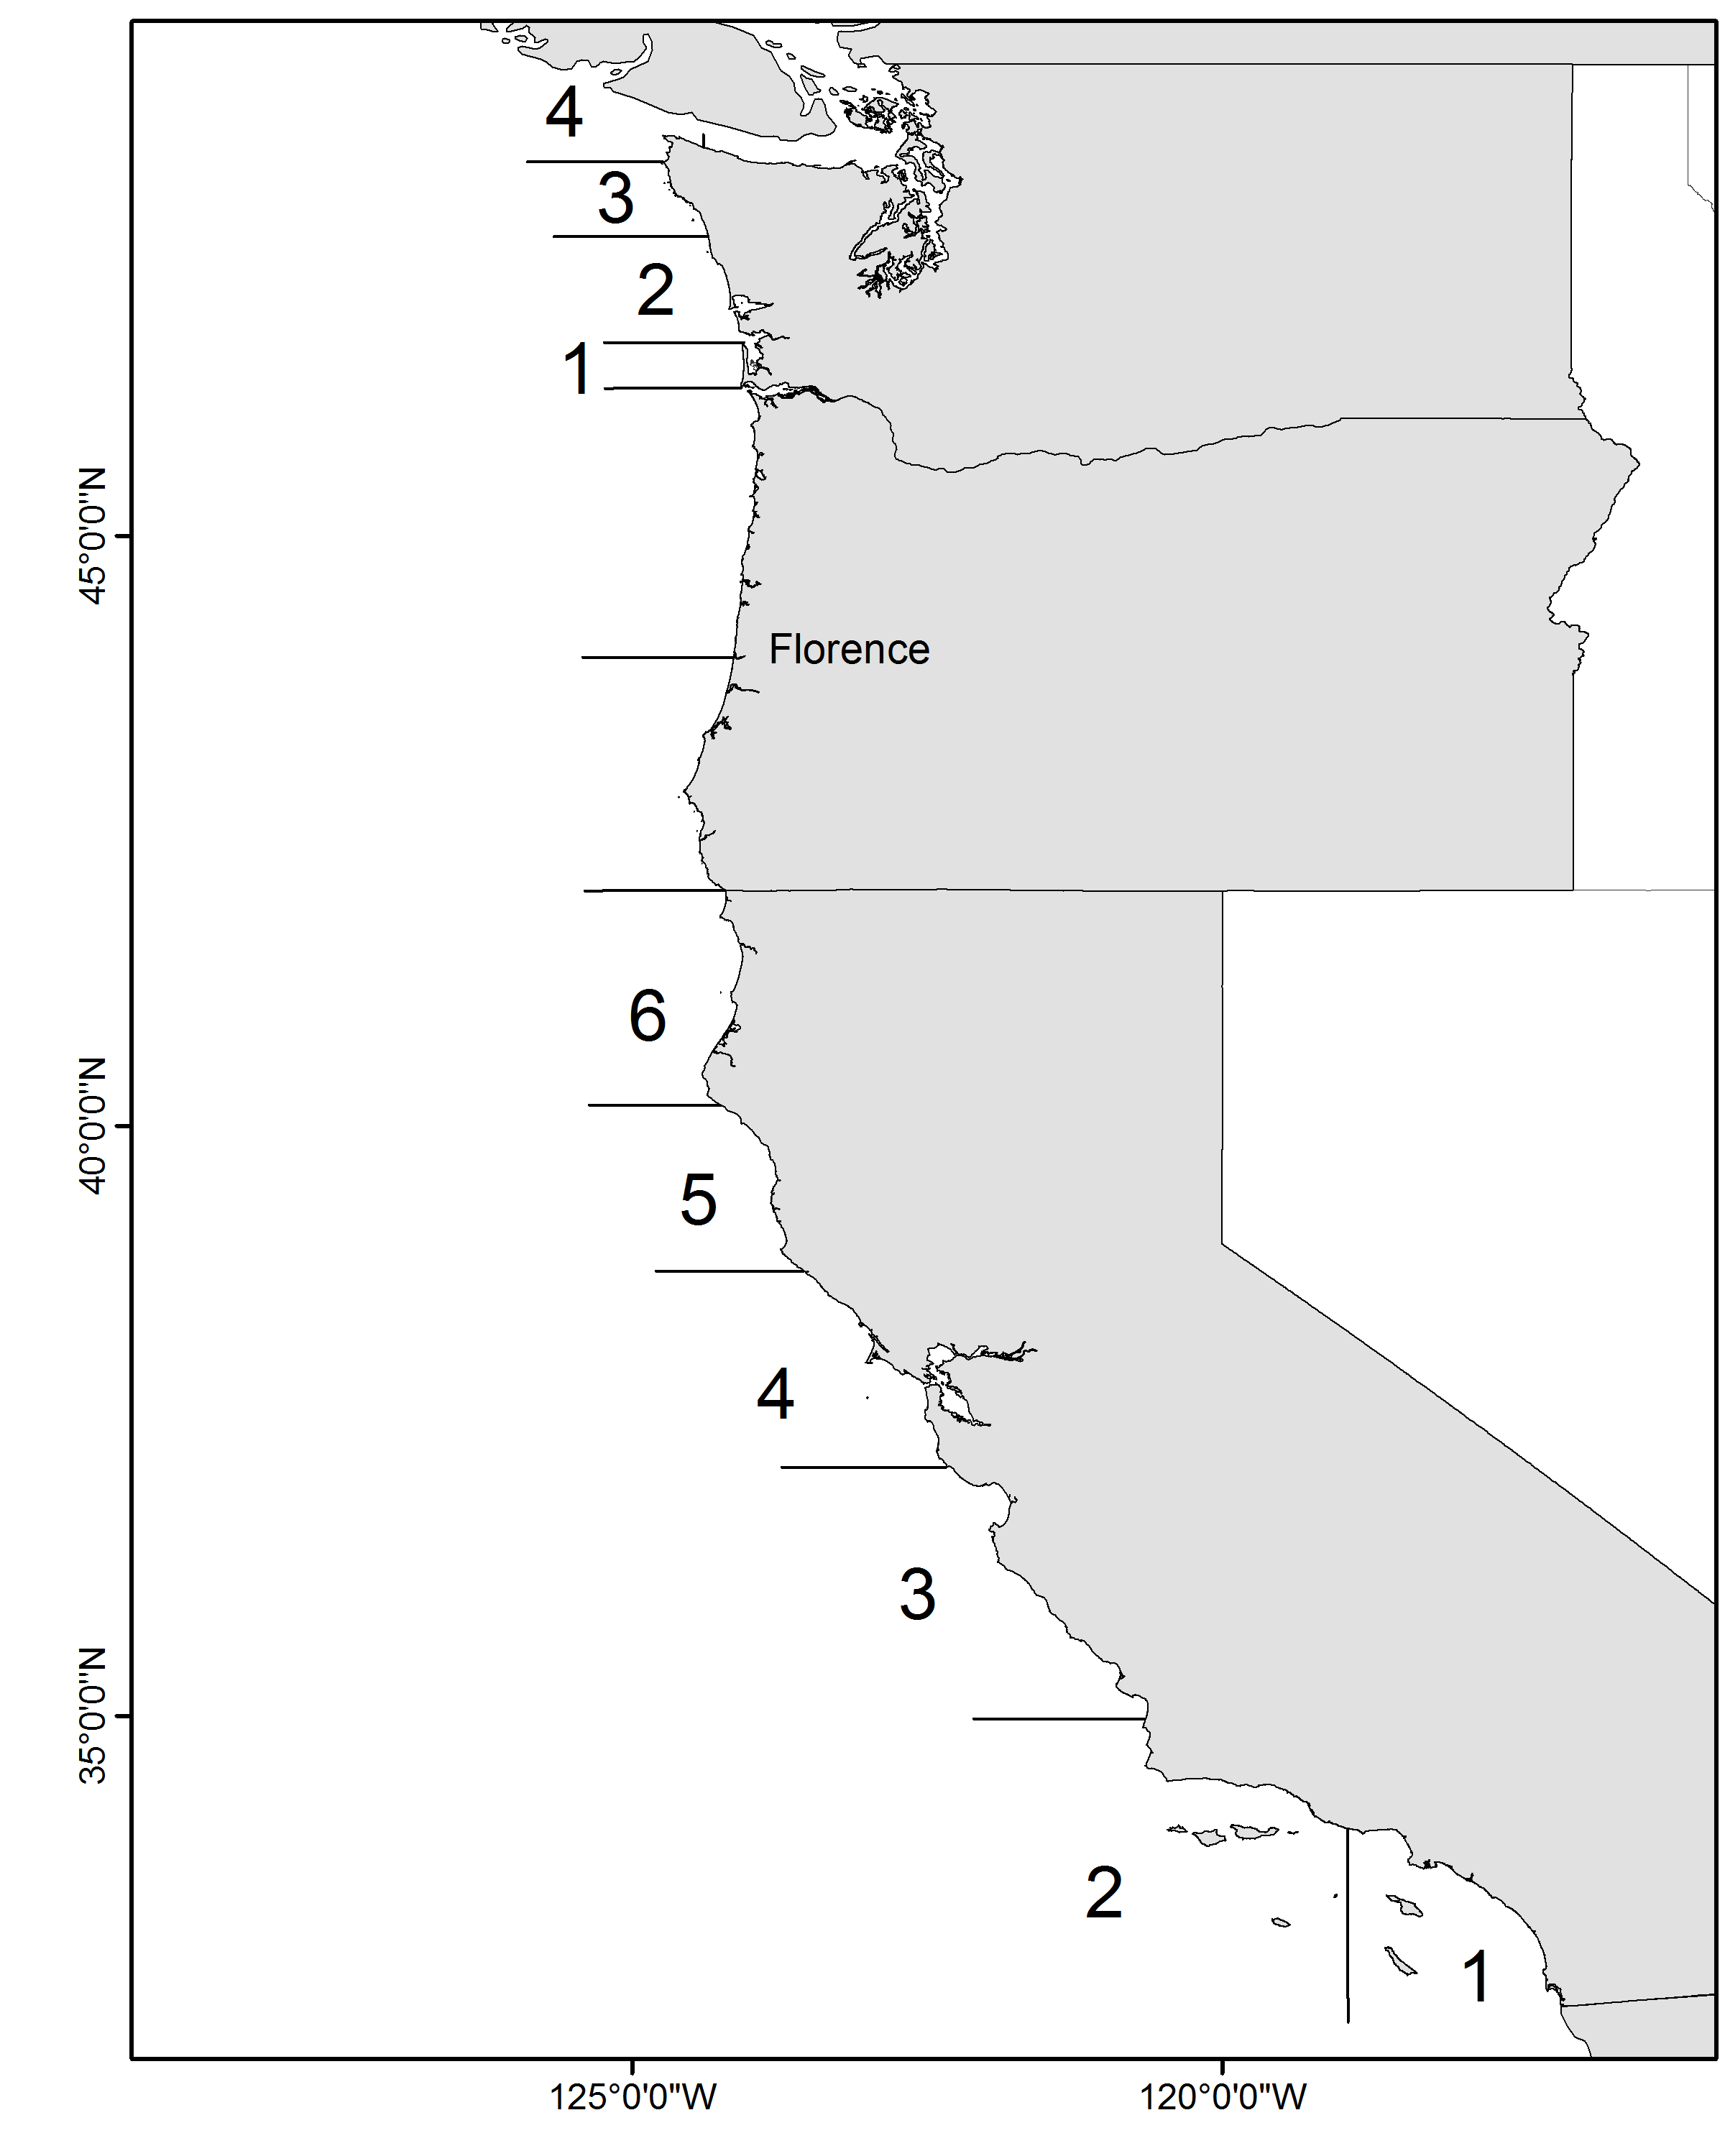
\includegraphics{Figures/boundary_map.png}
\caption{Map showing the state boundary lines for management of the
recreational fishing fleets. CRFS Districts 1-6 in California are
presented as well as the WDFW Recreational Management Areas in
Washington. Florence, OR is shown as a potential location of model
stratification. \label{fig:boundary_map}}
\end{figure}

\begin{figure}
\centering
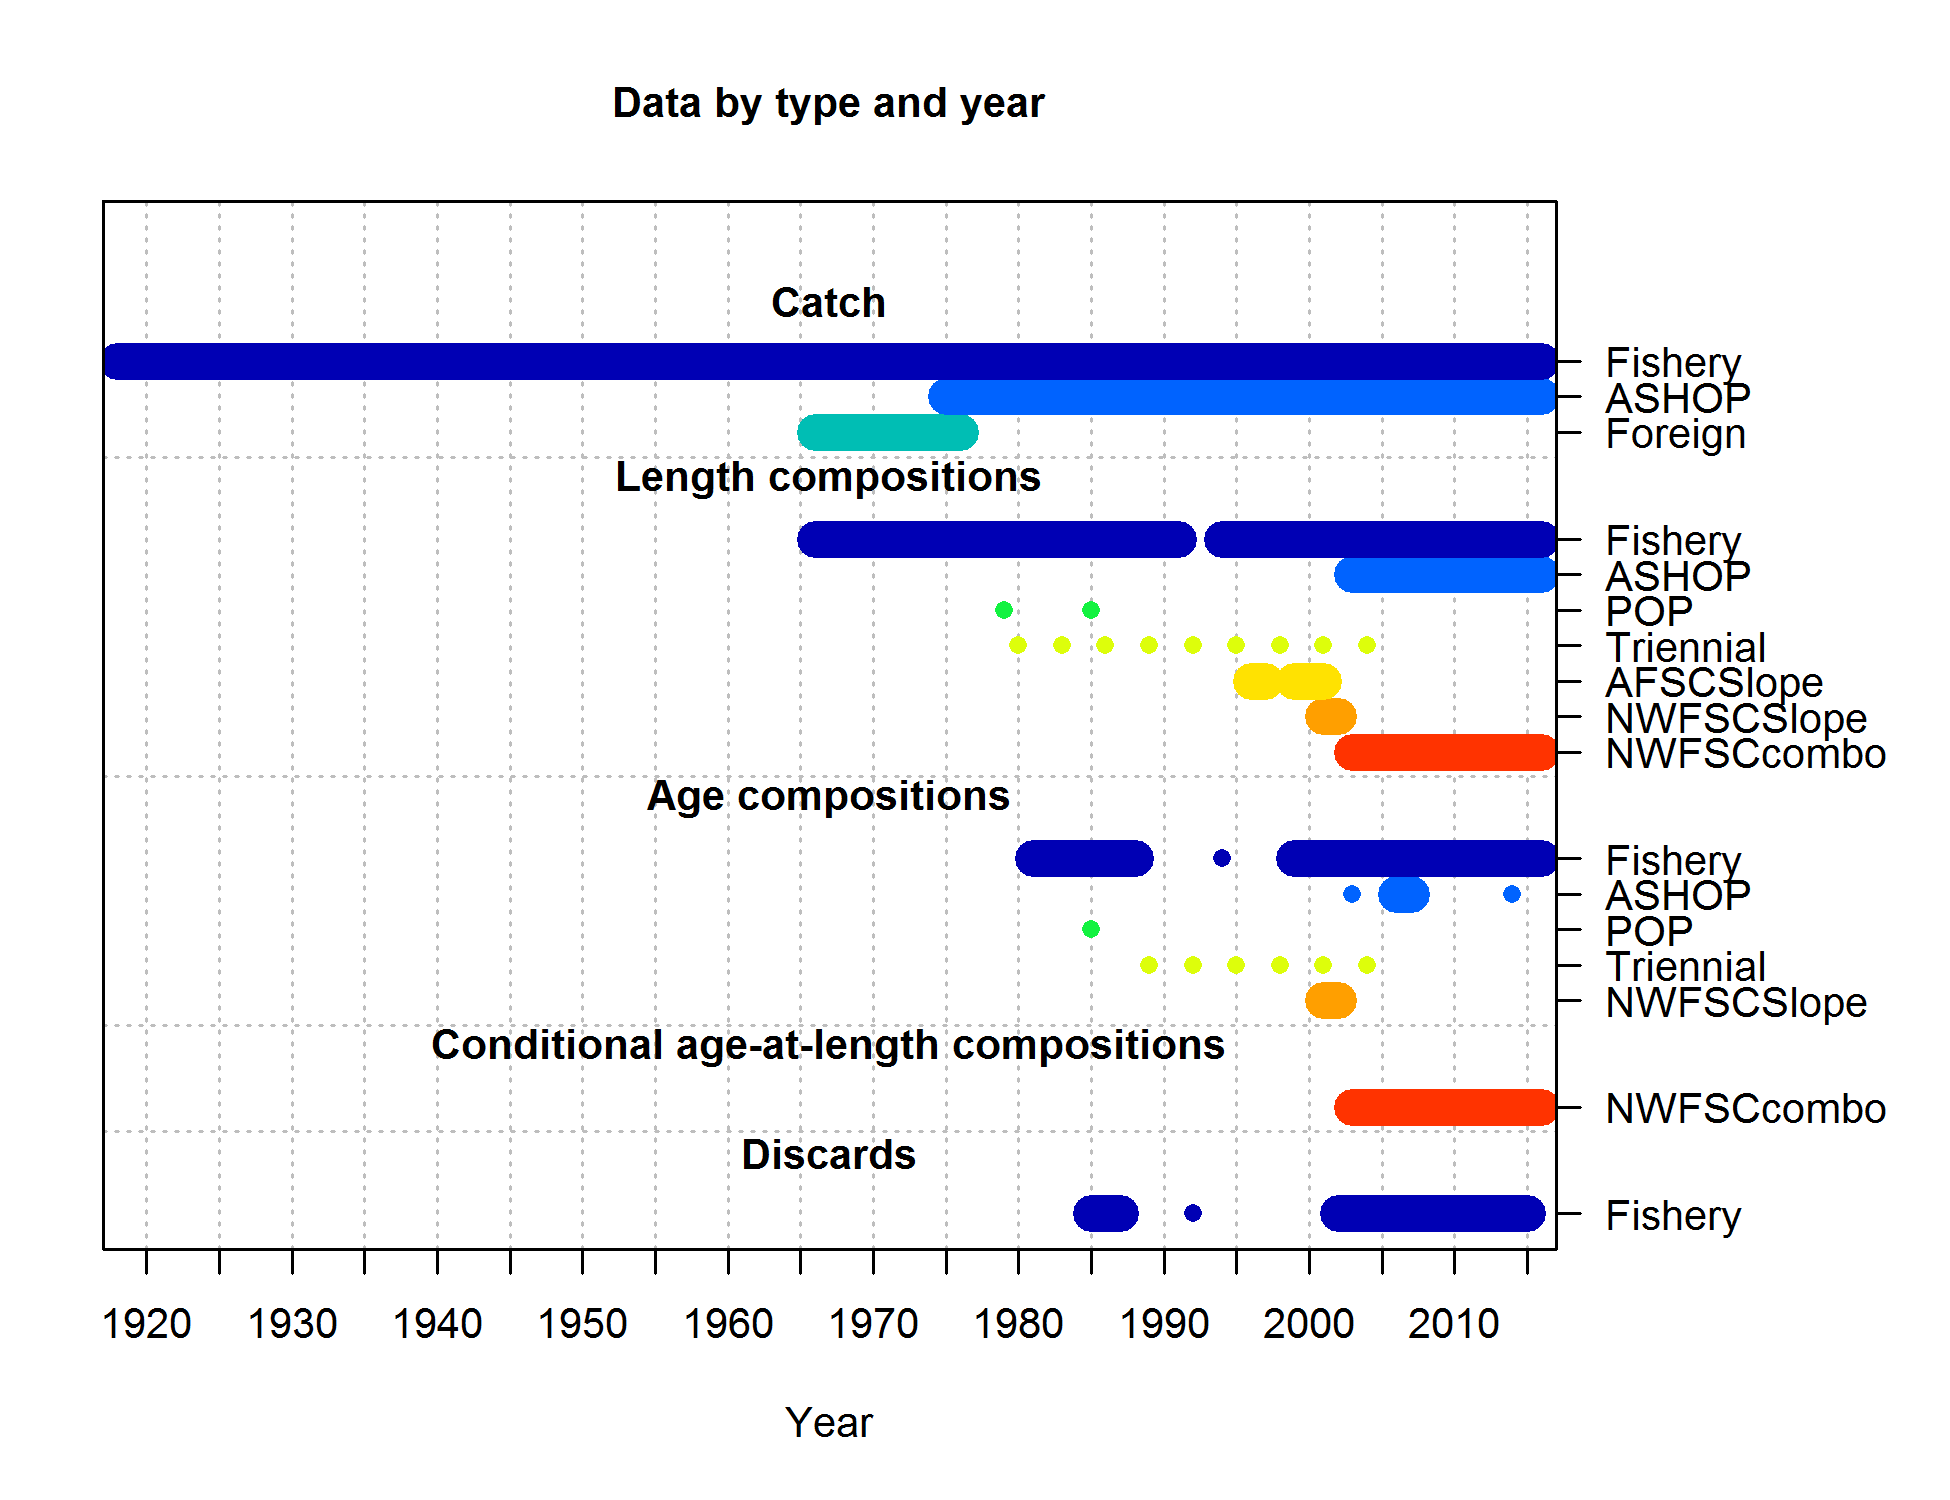
\includegraphics{r4ss/plots_mod1/data_plot.png}
\caption{Summary of data sources used in the Base model.
\label{fig:data_plot}}
\end{figure}

\FloatBarrier

\FloatBarrier

\begin{figure}
\centering
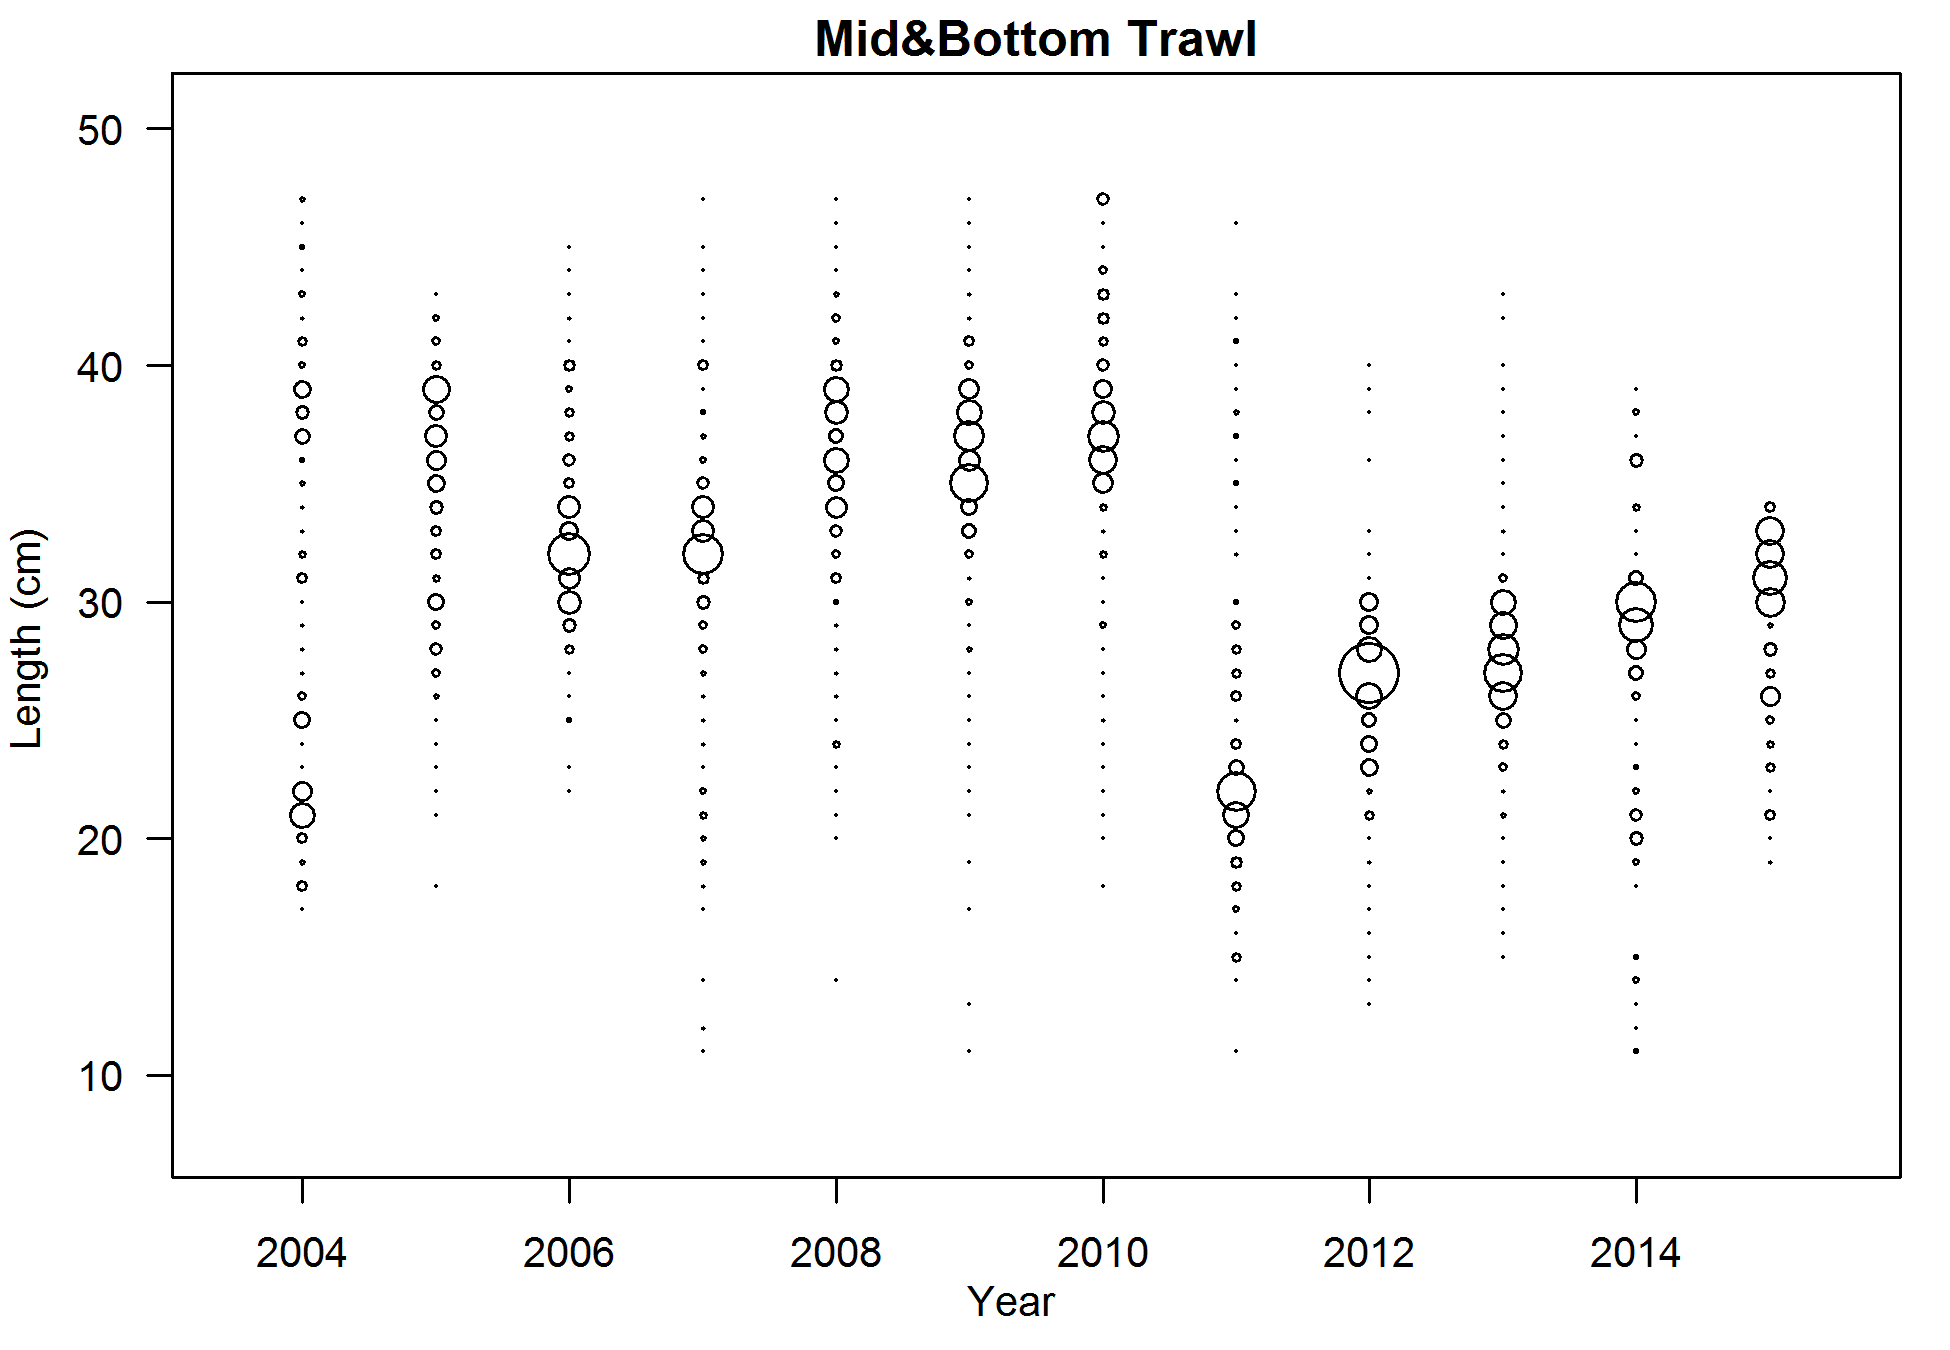
\includegraphics{Figures/discardLengthComps.png}
\caption{Discard length frequency distributions from the WCGOP for
Pacific ocean perch. \label{fig:WCGOP_discard}}
\end{figure}

\FloatBarrier

\FloatBarrier

\FloatBarrier

\FloatBarrier

\begin{figure}
\centering
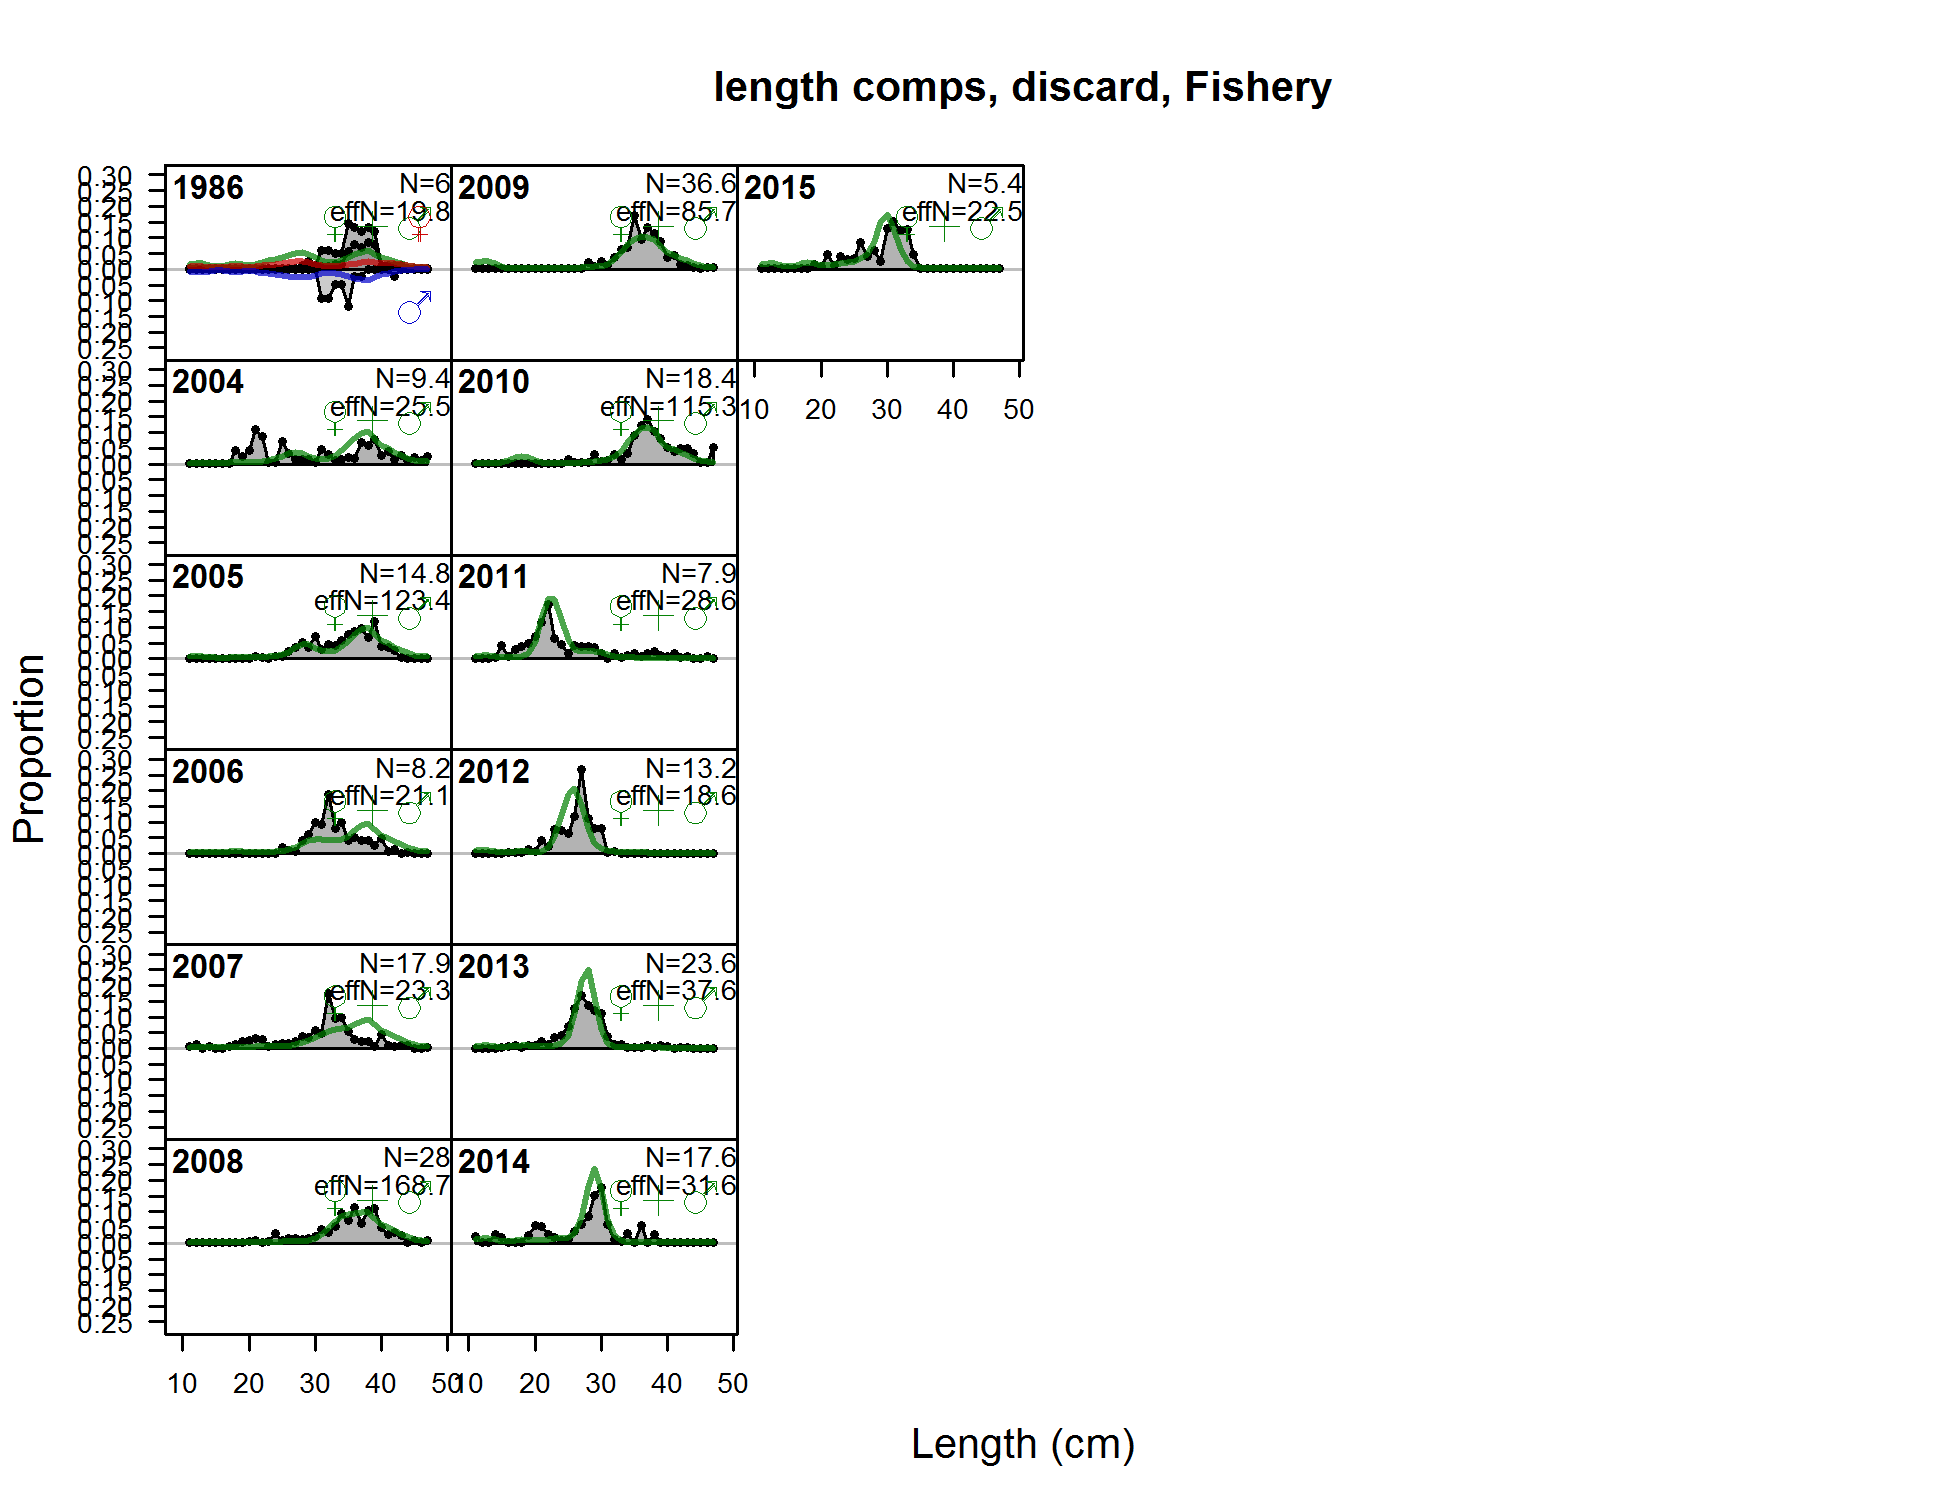
\includegraphics{./r4ss/plots_mod1/comp_lenfit_flt1mkt1.png}
\caption{length comps, discard, Fishery
\label{fig:mod1_1_comp_lenfit_flt1mkt1}}
\end{figure}

\begin{figure}
\centering
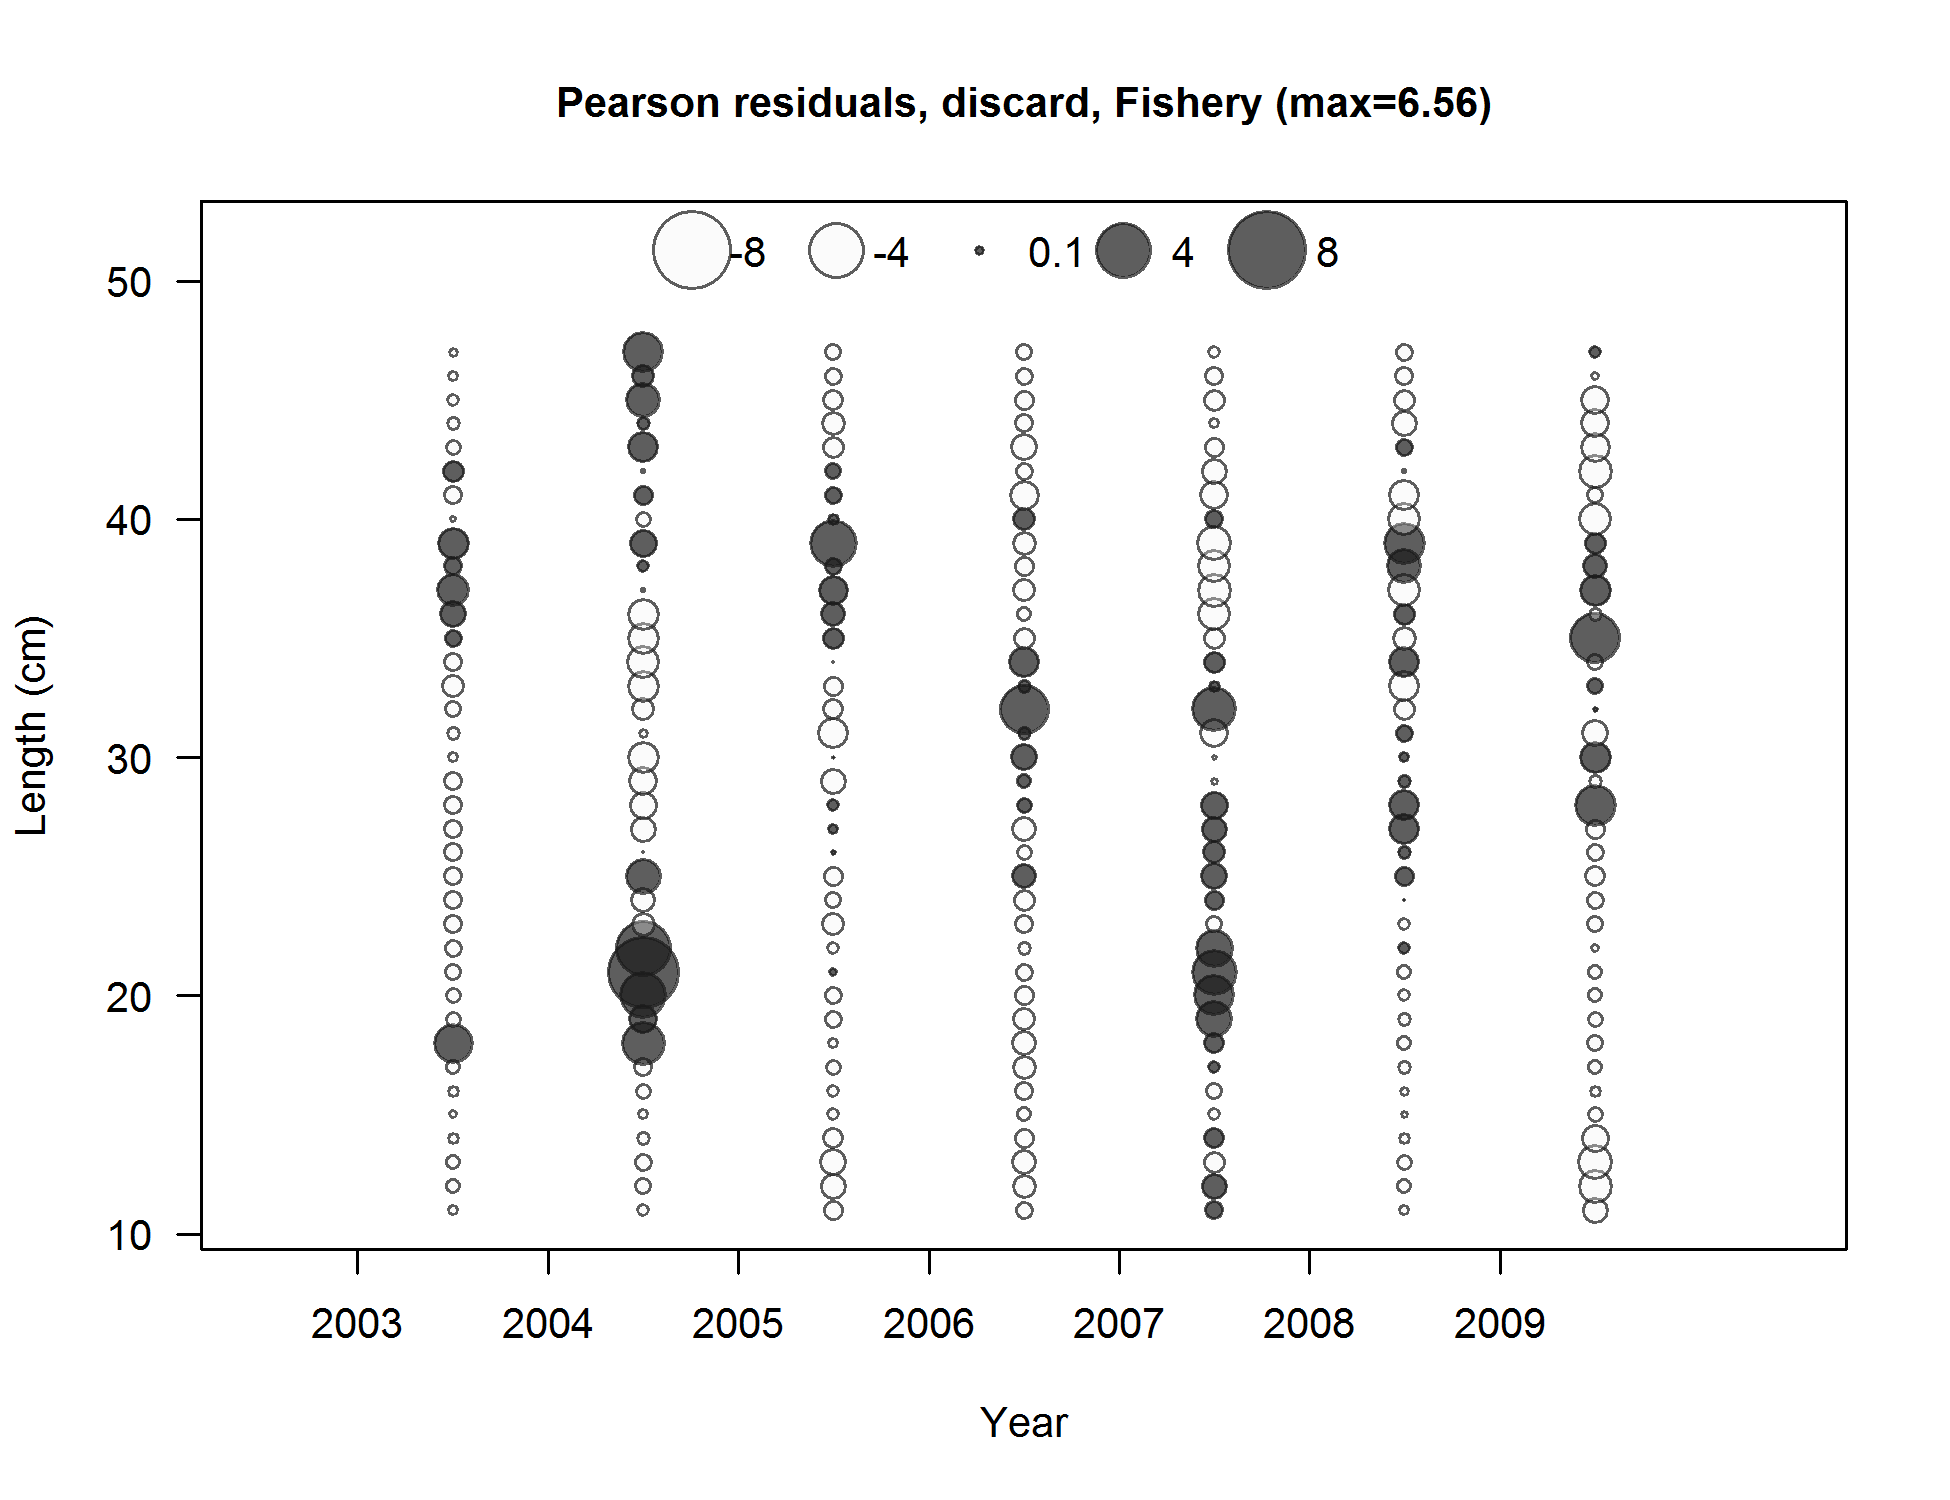
\includegraphics{./r4ss/plots_mod1/comp_lenfit_residsflt1mkt1.png}
\caption{Pearson residuals, discard, Fishery (max=4.71)\\
Closed bubbles are positive residuals (observed \textgreater{} expected)
and open bubbles are negative residuals (observed \textless{} expected).
\label{fig:mod1_2_comp_lenfit_residsflt1mkt1}}
\end{figure}

\begin{figure}
\centering
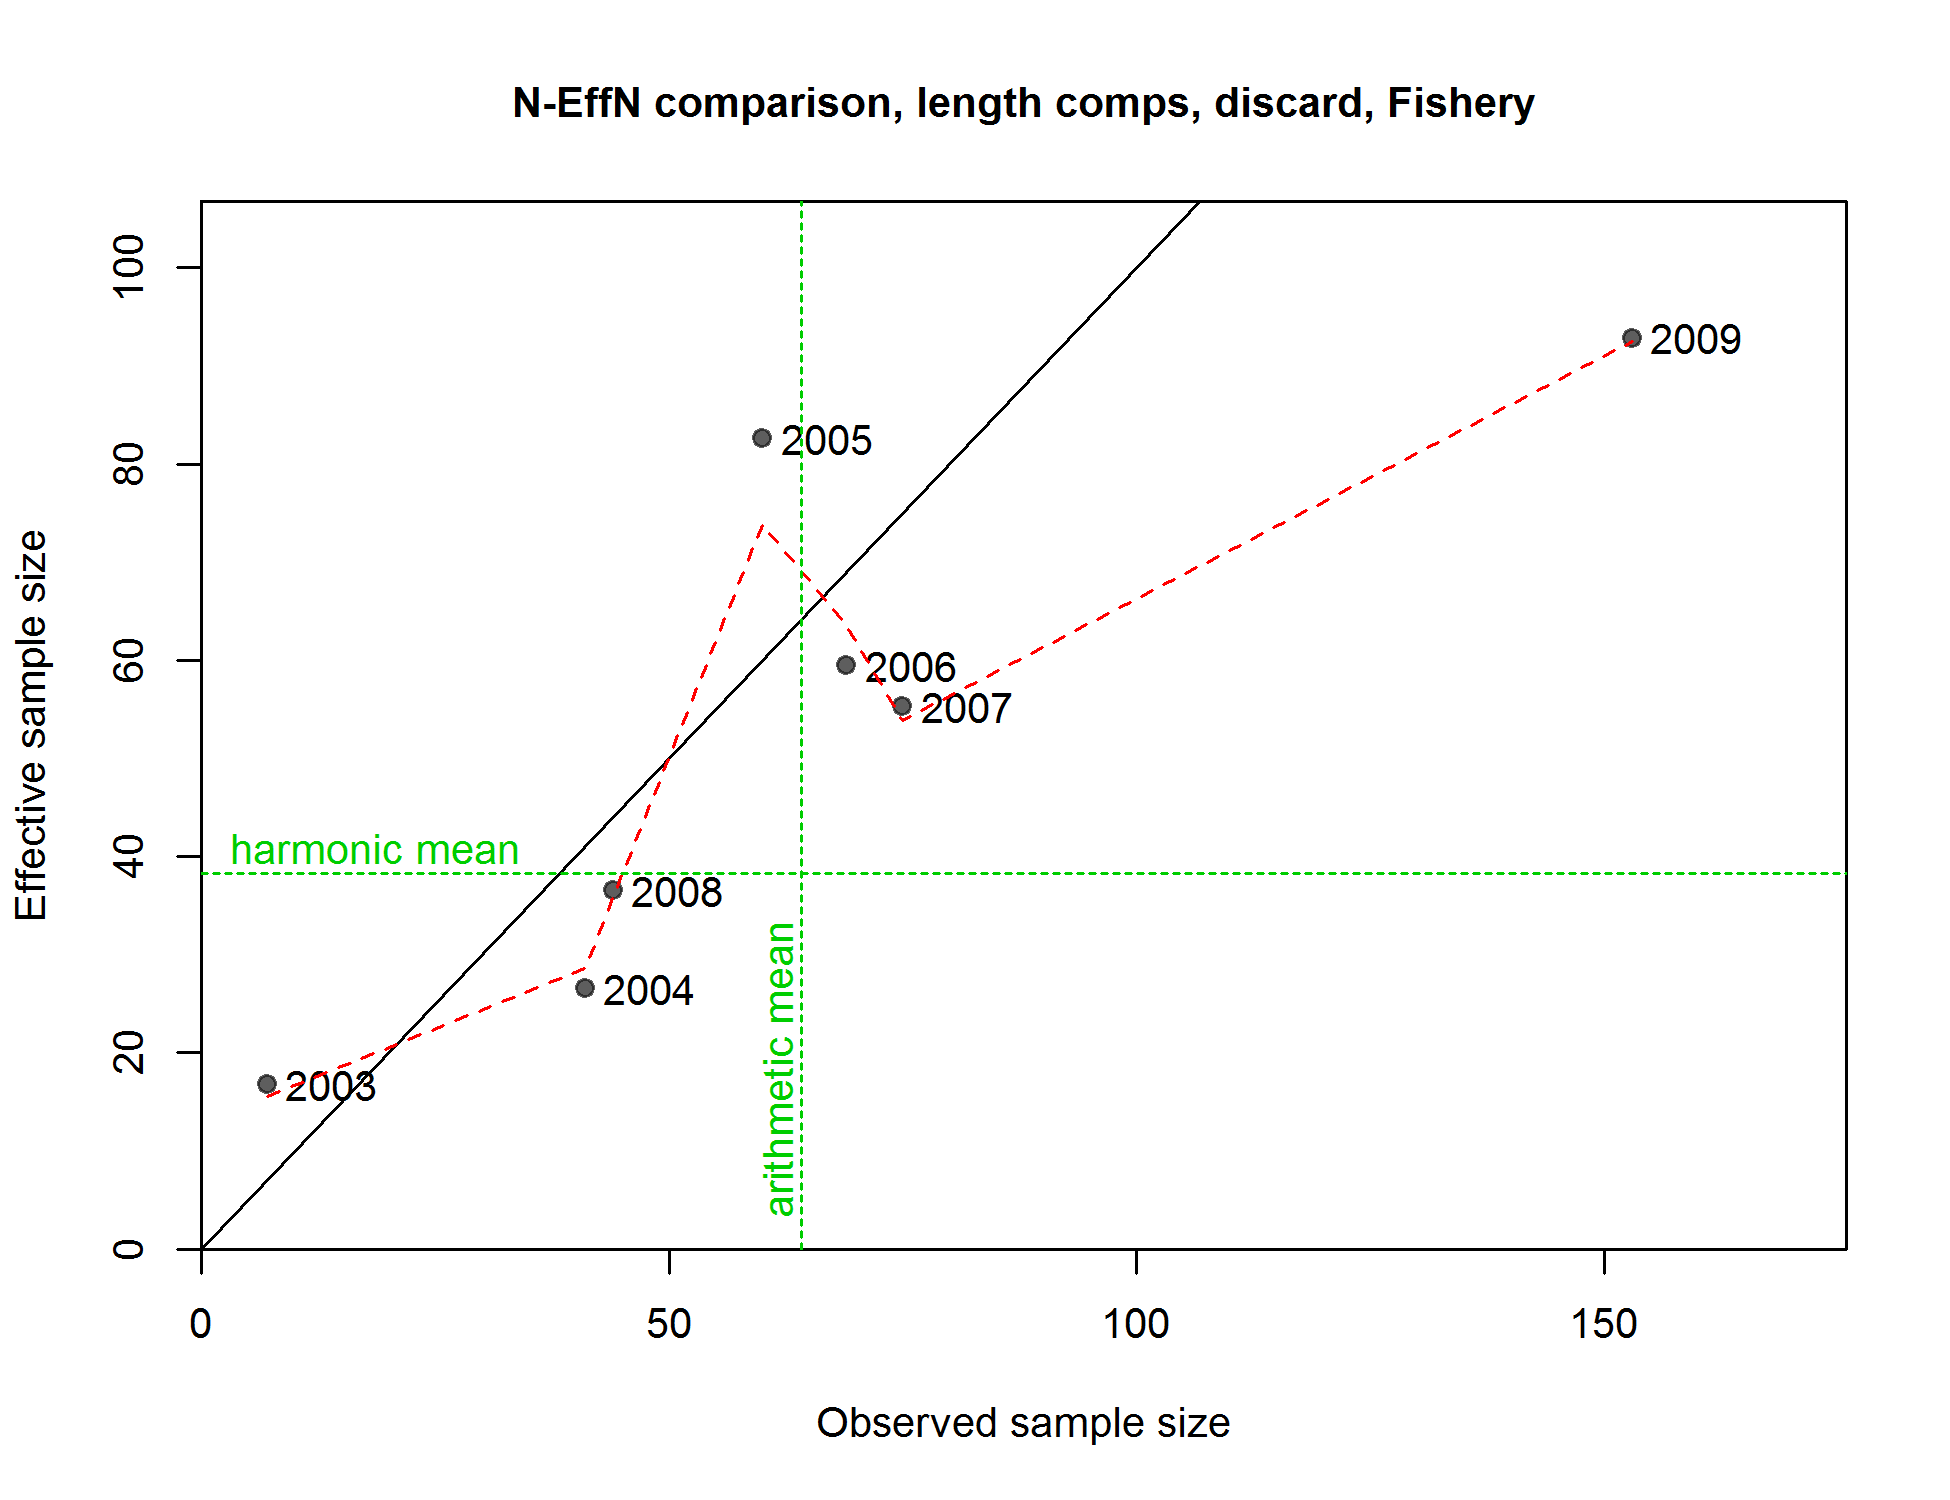
\includegraphics{./r4ss/plots_mod1/comp_lenfit_sampsize_flt1mkt1.png}
\caption{N\_EffN comparison, length comps, discard, Fishery
\label{fig:mod1_3_comp_lenfit_sampsize_flt1mkt1}}
\end{figure}

\begin{figure}
\centering
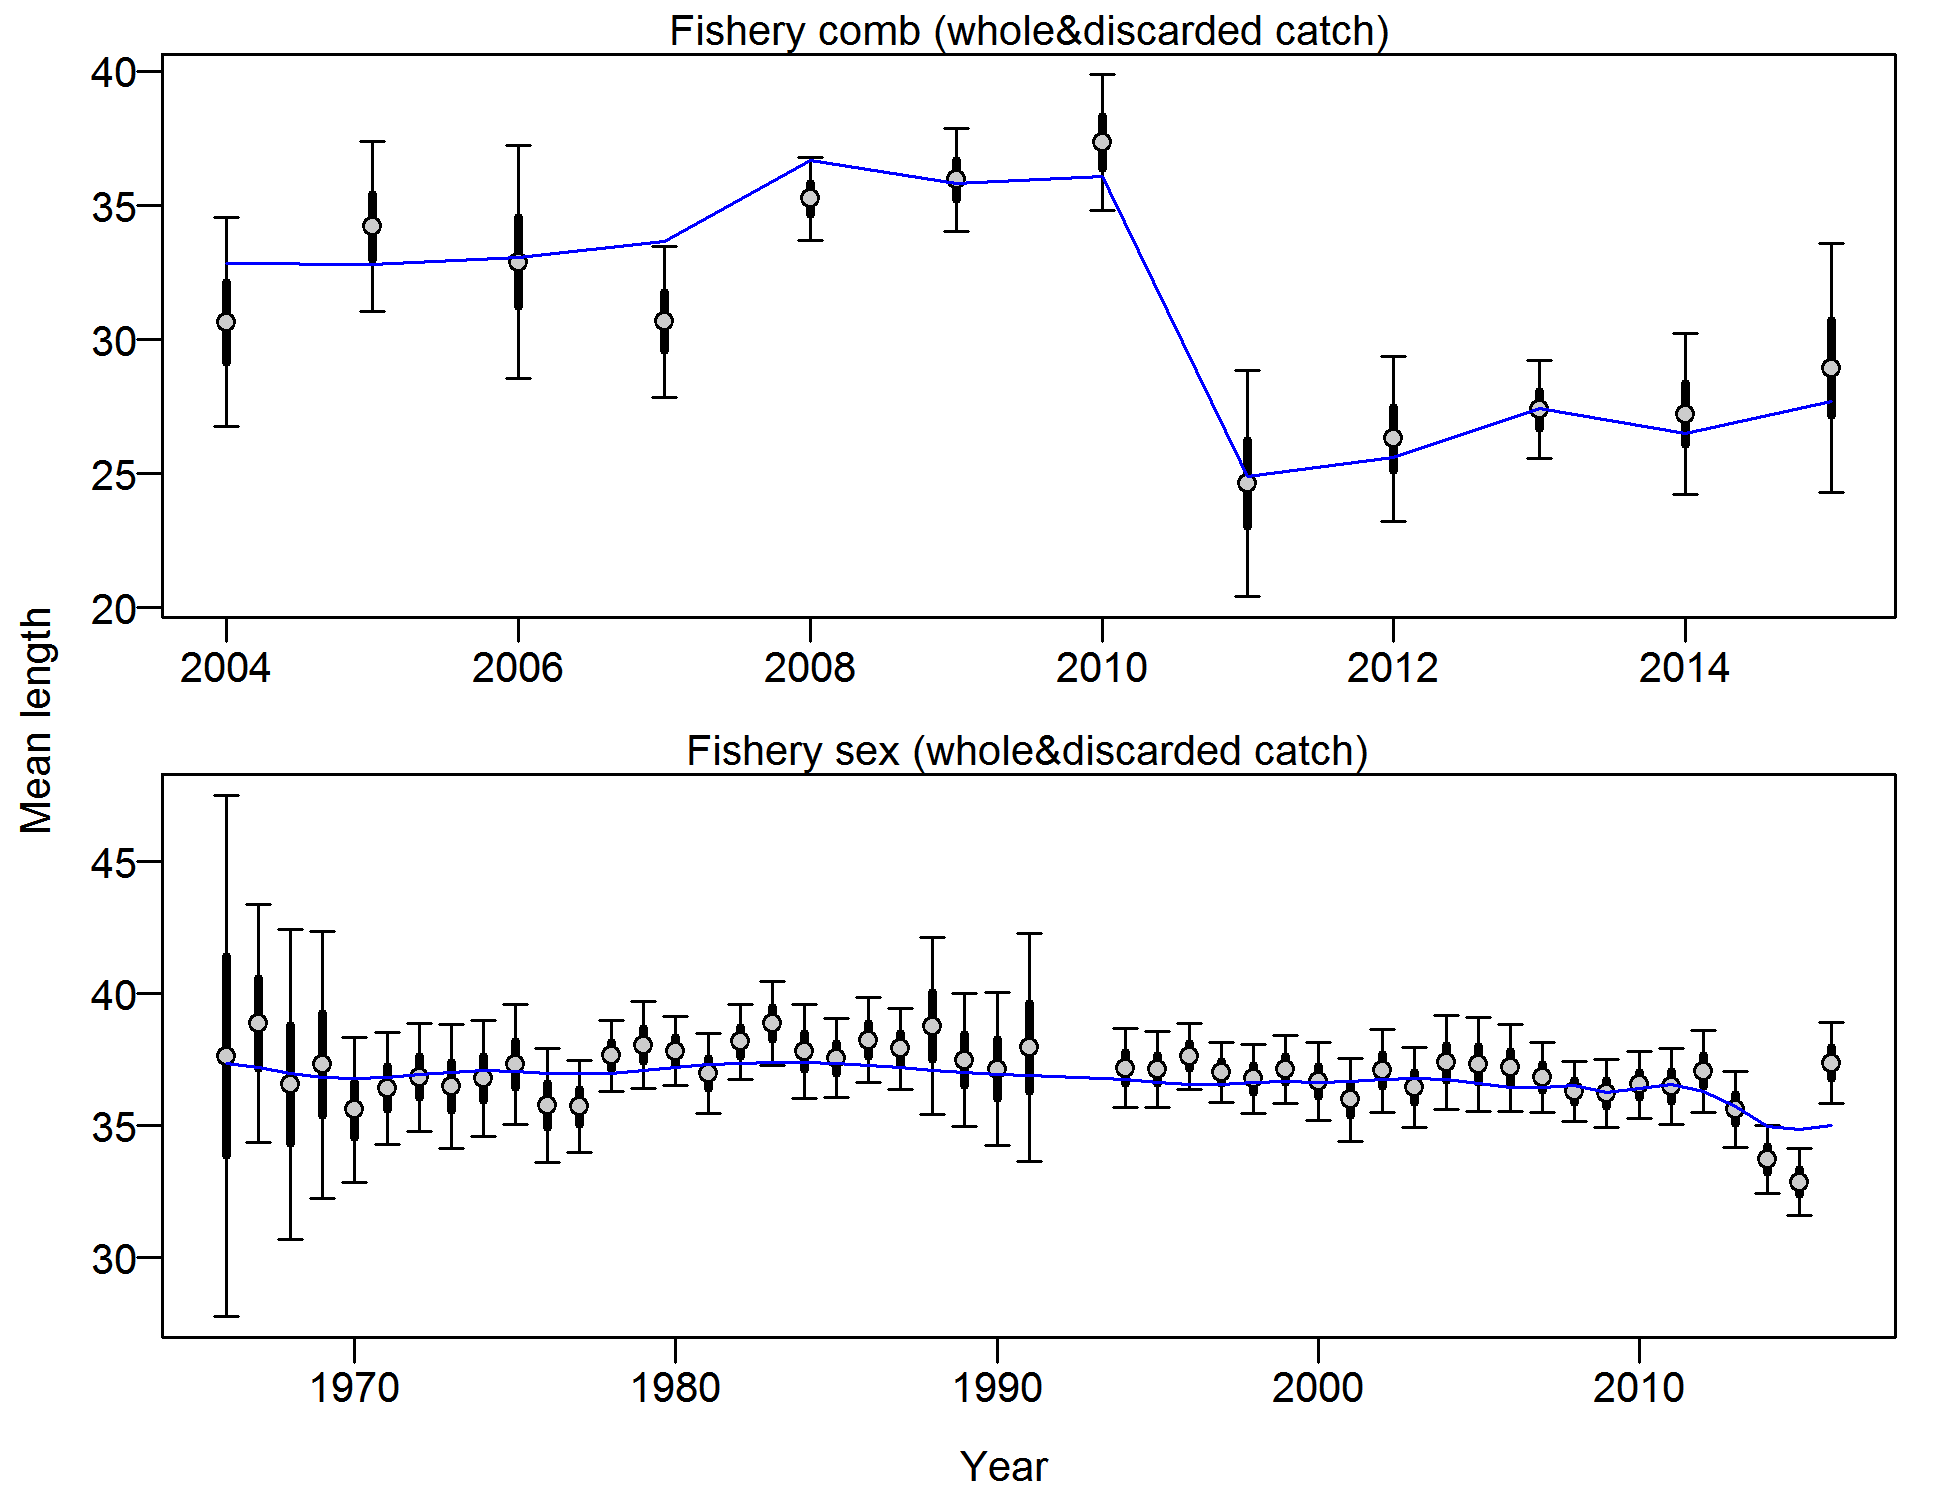
\includegraphics{./r4ss/plots_mod1/comp_lenfit_data_weighting_TA1.8_Fishery.png}
\caption{Francis data weighting method TA1.8 Fishery Suggested sample
size adjustment (with 95\% interval) for len data from Fishery: 0.8226
(0.5299\_1.5611)
\label{fig:mod1_4_comp_lenfit_data_weighting_TA1.8_Fishery}}
\end{figure}

\begin{figure}
\centering
\includegraphics{./r4ss/plots_mod1/comp_lenfit_flt1mkt2_page1.png}
\caption{length comps, retained, Fishery (plot 1 of 2)
\label{fig:mod1_5_comp_lenfit_flt1mkt2_page1}}
\end{figure}

\includegraphics{./r4ss/plots_mod1/comp_lenfit_flt1mkt2_page2.png}

\begin{center} 

        Figure continued from previous page 

        \end{center}

\includegraphics{./r4ss/plots_mod1/comp_lenfit_residsflt1mkt2_page2.png}

\begin{center} 

        Figure continued from previous page 

        \end{center}

\begin{figure}
\centering
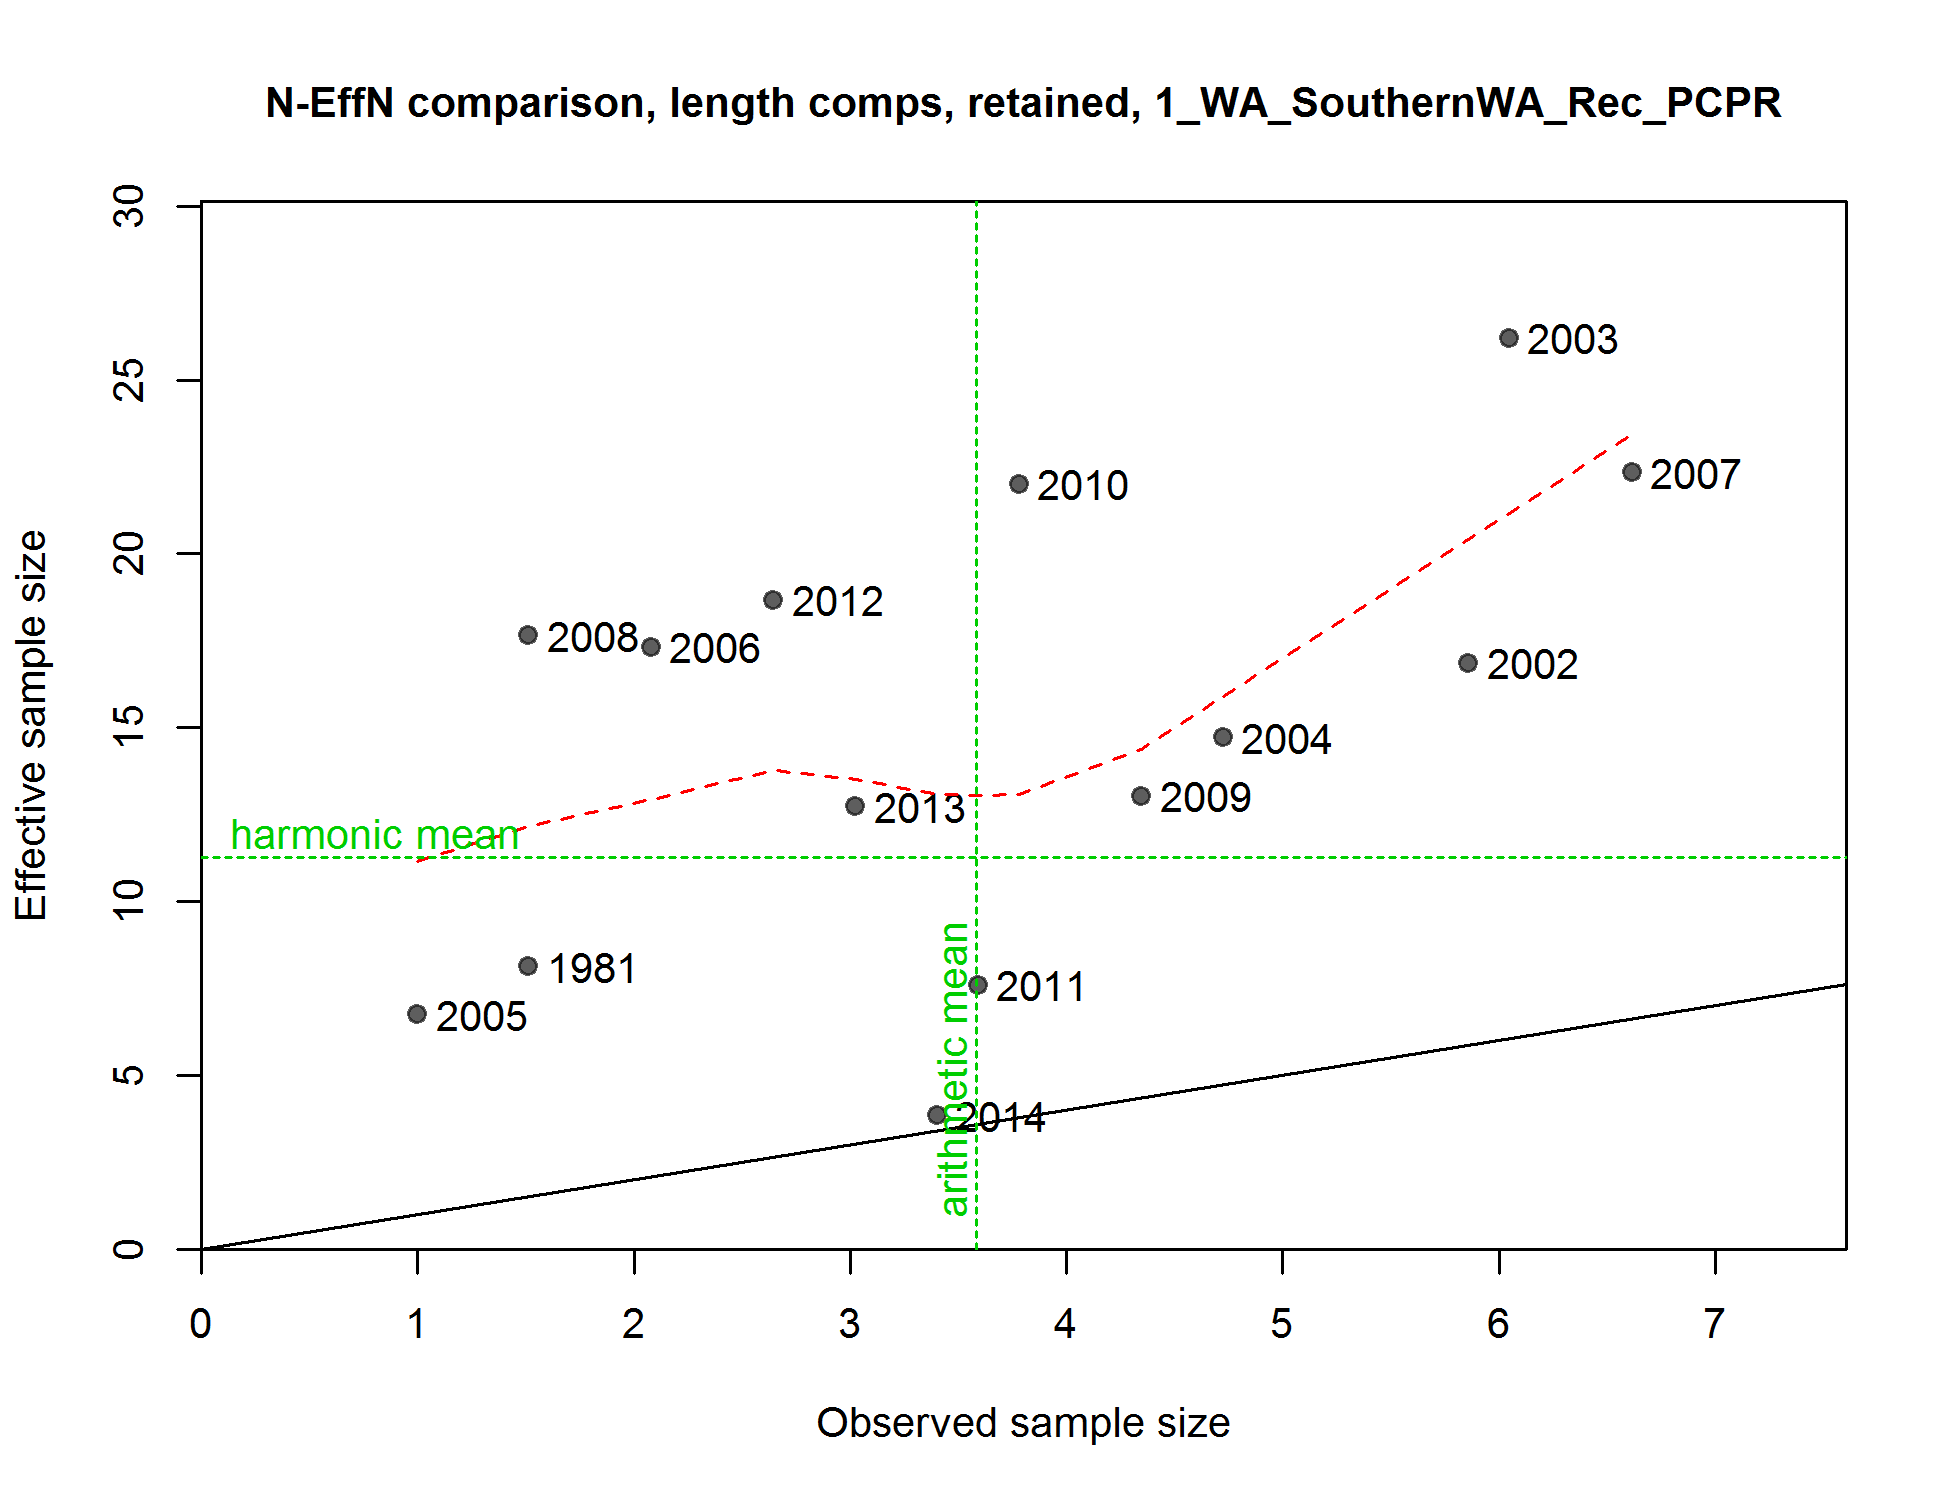
\includegraphics{./r4ss/plots_mod1/comp_lenfit_sampsize_flt1mkt2.png}
\caption{N\_EffN comparison, length comps, retained, Fishery
\label{fig:mod1_8_comp_lenfit_sampsize_flt1mkt2}}
\end{figure}

\begin{figure}
\centering
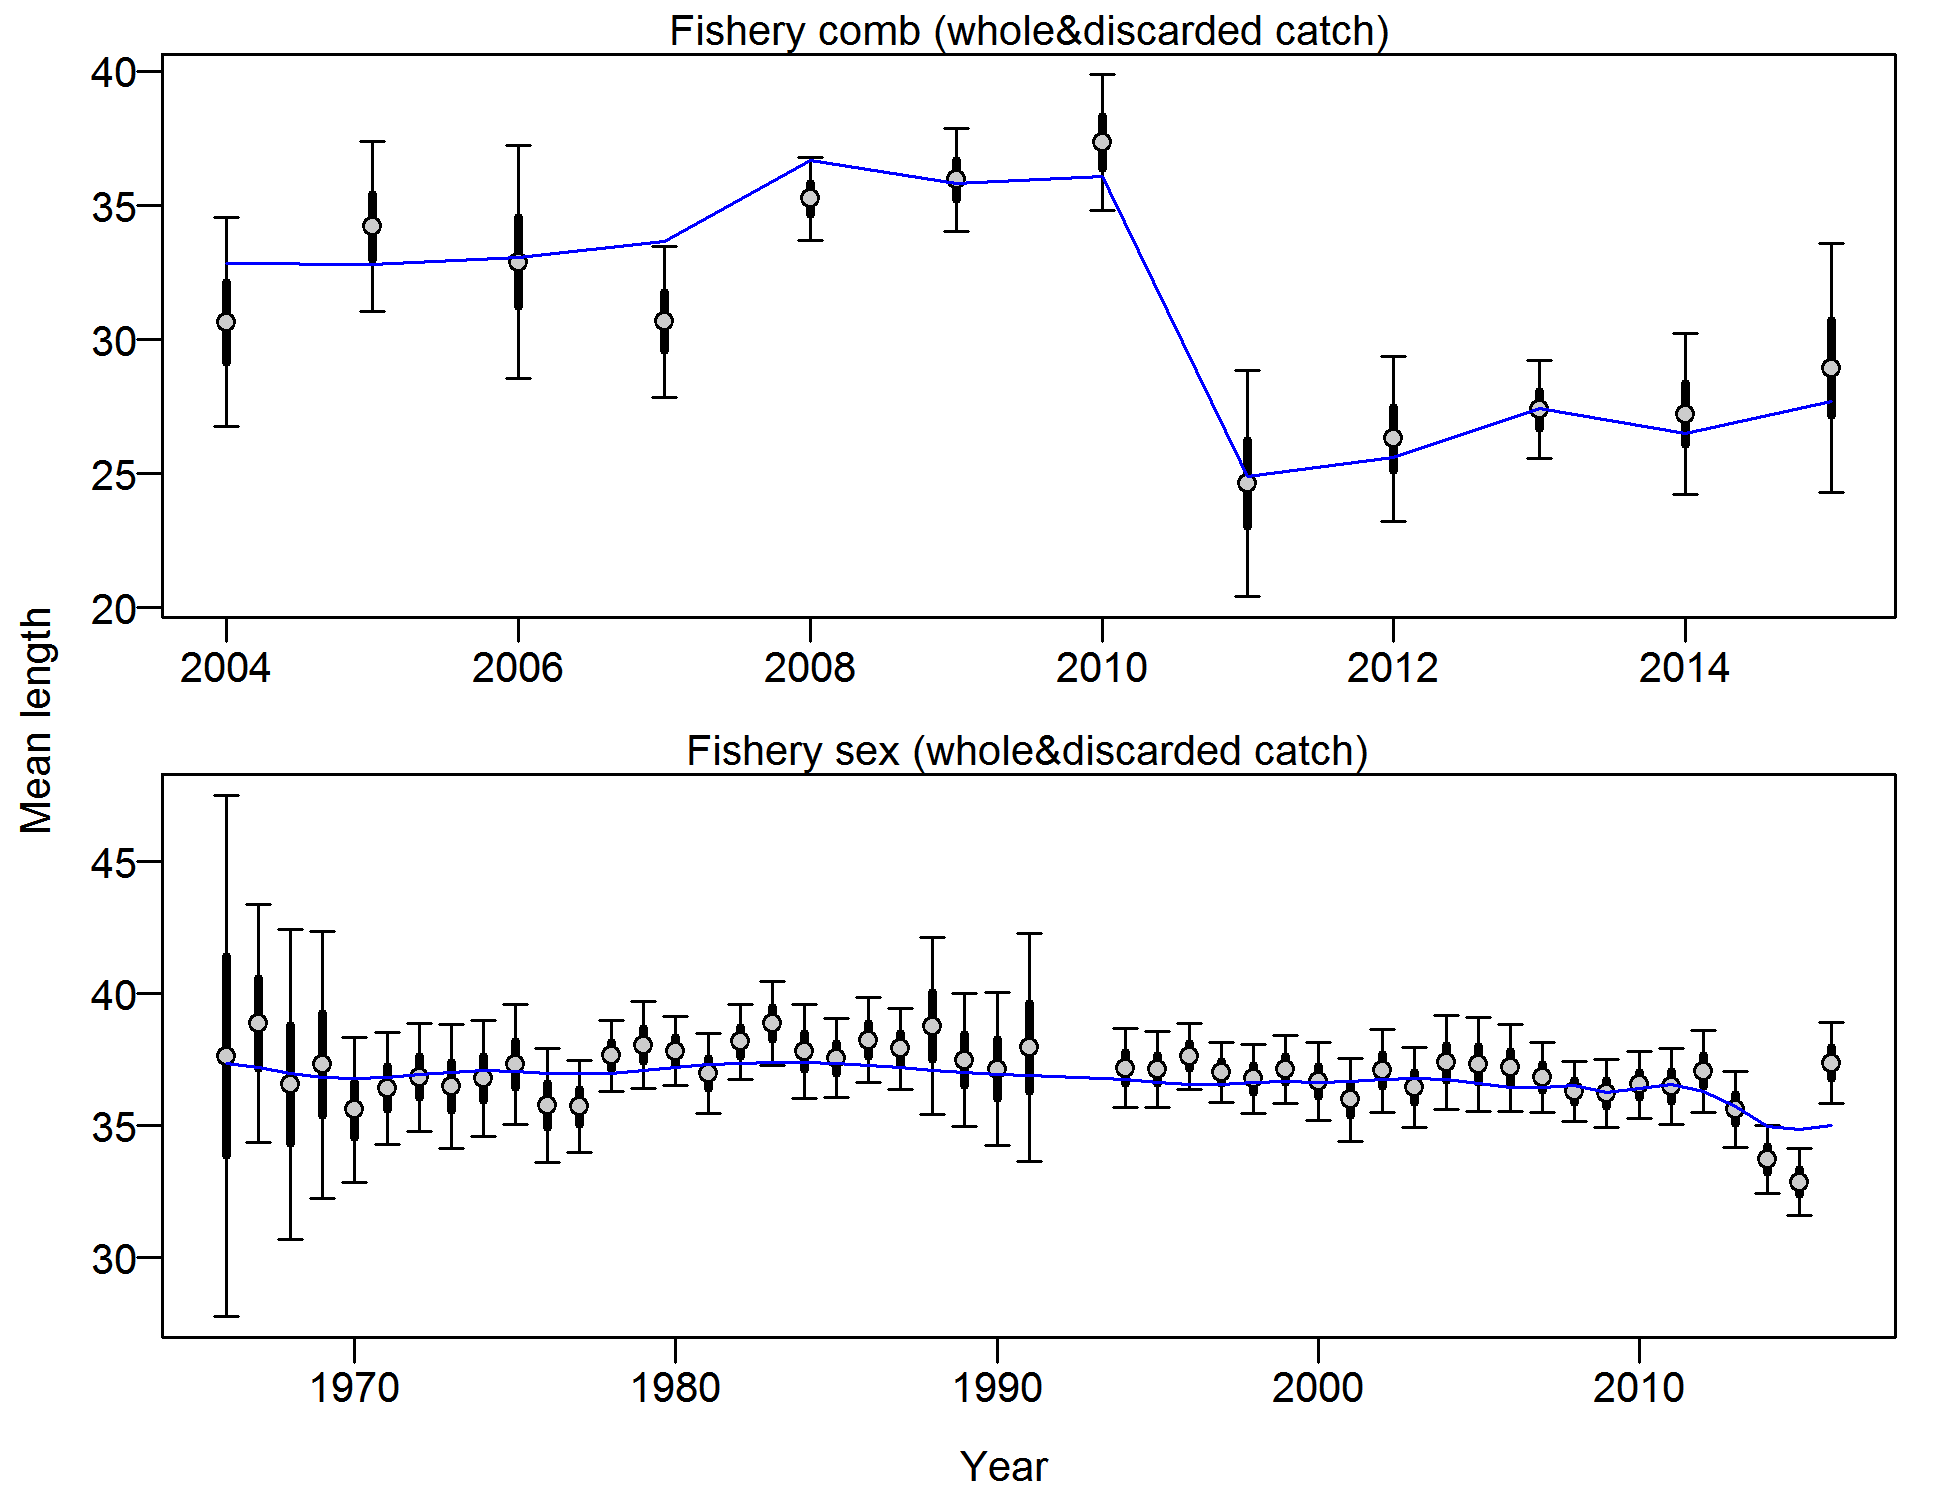
\includegraphics{./r4ss/plots_mod1/comp_lenfit_data_weighting_TA1.8_Fishery.png}
\caption{Francis data weighting method TA1.8 Fishery Suggested sample
size adjustment (with 95\% interval) for len data from Fishery: 0.8226
(0.5458\_1.505)
\label{fig:mod1_9_comp_lenfit_data_weighting_TA1.8_Fishery}}
\end{figure}

\begin{figure}
\centering
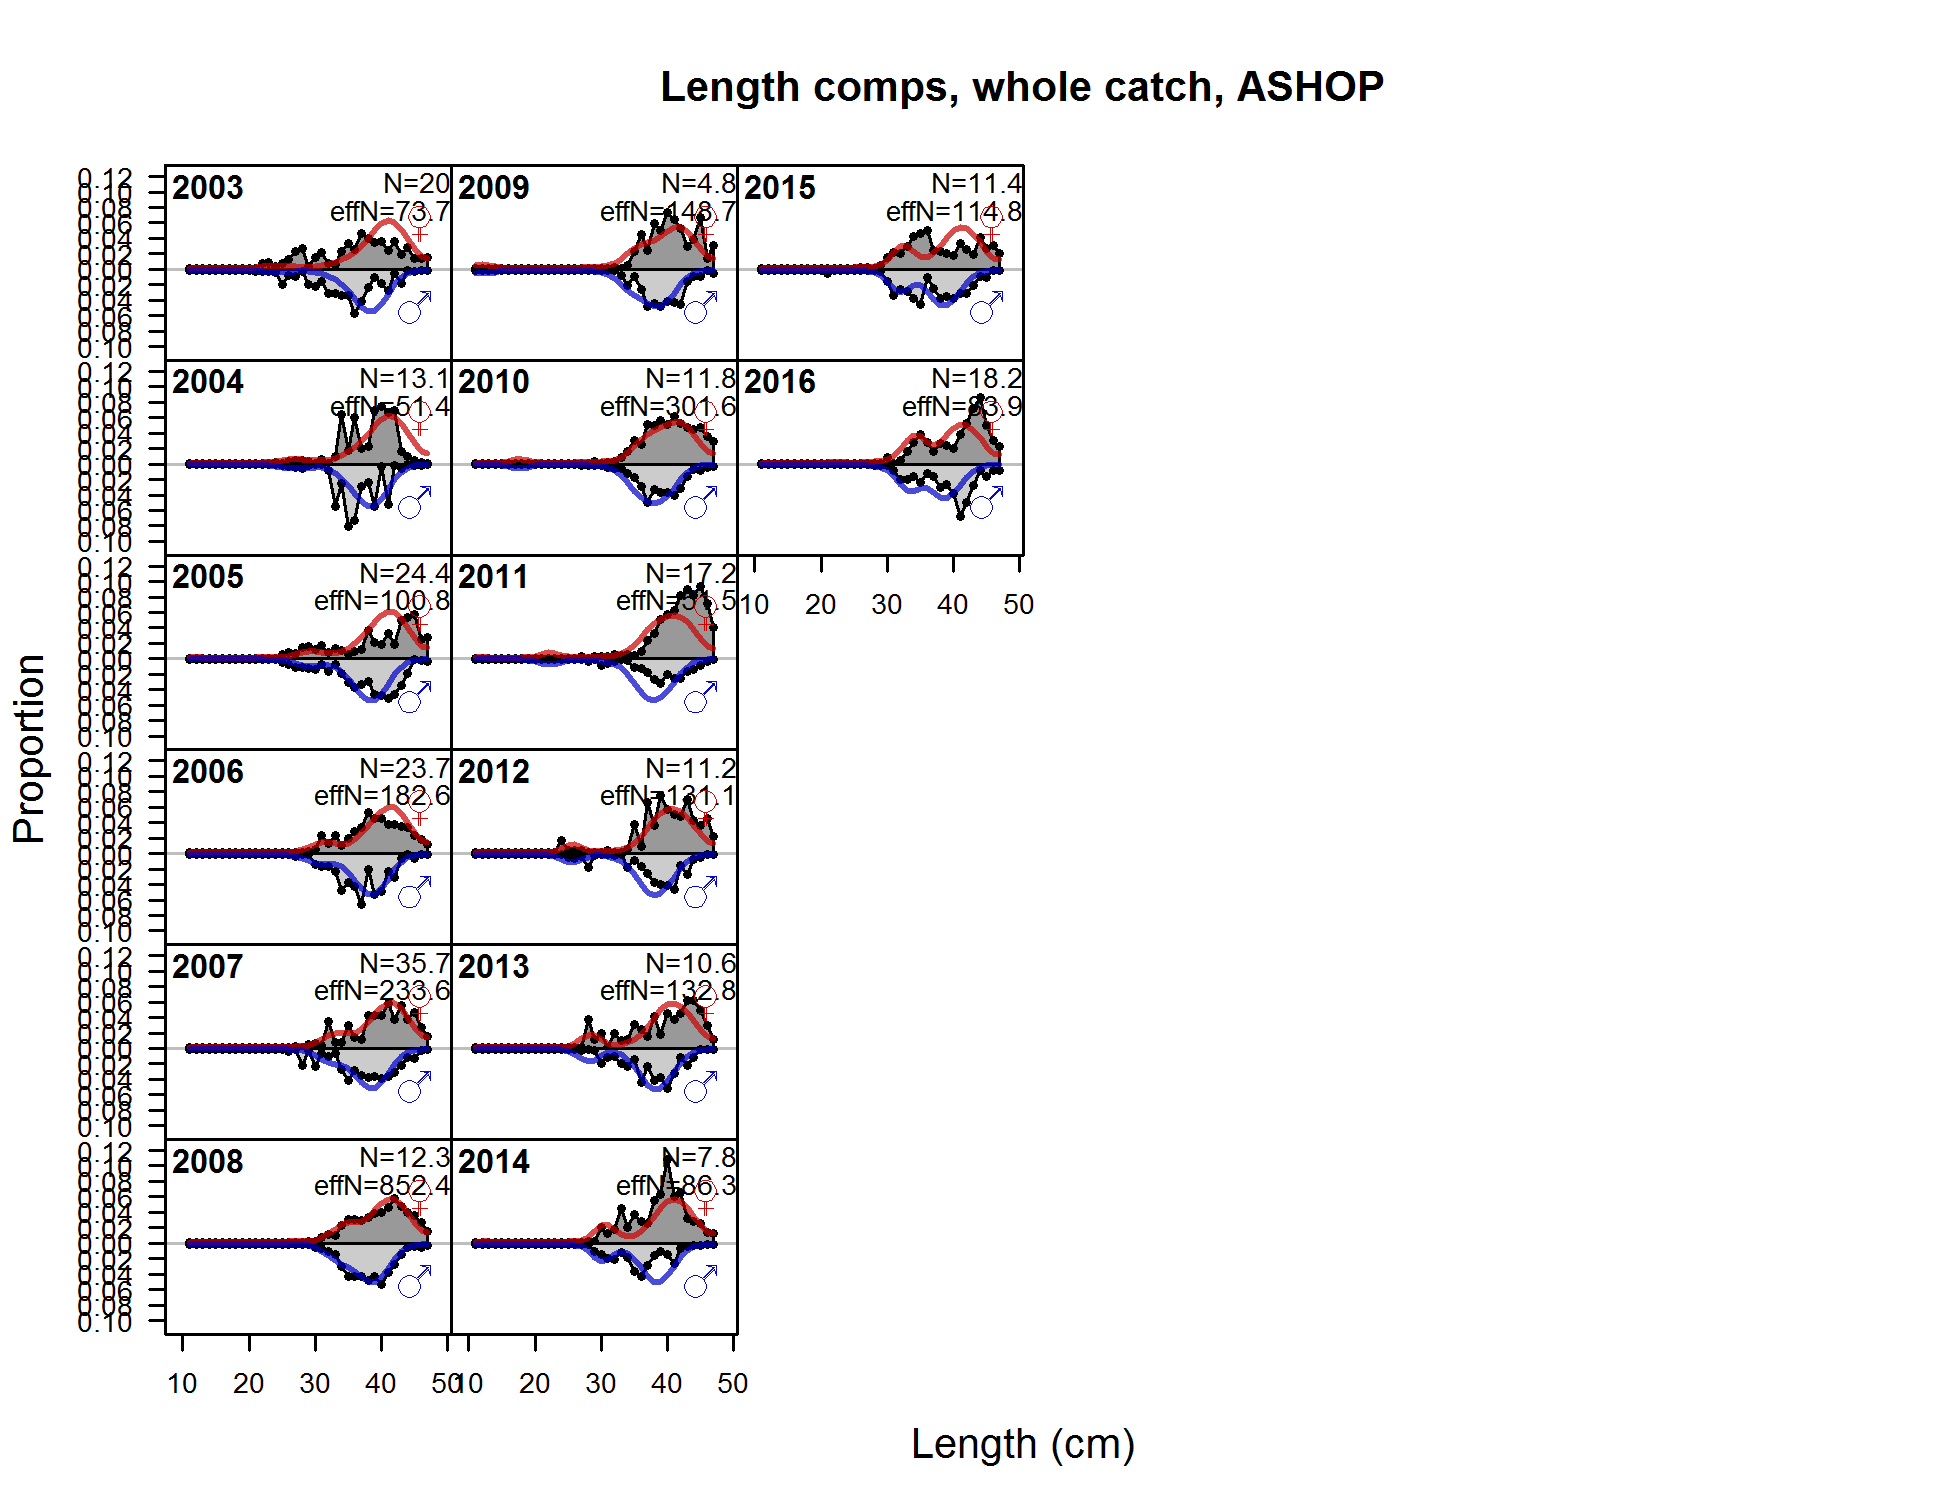
\includegraphics{./r4ss/plots_mod1/comp_lenfit_flt2mkt0.png}
\caption{length comps, whole catch, ASHOP
\label{fig:mod1_10_comp_lenfit_flt2mkt0}}
\end{figure}

\FloatBarrier

\begin{figure}
\centering
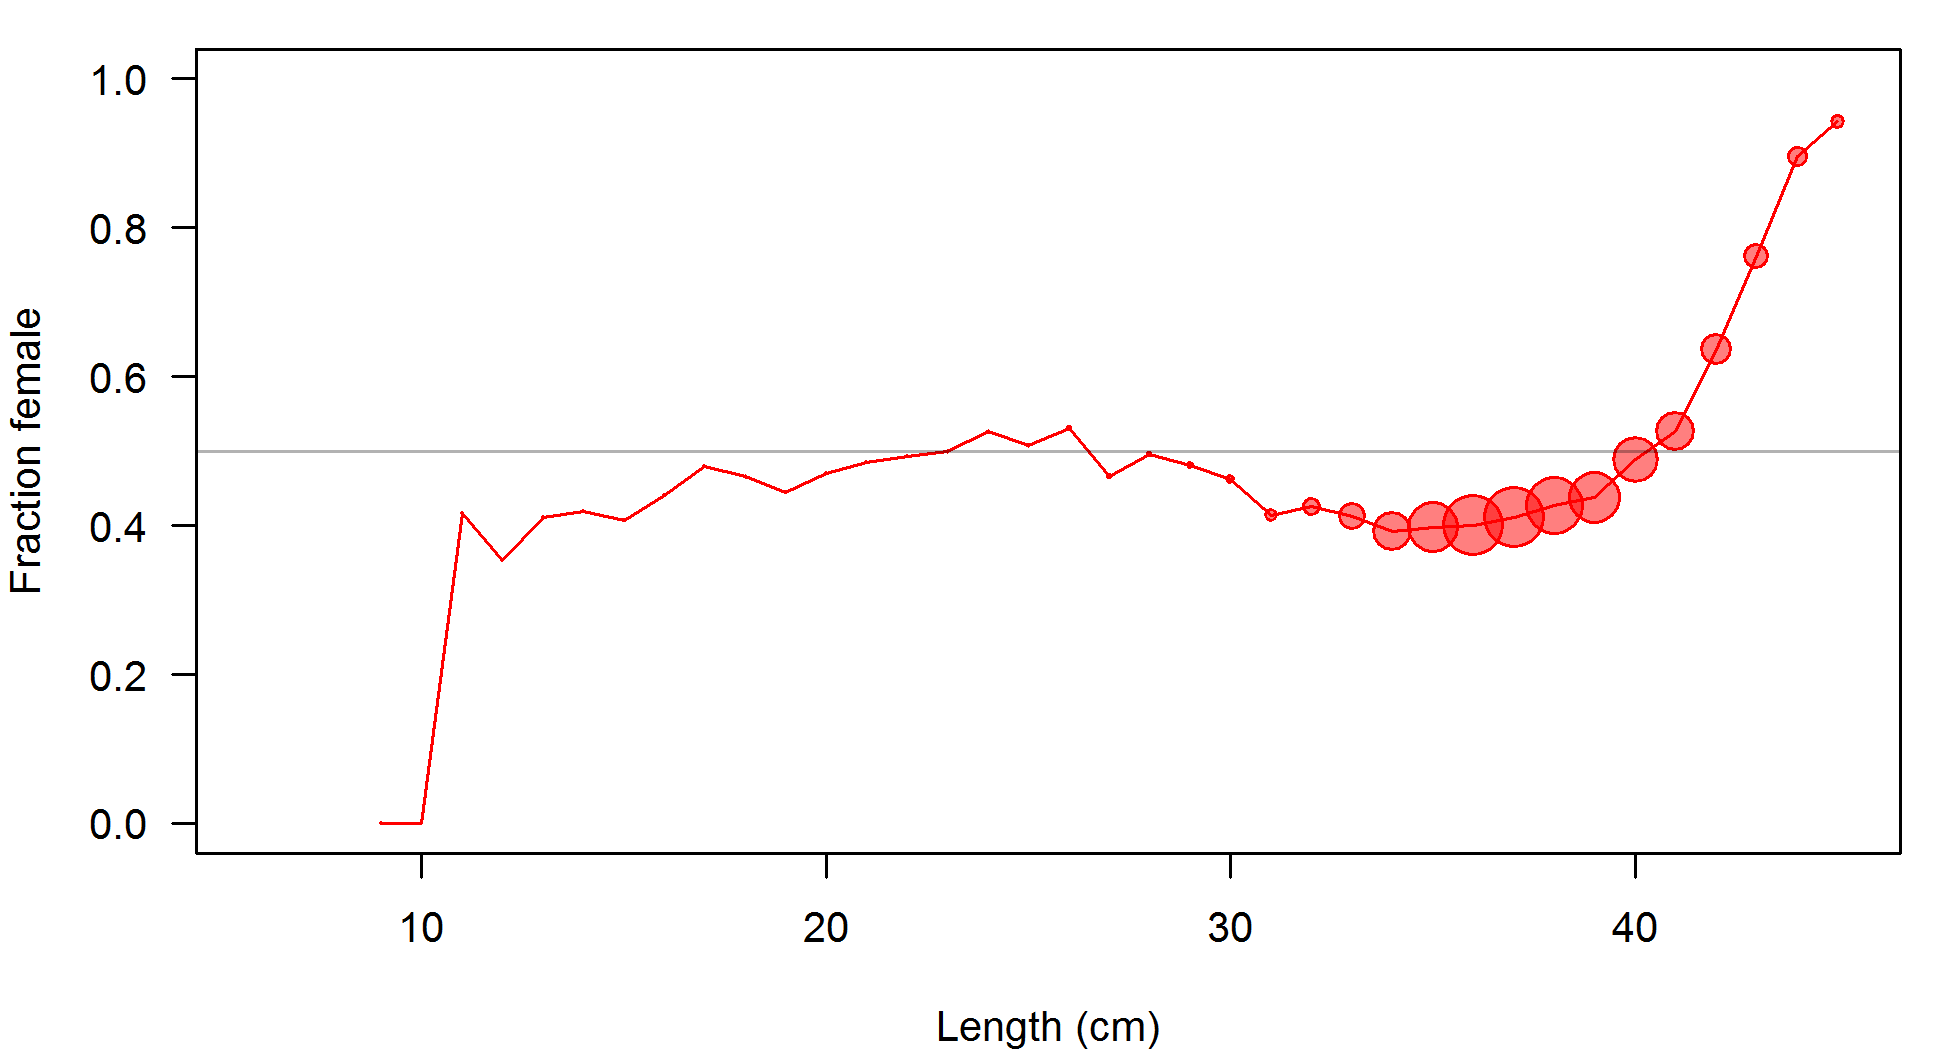
\includegraphics{Figures/allSexRatios.png}
\caption{The estimated sex ratio of Pacific ocean perch at length from
all biological data sources. \label{fig:sexratio}}
\end{figure}

\begin{figure}
\centering
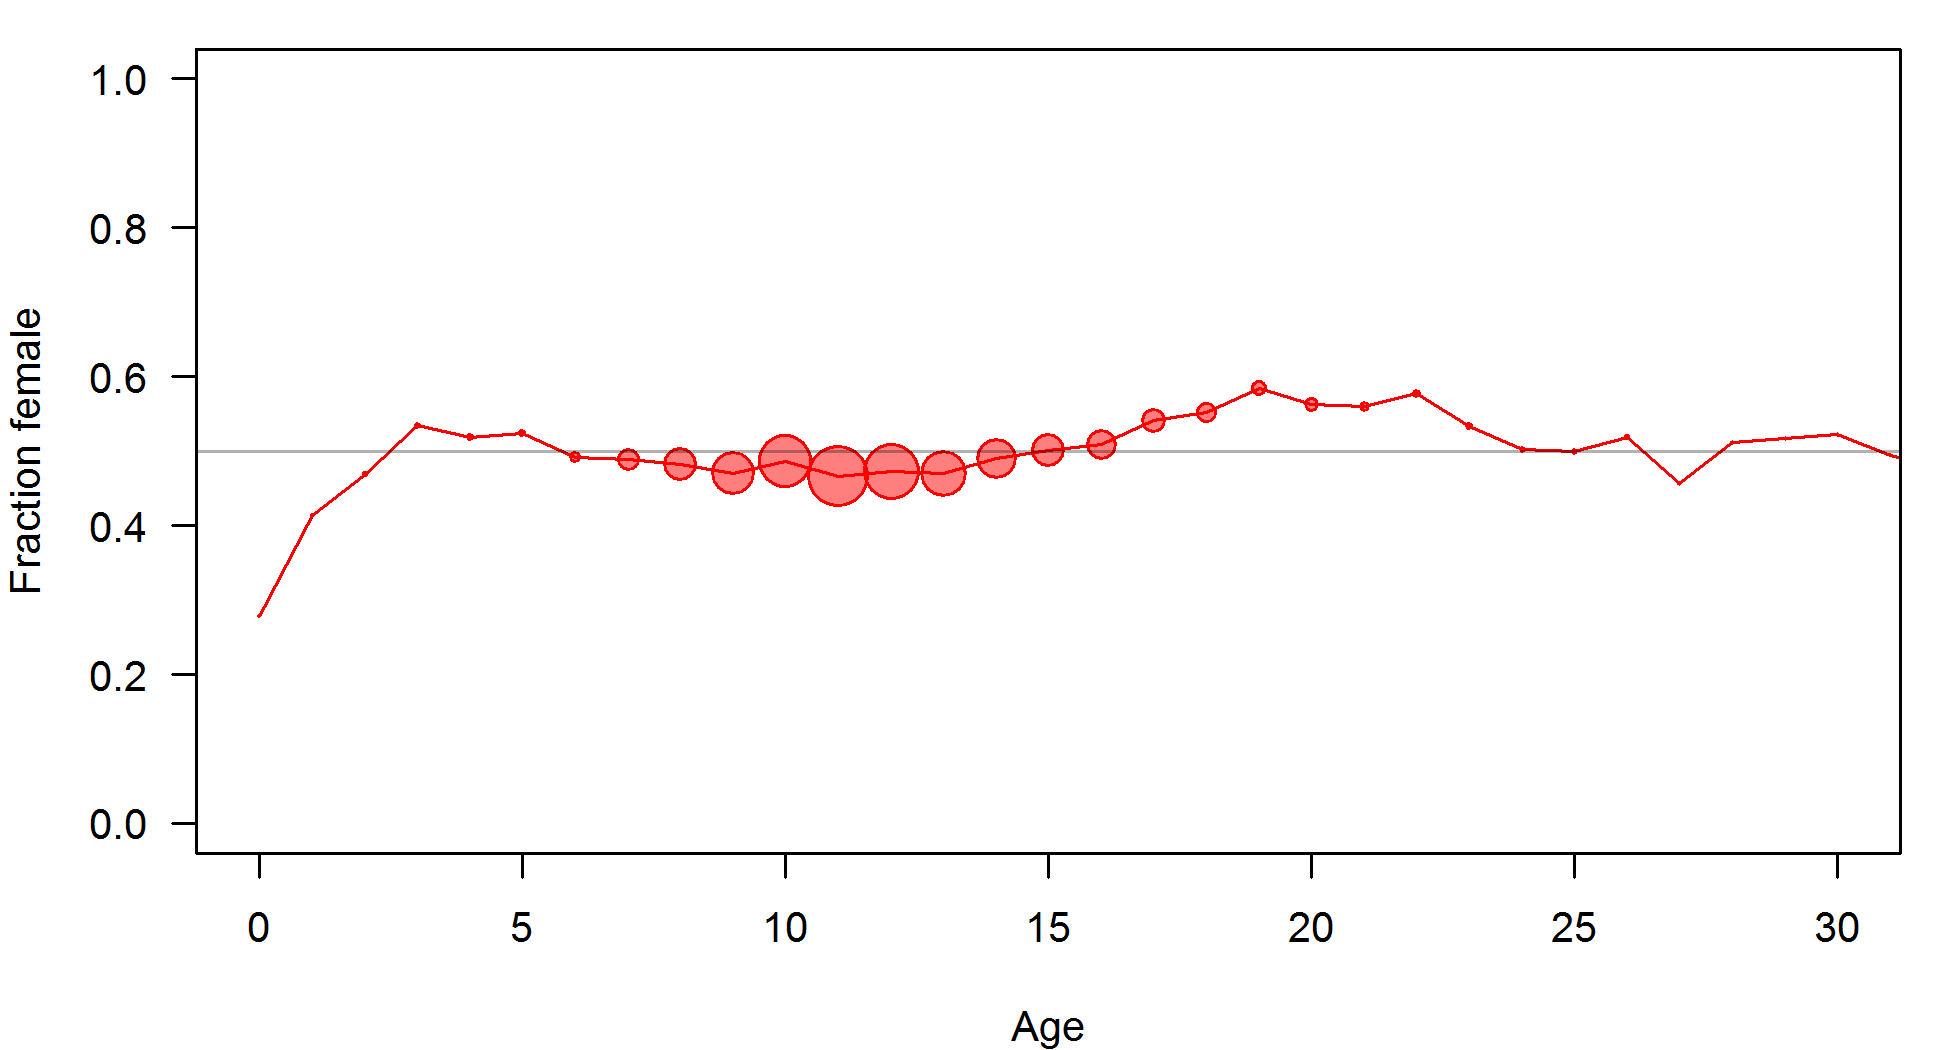
\includegraphics{Figures/allSexRatiosAge.png}
\caption{The estimated sex ratio of Pacific ocean perch at age from all
biological data sources. \label{fig:sexratio_Age}}
\end{figure}

\begin{figure}
\centering
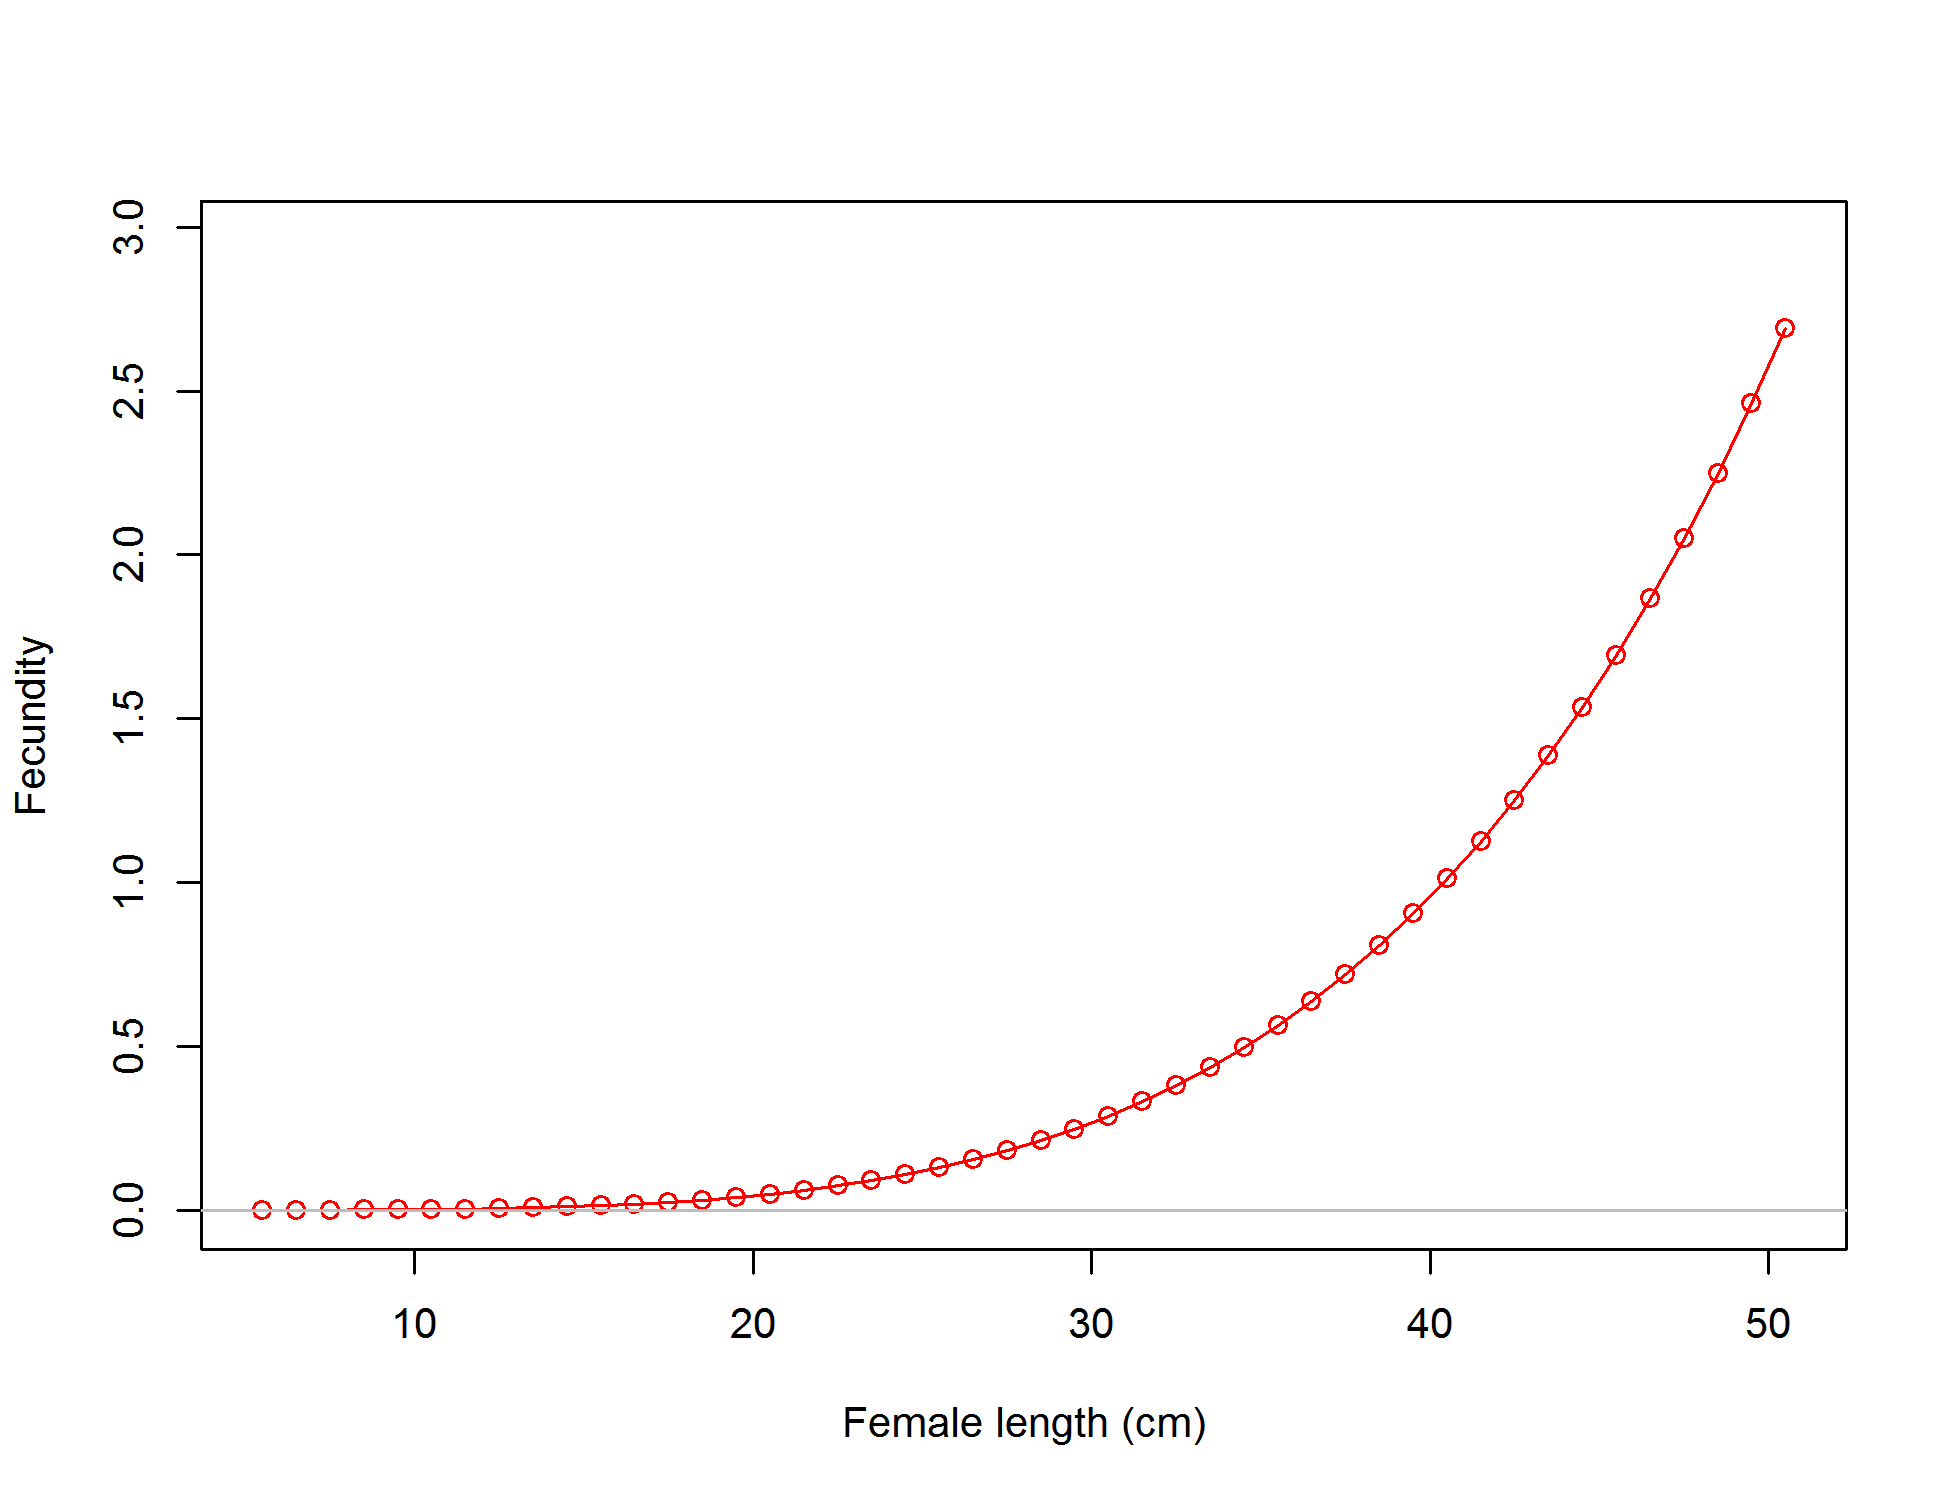
\includegraphics{r4ss/plots_mod1/bio9_fecundity_len.png}
\caption{Fecundity at length of Pacific ocean perch in the Base model.
\label{fig:fecundity}}
\end{figure}

\FloatBarrier

\FloatBarrier

\FloatBarrier

\FloatBarrier

\FloatBarrier

\FloatBarrier

\FloatBarrier
<!-- ***********MODEL 2 REFERENCE POINTS FIGURES  -- IF NEEDED ************ -->

\newpage

\color{black}

\section*{References}\label{references}
\addcontentsline{toc}{section}{References}

\renewcommand{\thepage}{}

\hypertarget{refs}{}
\hypertarget{ref-bradburn_2003_2011}{}
Bradburn, M., Keller, A., and Horness, B. 2011. The 2003 to 2008 US West
Coast bottom trawl surveys of groundfish resources off Washington,
Oregon, and California: Estimates of distribution, abundance, length,
and age composition. US Department of Commerce, National Oceanic;
Atmospheric Administration, National Marine Fisheries Service.

\hypertarget{ref-chilton_age_1982}{}
Chilton, D.E., and Beamish, R.J. 1982. Age determination methods for
fishes studied by the Groundfish Program at the Pacific Biological
Station. {[}Ottawa:{]} Minister of Supply; Services Canada.

\hypertarget{ref-dick_meta-analysis_2017}{}
Dick, E., Beyer, S., Mangel, M., and Ralston, S. 2017. A meta-analysis
of fecundity in rockfishes (genus \emph{Sebastes}). Fisheries Research
\textbf{187}: 73--85. doi:
\href{https://doi.org/10.1016/j.fishres.2016.11.009}{10.1016/j.fishres.2016.11.009}.

\hypertarget{ref-dick_modeling_2009}{}
Dick, E.J. 2009. Modeling the Reproductive Potential of Rockfishes
(\emph{Sebastes} Spp.). ProQuest. Available from
\url{http://books.google.com/books?hl=en\&lr=\&id=0d6-3rhfynkC\&oi=fnd\&pg=PR7\&dq=\%22Synthesis+of+findings+regarding+the+reproductive\%22+\%22C:+Linear+interpolation+algorithms\%22+\%22for+yellowtail+rockfish+(S.+flavidus)\%22+\%22greater+than+zero,+based+on+the+2-level+relative+fecundity\%22+\%22A:+Methods+for+data+recovery+from+published\%22+\&ots=NR0UylgymD\&sig=58IaN_a3pJeYTPYVmJ1NYMABmvE}
{[}accessed 27 February 2017{]}.

\hypertarget{ref-francis_data_2011}{}
Francis, R.C., and Hilborn, R. 2011. Data weighting in statistical
fisheries stock assessment models. Canadian Journal of Fisheries and
Aquatic Sciences \textbf{68}(6): 1124--1138. doi:
\href{https://doi.org/10.1139/f2011-025}{10.1139/f2011-025}.

\hypertarget{ref-gunderson_population_1977}{}
Gunderson, D.R. 1977. Population biology of Pacific ocean perch,
\emph{Sebastes alutus}, stocks in the WashingtonQueen Charlotte Sound
region and their response to fishing. Fishery Bulletin \textbf{75}:
369--403. Available from
\url{http://fishbull.noaa.gov/75-2/gunderson.pdf} {[}accessed 27
February 2017{]}.

\hypertarget{ref-gunderson_results_1978}{}
Gunderson, D.R. 1978. Results of cohort analysis for Pacific ocean perch
stocks off British Columbia, Washington, and Oregon and an evaluation of
alternative rebuilding strategies for these stocks. Pacific Fishery
Management Council, 7700 Ambassador Place NE, Suite 200, Portland, OR
97220.

\hypertarget{ref-gunderson_trade-off_1997}{}
Gunderson, D.R. 1997. Trade-off between reproductive effort and adult
survival in oviparous and viviparous fishes. Canadian Journal of
Fisheries and Aquatic Sciences \textbf{54}(5): 990--998. Available from
\url{http://www.nrcresearchpress.com/doi/abs/10.1139/f97-019}
{[}accessed 27 February 2017{]}.

\hypertarget{ref-gunderson_distribution_1980}{}
Gunderson, D.R., and Sample, T.M. 1980. Distribution and abundance of
rockfish off Washington, Oregon and California during 1977. Northwest;
Alaska Fisheries Center, National Marine Fisheries Service. Available
from \url{http://spo.nmfs.noaa.gov/mfr423-4/mfr423-42.pdf} {[}accessed
28 February 2017{]}.

\hypertarget{ref-gunderson_status_1977}{}
Gunderson, D.R., Westrheim, S., Demory, R., and Fraidenburg, M. 1977.
The status of Pacific ocean perch (\emph{Sebastes alutus}) stocks off
British Columbia, Washington, and Oregon in 1974.

\hypertarget{ref-hamel_method_2015}{}
Hamel, O.S. 2015. A method for calculating a meta-analytical prior for
the natural mortality rate using multiple life history correlates. ICES
Journal of Marine Science: Journal du Conseil \textbf{72}(1): 62--69.
doi:
\href{https://doi.org/10.1093/icesjms/fsu131}{10.1093/icesjms/fsu131}.

\hypertarget{ref-hannah_age-modulated_2007}{}
Hannah, R., and Parker, S. 2007. Age-modulated variation in reproductive
development of female Pacific Ocean perch (\emph{Sebastes alutus}) in
waters off Oregon. Alaska Sea Grant, University of Alaska Fairbanks. pp.
1--20. doi:
\href{https://doi.org/10.4027/bamnpr.2007.01}{10.4027/bamnpr.2007.01}.

\hypertarget{ref-hoenig_empirical_1983}{}
Hoenig, J.M. 1983. Empirical use of longevity data to estimate mortality
rates. Fishery Bulletin \textbf{82}: 898--903. Available from
\url{http://fishbull.noaa.gov/81-4/hoenig.pdf} {[}accessed 28 February
2017{]}.

\hypertarget{ref-karnowski_historical_2014}{}
Karnowski, M., Gertseva, V., and Stephens, A. 2014. Historical
Reconstruction of Oregon's Commercial Fisheries Landings. Oregon
Department of Fish; Wildlife, Salem, OR.

\hypertarget{ref-mcallister_bayesian_1997}{}
McAllister, M.K., and Ianelli, J.N. 1997. Bayesian stock assessment
using catch-age data and the sampling - importance resampling algorithm.
Canadian Journal of Fisheries and Aquatic Sciences \textbf{54}:
284--300. Available from
\url{http://www.nrcresearchpress.com/doi/pdf/10.1139/f96-285}
{[}accessed 10 March 2017{]}.

\hypertarget{ref-mccoy_predicting_2008}{}
McCoy, M.W., and Gillooly, J.F. 2008. Predicting natural mortality rates
of plants and animals. Ecology Letters \textbf{11}(7): 710--716. doi:
\href{https://doi.org/10.1111/j.1461-0248.2008.01190.x}{10.1111/j.1461-0248.2008.01190.x}.

\hypertarget{ref-methot_stock_2013}{}
Methot, R.D., and Wetzel, C.R. 2013. Stock synthesis: A biological and
statistical framework for fish stock assessment and fishery management.
Fisheries Research \textbf{142}: 86--99. doi:
\href{https://doi.org/10.1016/j.fishres.2012.10.012}{10.1016/j.fishres.2012.10.012}.

\hypertarget{ref-pikitch_evaluation_1988}{}
Pikitch, E.K., Erickson, D.L., and Wallace, J.R. 1988. An evaluation of
the effectiveness of trip limits as a management tool. Northwest; Alaska
Fisheries Center, National Marine Fisheries Service NWAFC Processed
Report. Available from
\url{https://www.afsc.noaa.gov/Publications/ProcRpt/PR1988-27.pdf}
{[}accessed 28 February 2017{]}.

\hypertarget{ref-ralston_documentation_2010}{}
Ralston, S., Pearson, D.E., Field, J.C., and Key, M. 2010. Documentation
of the California catch reconstruction project. US Department of
Commerce, National Oceanic; Atmospheric Adminstration, National Marine.

\hypertarget{ref-rogers_species_2003}{}
Rogers, J. 2003. Species allocation of \emph{Sebastes} and
\emph{Sebastolobus} species caught by foreign countries off Washington,
Oregon, and California, U.S.A. in 1965-1976. Unpublished document.

\hypertarget{ref-rogers_numerical_1992}{}
Rogers, J.B., and Pikitch, E.K. 1992. Numerical definition of groundfish
assemblages caught off the coasts of Oregon and Washington using
commercial fishing strategies. Canadian Journal of Fisheries and Aquatic
Sciences \textbf{49}(12): 2648--2656. Available from
\url{http://www.nrcresearchpress.com/doi/abs/10.1139/f92-293}
{[}accessed 9 March 2017{]}.

\hypertarget{ref-seeb_genetic_1988}{}
Seeb, L.W., and Gunderson, D.R. 1988. Genetic variation and population
structure of Pacific ocean perch (\emph{Sebastes alutus}). Canadian
Journal of Fisheries and Aquatic Sciences \textbf{45}(1): 78--88.
Available from
\url{http://www.nrcresearchpress.com/doi/abs/10.1139/f88-010}
{[}accessed 28 February 2017{]}.

\hypertarget{ref-then_evaluating_2015}{}
Then, A.Y., Hoenig, J.M., Hall, N.G., and Hewitt, D.A. 2015. Evaluating
the predictive performance of empirical estimators of natural mortality
rate using information on over 200 fish species. ICES Journal of Marine
Science \textbf{72}(1): 82--92. doi:
\href{https://doi.org/10.1093/icesjms/fsu136}{10.1093/icesjms/fsu136}.

\hypertarget{ref-thorson_comparing_2017}{}
Thorson, J.T., and Barnett, L.A.K. 2017. Comparing estimates of
abundance trends and distribution shifts using single- and multispecies
models of fishes and biogenic habitat. ICES Journal of Marine Science:
Journal du Conseil: fsw193. doi:
\href{https://doi.org/10.1093/icesjms/fsw193}{10.1093/icesjms/fsw193}.

\hypertarget{ref-weinberg_estimation_2002}{}
Weinberg, J.R., Rago, P.J., Wakefield, W.W., and Keith, C. 2002.
Estimation of tow distance and spatial heterogeneity using data from
inclinometer sensors: An example using a clam survey dredge. Fisheries
Research \textbf{55}(1--3): 49--61. doi:
\href{https://doi.org/10.1016/S0165-7836(01)00292-2}{10.1016/S0165-7836(01)00292-2}.

\hypertarget{ref-wilkins_condition_1983}{}
Wilkins, M., and Golden, J. 1983. Condition of the Pacific ocean perch
resource off Washington and Oregon during 1979: Results of a cooperative
trawl survey. North American Journal of Fisheries Management \textbf{3}:
103--122.

\hypertarget{ref-withler_co-existing_2001}{}
Withler, R., Beacham, T., Schulze, A., Richards, L., and Miller, K.
2001. Co-existing populations of Pacific ocean perch, Sebastes alutus ,
in Queen Charlotte Sound, British Columbia. Marine Biology
\textbf{139}(1): 1--12. doi:
\href{https://doi.org/10.1007/s002270100560}{10.1007/s002270100560}.

\hypertarget{ref-zimmermann_influence_2003}{}
Zimmermann, M., Wilkins, M., Weinberg, K., Lauth, R., and Shaw, F. 2003.
Influence of improved performance monitoring on the consistency of a
bottom trawl survey. ICES Journal of Marine Science \textbf{60}(4):
818--826. doi:
\href{https://doi.org/10.1016/S1054-3139(03)00043-2}{10.1016/S1054-3139(03)00043-2}.

\end{document}
